\documentclass[12pt]{book}
%%%%%%%%%% Packages language %%%%%%%%%%
\usepackage[utf8]{inputenc}
\usepackage{listings}   % inline code
\usepackage{natbib}     % bib
\usepackage{verbatim}   % comments
\usepackage{url}        % cite url
\usepackage{epigraph}   % fucks sake
%%%%%%%%%%%%% MATHS %%%%%%%%%%%%%%%%%%%%
\usepackage{amsmath} 
\usepackage{mathtools}
\usepackage{physics}    % oh yeah
\usepackage{amssymb} 
\usepackage{qcircuit}   % awesome circuits
\usepackage{gensymb}    % for \degree symbol
%%%%%%%%% Figures %%%%%%%%%%%%%%%%%%%%%%%
\usepackage{graphicx} 
\usepackage{caption}    % subfigures
\usepackage{scrextend} 
\usepackage{subcaption} % sub figs again
\usepackage{float}      % images
\usepackage{hyperref}   % colourful refs
\usepackage{color}      %???
\usepackage{geometry}   % margins and spacing
\usepackage{multicol}   % Andres 
\usepackage[skins]{tcolorbox} % Andres
%%%%%%%%%%%% Table stuff %%%%%%%%%%%%%%%
\usepackage{fourier}    %? ??
\usepackage{array}      % ????
\usepackage{makecell} 
\usepackage[noblocks,affil-it]{authblk} % Andres
\usepackage{afterpage}
\usepackage{pdflscape}
\usepackage{rotating}
%%%%%%%%%% colours %%%%%%%%%%%%%%%
\definecolor{codegreen}{rgb}{0,0.6,0}
\definecolor{codegray}{rgb}{0.5,0.5,0.5}
\definecolor{codepurple}{rgb}{0.58,0,0.82}
\definecolor{backcolour}{rgb}{0.95,0.95,0.92}
\definecolor{mygray}{gray}{0.95}

%%%%%%%%%% inline code %%%%%%%%%%%%%
% For inline assembly
\lstdefinelanguage{asm}
{
    morekeywords={BRA,CLR,BTG,BSET,BCLR,BTSC,QBTX,QBTY,CNOT,MOV},
    morecomment=[l]{;},
    % space is \ space
    morestring=[s]{##}{\ },
    morestring=[s][\color{orange}]{Q}{\ },
    morestring=[s][\color{orange}]{CNO}{\ }             
}

%%%%%%%%%%%%%%%%%%%%%%%
% for C#

\lstdefinelanguage{Csharp}
{
    morekeywords={using,namespace,class,static,public,private,void,string,int,double,try,catch,return,var,new,for,foreach,while,continue,if,else,in},
    morecomment=[l]{//}, % l is for line comment
    morecomment=[s]{/*}{*/}, % s is for start and end delimiter
    morestring=[b]" 
}

%%%%%%%%%%%%%%%%%%%%%%%
% for Q#

\lstdefinelanguage{Qsharp}
{
    morekeywords={namespace,open,operation,body,Qubit,Pauli,Range,Int,Double,String,Result,Bool,let,set,mutable,true,false,One,Zero,PaulI,PauliX,PauliY,PauliZ,H,X,M,Y,Z,I,if,for,in,Controlled,Adjoint,return,adjoint,auto,controlled},
    morecomment=[l]{//}, % l is for line comment
    morestring=[b]" 
}

%%%%%%%%%%%%%%%%%%%%%%%%
\lstdefinestyle{mystyle}
{
backgroundcolor=\color{mygray},   
 commentstyle=\color{codegreen},
 keywordstyle=\color{blue},
 numberstyle=\tiny\color{codegray},
 stringstyle=\color{codepurple},
 basicstyle=\footnotesize,
 breakatwhitespace=false,         
 breaklines=true,                 
 captionpos=b,                    
 keepspaces=true,                 
 numbers=left,                    
 numbersep=5pt,                  
 showspaces=false,                
 showstringspaces=false,
 showtabs=false,                  
 tabsize=2,
 xleftmargin=2em, % this line added by Andres
 framexleftmargin=1.5em % This line added by Andres
 } 
%%%%%%%%%%%%%%%%%%%%%%
\lstset{style=mystyle}

%% use this 
%\lstinputlisting[language=Python, firstline=37, lastline=45]{code/source_filename.py}
%\lstinputlisting[language=Python, linerange={1-5,6-9}]{code/source_filename.py}


%%%%%%%%%%%%%%%%%%%%%%%%%%%%%%%%%%%%%
%Make the footnote rule extend over the full length of the footnote
\renewcommand{\footnoterule}{%
  \kern -3pt
  \hrule width \textwidth height 1pt
  \kern 2pt}

%%%%%%%%%%%%% hyperlink %%%%%%%%%%%%%%
\hypersetup{colorlinks=true,
            %citecolor=green, % changed by Andres
            citecolor=purple,
            linkcolor=blue,}
\renewcommand{\equationautorefname}{Eq.}
\renewcommand{\figureautorefname}{Fig.}
\renewcommand{\chapterautorefname}{Chapter} %C not c

%%%%%%%%%%%%% File paths %%%%%%%%%%%%%%
\graphicspath{{figures/}}
\newgeometry{left=0.8in,right=0.8in,top=1in,bottom=1in} 
%\renewcommand{\familydefault}{\ttdefault}


%%%%%%%%%%%%%%%%
\begin{document}

% Are we gonna add UoB and CDT logos?

% Please add here your title proposal
\title{\bf Quantum Meta-Programming for Dummies with a weak focus on Poisson Bullets, in the style of a book. \\ {\large The Grandest of Cohort Grand Challenges}}

% A concise quantum programming guide for the quantum software enthusiast

%%%%%%%%%%%%%%%%%%%%%%
\author[ ]{Jake Biele}
\author[ ]{Andrés Ducuara}
\author[ ]{Jonathan Frazer}
\author[ ]{Huili Hou}
\author[ ]{Friederike Jöhlinger}
\author[ ]{Ankur Khurana}
\author[ ]{Lana Mineh}
\author[ ]{David Payne}
\author[ ]{Ben Sayers}
\author[ ]{John Scott}
\author[ ]{Dominic Sulway}
\author[ ]{last but not least, Oliver Thomas}

\affil[ ]{ {\small Quantum Engineering Centre for Doctoral Training \protect \\ H. H. Wills Physics Laboratory and Department of Electrical \& Electronic Engineering, University of Bristol, BS8 1FD, UK}}
%%%%%%%%%%%%%%%%%%%%%%%%%%%%%%%
%%%%%%%%%%%%%%
\begin{comment} % commented out by ______
\author[ ]{J. Biele}
\author[ ]{A. Ducuara}
\author[ ]{J. Frasure}
\author[ ]{H. Hou}
\author[ ]{F. Jöhlinger}
\author[ ]{A. Khurana}
\author[ ]{L. Mineh}
\author[ ]{D. Payne}
\author[ ]{B. Sayers}
\author[ ]{J. Scott}
\author[ ]{D. Sulway}
\author[ ]{O. Thomas}

\affil[ ]{ {\small Quantum Engineering Technology Labs, H. H. Wills Physics Laboratory and \\ Department of Electrical \& Electronic Engineering, University of Bristol, BS8 1FD, UK}}
\end{comment}
%%%%%%%%%%%%%
%%%%%%%%%%%%%
\date{\today}
\maketitle

%%%%%%%%%%%%%%%%%%%%%%%%%%%%%%%
\chapter*{Preface}
\addcontentsline{toc}{chapter}{Preface}

% Won't someone write me?

Quantum programming, as you might expect, requires understanding of both quantum theory and programming. we have designed this guide to cover from the basics of quantum theory and programming, to the implementation of quantum programs in already existing quantum computers. Whether you are an experienced programmer with little or no experience with quantum, a quantum theoretician with little or no experience with programming, or an enthusiast willing to get into the field of quantum computing, we believe that you might find something useful out of this guide.\\ 
% This guide will help filling knowledge gaps in the emergent field of quantum software engineering. 
%  (and quantum video games!)

\noindent
We are living in the so-called second quantum revolution and quantum computing is leading the way. The construction of quantum computers in the last few years has led to an explosion in the development of quantum software, and so is the need for quantum programming guides. In this guide we provide a self contained introduction to both quantum theory and programming, an overview of current quantum programming languages/libraries, example programs and exercises implemented in different quantum languages/libraries, so that you acquire the fundamentals to start writing your own quantum programs.\\
% \footnote{With solutions at the end of the guide Yayy!}

\noindent
We are the fourth cohort of the Quantum Engineering Centre for Doctoral Training (QE-CDT) at the University of Bristol, and this guide is the outcome of our quantum grand challenge on quantum programming. We are addressing the subject in the way that we would have liked to learn about it, with tips and tricks that we have found along this journey, that the future quantum software engineers might find useful.\\

\noindent
Quantum regards!\\

\noindent
QE-CDT Cohort 4\\

\noindent
September, 2018

% please dont delete yet xd
\begin{comment}

%%%%%%%%%%%%%%%%%%%%%%%%%%%%%%%
\subsection{Some Quotes that we can use throughout the guide}

This one from \cite{WZ2017}

\emph{Third, scientists need to establish a quantum programming community to nurture an ecosystem of software. This community must be interdisciplinary, inclusive and focused on applications.}\\

This one from \cite{QSmanifesto}

\emph{One of the challenges the quantum computing field currently faces is a shortage of people that have been trained to write and develop quantum software.}\\

This one from \cite{QSmanifesto}

\emph{Just as classical computers are meaningless pieces of hardware without appropriate software, quantum computers need quantum software to function.}\\


“So do not take the lecture too seriously, feeling that you really have to understand in terms of some model what I am going to describe, but just relax and enjoy it.” (Feynman [Fey65])\\


From \cite{Preskill2012}\\

Attaining quantum supremacy and exploring its consequences will be among the great challenges facing 21st century science, and our imaginations are poorly equipped to envision the scientific rewards of manipulating highly entangled quantum states, or the potential benefits of advanced quantum technologies. As we rise to the call of the entanglement frontier, we should expect the unexpected.\\

\cite{Preskill2018} \\

The history of classical computing teaches us that when hardware becomes available that stimulates and accelerates the development of new algorithms.\\

The truly transformative quantum technologies of the future are probably going to have to be fault tolerant, and because of the very hefty overhead cost of quantum error correction, the era of fault-tolerant quantum computing may still be rather distant.\\

All quantumists should appreciate that our field can fulfill its potential only through sustained, inspired effort over decades. If we pay that price, the ultimate rewards will more than vindicate our efforts.\\

\end{comment}

\section{Things to be careful with and TODO list}

\begin{itemize}
\item Python 3!
\item Check same spelling of pyQuil, Project Q, Qiskit and Q\#
\item Check Use of Active voice
\item Please use autoref instead of ref alone
\item no adjoints!
\item reversible NOT unitary 
\item move all sections to be consisten sizes. NO SECTION*{} only subsection
\end{itemize}

%%%%%%%%%%%%%%%%%%%%%%%%%%%%%%%
%\newpage

%%%%%%%%%%%%%%%%%%%%%%%%%%%%%%%%
%%%%%%%%%%%%%%%%%%%%%%%%%%%%%%%%
\chapter*{How to use this guide (loading...)}
%%%%%%%%%%%%%%%%%%%%%%%%%%%%%%%%
%%%%%%%%%%%%%%%%%%%%%%%%%%%%%%%%

Depending on your background, you might want to approach our guide differently. Here we describe three recommended paths depending on your background, but feel free to explore our guide as you wish!

%%%%%%%%%%%%%%%%%%%%%%%%%%%%%%%%%%%%%%%%%
\subsection*{Profile 1: The programmer}

You can start from Chapter 1, if things are getting difficult you might want to refresh your mind on linear algebra and vector spaces in \autoref{Advancedtopics}, and then come back to \autoref{Background}. From here you can easily follow chapter two which uses mostly Python.

%%%%%%%%%%%%%%%%%%%%%%%%%%%%%%%%%%%%%
\subsection*{Profile 2: The quantum theoretician}

Depending on you programming experience, you might want to check our mini tutorial in python \autoref{pythontutorial}. Then you can address \autoref{QPL}, simple programs implemented in different languages.

%%%%%%%%%%%%%%%%%%%%%%%%%%%%%%%%%%%%%%%%%
\subsection*{Profile 3: The Enthusiast}

We recommend first a fast course on quantum mechanics. \autoref{Advancedtopics} then \autoref{Background}. Then our basics for programming, \autoref{pythontutorial}. After this, you can comfortably go to \autoref{QPL}.

\vspace{1cm}

\noindent
If you wanna explore more on Q theory references. Describing these references \cite{nielsen_chuang_2010}, \cite{Preskill}, \cite{Watrous}

\noindent
If you wanna explore more on programming references. Python coursera \cite{PythonCoursera} what else here?

%%%%%%%%%%%%%%%%
\tableofcontents

%%%%% change linespacing between paragraphs
\setlength{\parskip}{0.5em}

%%%%%%%%%%%%%%%%%%%%%%%%%%%%%%%%%%
\chapter*{Introduction}
\addcontentsline{toc}{chapter}{Introduction}

%\epigraph{[Quantum computation] does not merely make computer science
%a branch of physics. \\ It also makes part of experimental physics into a %branch of computer science.}{\\ David Deutsch \\ Quantum theory, the %Church-Turing principle, and the universal quantum computer}

Quantum mechanics is one of the most well-tested theories in existence. It is also one of the most unintuitive, revealing aspects of nature at nanoscopic scales which are entirely incompatible of our a human's experience of the world. \\

There are two main facets which differentiate quantum from classical theory. The first, from which the field derives its name, is the quantisation of properties of a particle such as charge, angular momentum, and energy. This feature has already changed the world substantially over the course of the last 70 years. In addition to technologies such as the laser and magnetic resonant imaging (MRI) \cite{ioplasers, odaibo2012quantumMRI}, perhaps the greatest impact has been made through the manipulation of semiconductors. Since the invention of the first transistor in 1947 \cite{Bardeen1948}, semiconductor technology has laid the groundwork for scalable computing, bringing us into the the current information age. \\

The development of this technology comes at a critical time in the conventional silicon industry. The famous `Moore's law', hypothesised in its current form in 1975, stated that the number of transistors per square inch would double every two years. This rule of thumb models the exponential scaling which computing power has followed since its conception incredibly well, as seen in \autoref{fig:Moore's_Law}. This was driven predominantly by the cost and power consumption per transistor going down as feature sizes decreased \cite{MooresLawEconomist}.  However, now increasingly small feature sizes have resulted in energy efficiencies and profitability are starting to plateau, while technical issues continue to increase. Some of these issues are in part due to quantum effects such as `tunnelling', where an electron is able to access regions in space where, classically, it would be have insufficient energy to reach.   \\

\begin{figure}[!ht]
	\centering
	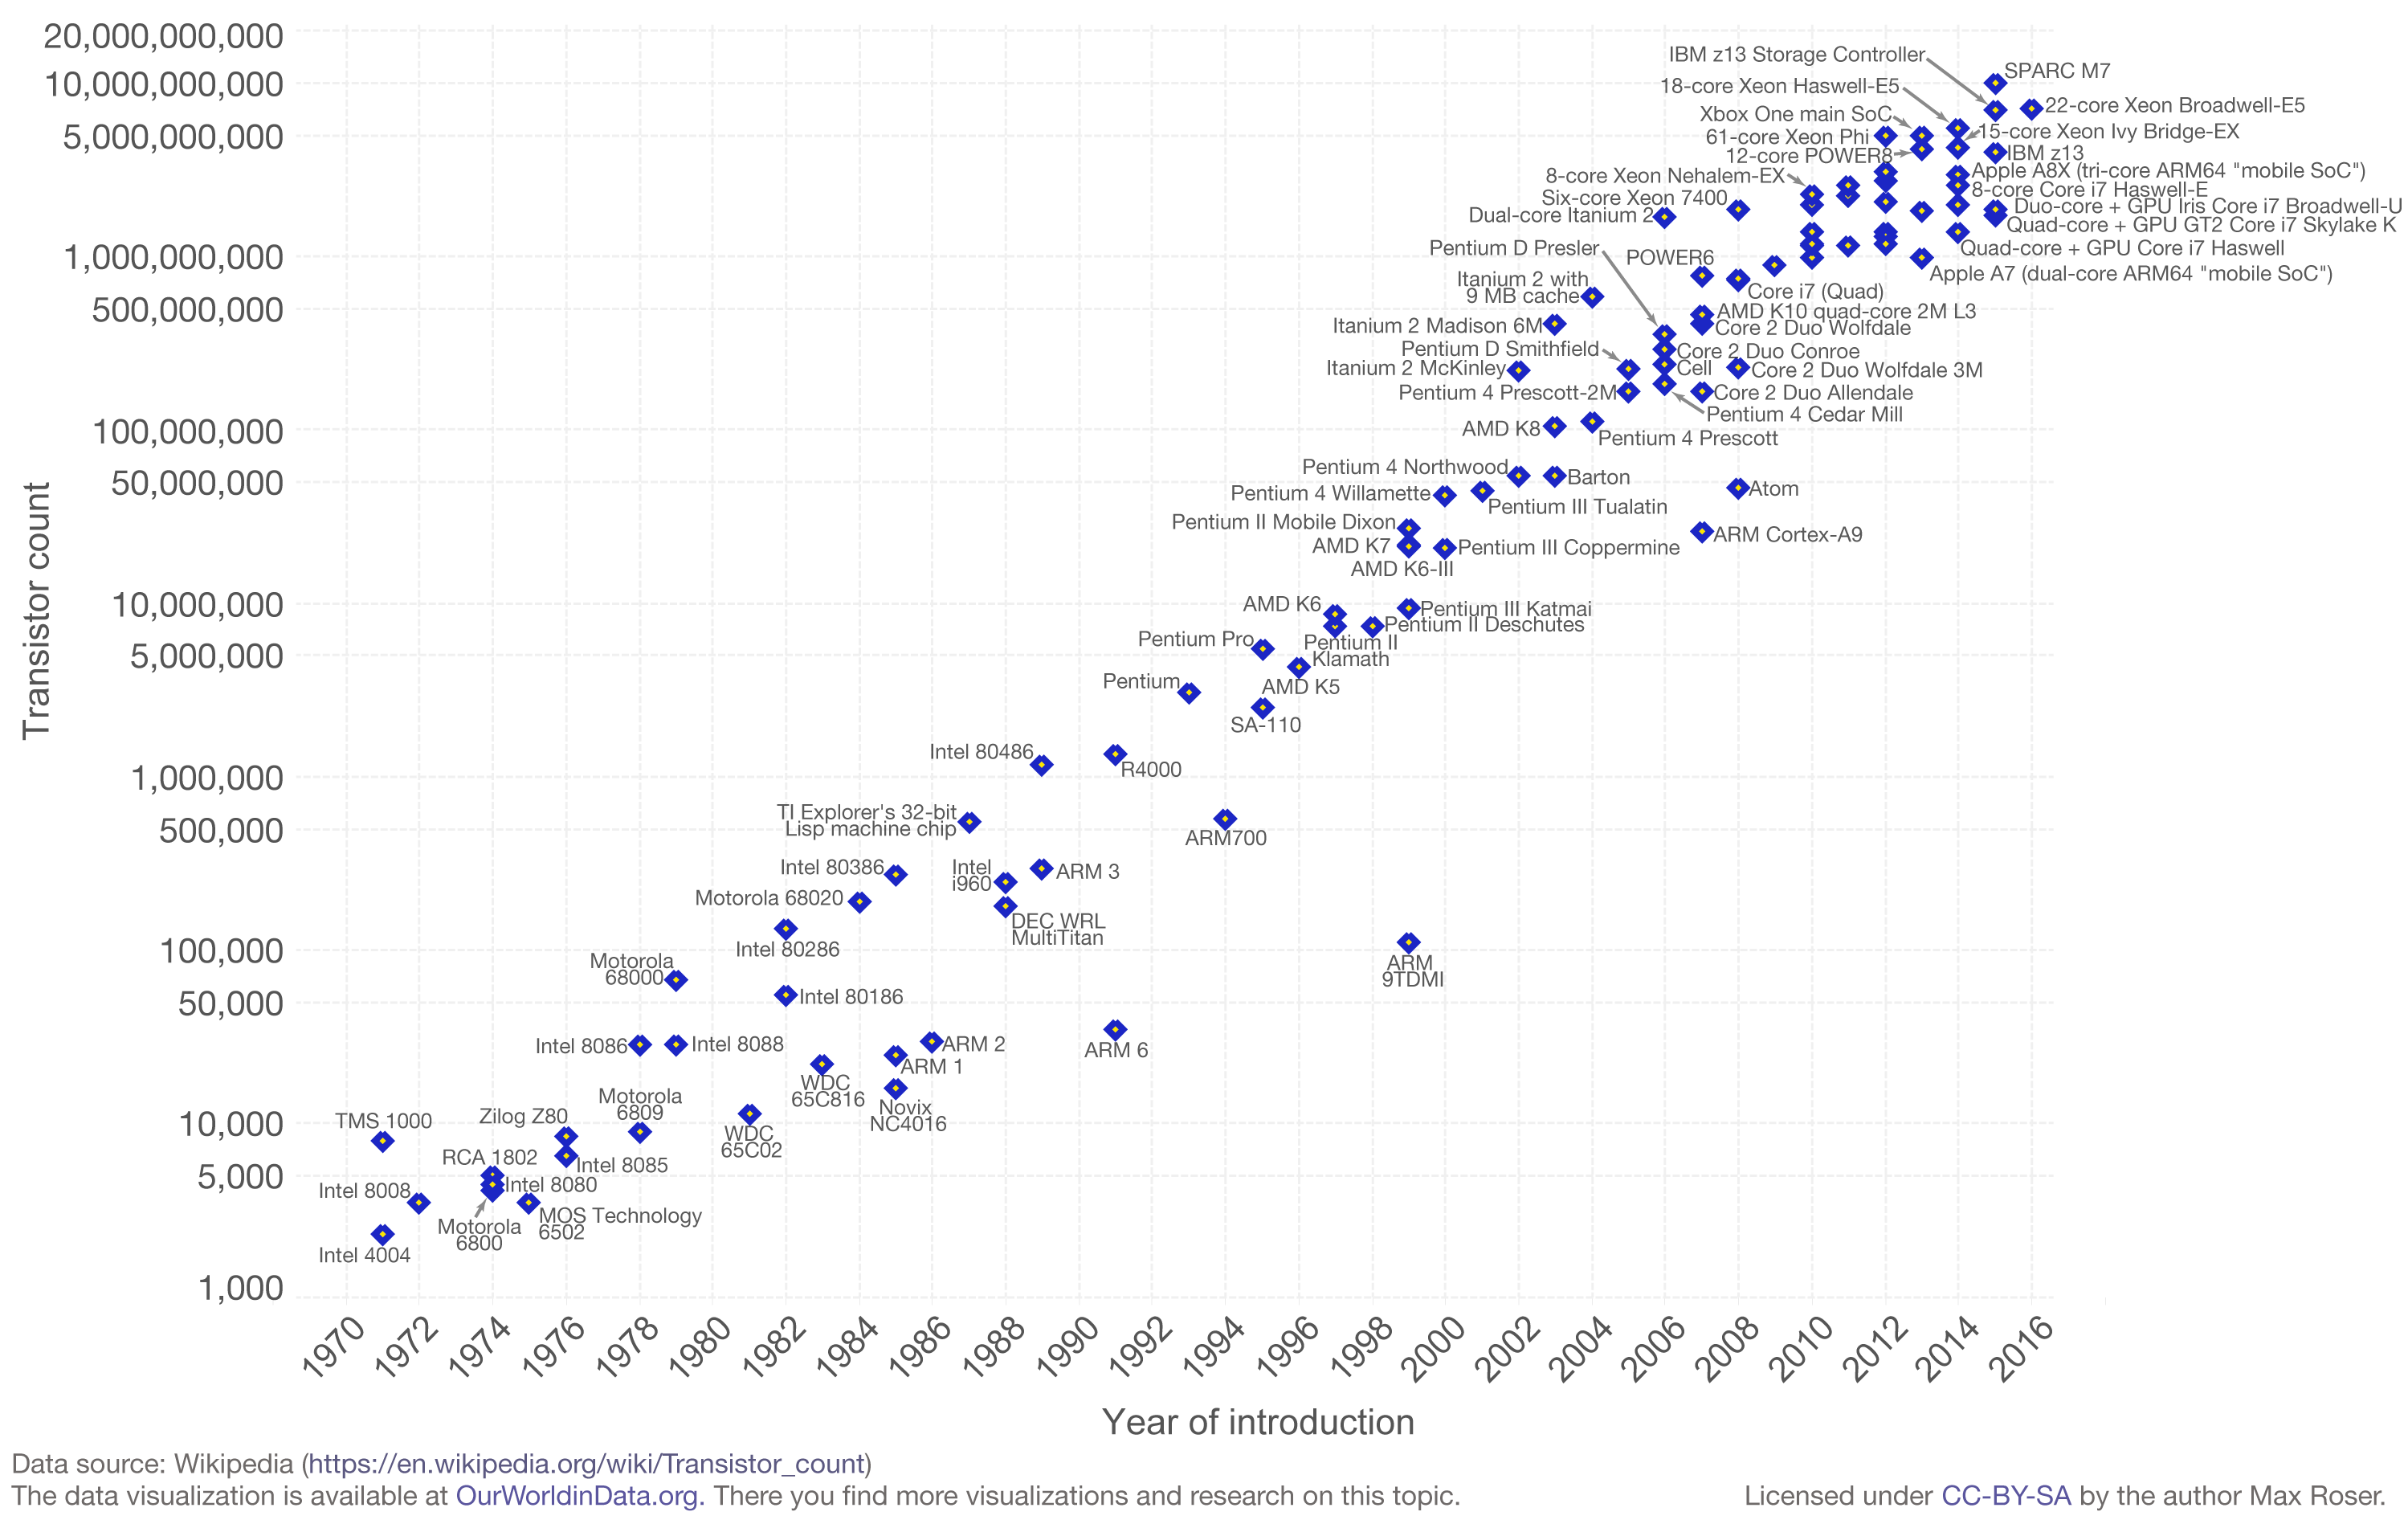
\includegraphics[width = \linewidth]{Moores_Law.png}
	\caption{Chart showing Moore's law, with a logarithmic increase in transistor 	count on each chip from 1970-2016.}
	\label{fig:Moore's_Law}
\end{figure}

In fact, this feature is already used in so-called quantum annealers such as those built by D-Wave \cite{D-Wave}. These machines use tunneling to find optimal solutions to a range of optimisation problems, where  This example of tunnelling is related to the so-called `wave-particle duality' which is the second key feature of quantum mechanics. The distinction between waves and particles, whose behaviour is well established in classical physics, becomes blurred. Every object in the universe, depending on their energy and confinement, will display both of these aspects to some degree. \\

The tantalising promise of quantum computing is hidden in this property. Particles such as electrons, which have comprised the backbone of electricity and classical information for the past century, have the ability to behave in a wave-like manner: they could contain not just the binary bit choices of 0 or 1,  but one of an infinite number of continuous values, called `qubits'. The ability to investigate the effect of a process on both 0 and 1 bits simultaneously means that quantum computers have the ability to scale exponentially (instead of polynomially) with the resources  that are put in. This scaling is crucial. Currently for computationally difficult tasks (problems in science, AI and more) supercomputers must be used, which take up massive amounts of space and are costly to build and run. The current state of the art is shown in  \autoref{fig:Summit}. If instead our computational scaling was exponential instead of polynomial we could perform the same task with many fewer qubits than bits - as the problem becomes more exaggerated \footnote{A classic example of the power of exponential scaling is given by the legend of a vizier who presented a gift to his King. The king asked what he wanted in return, and the vizier replied that he wanted rice. Precisely, he wanted one grain of rice on the first square of the chessboard, two grains of rice on the second, four grains on the third, and so on, doubling on each square. This bankrupts the king, who has to find $2^{63}$ grains of rice for the last square alone. This is $\sim 100$ times greater than the \emph{current} global annual food production. (At $\sim 10^{12}$kg \cite{Globalfoodproduction})}. Combined with entanglement to allow our qubits to influence each other in these states, we can harness a form of parallelism that results from the wave-like nature of controlled particles.  \\

While in general it is doubtful that a quantum computer will be universally  `faster' than a classical computer, and is much harder to engineer, there is significant potential to outperform conventional computers at certain tasks. While the amount of information processing in a conventional computer scales linearly with the number of bits, a quantum computer scales exponentially with the number of qubits for these tasks. Thus adding a single extra qubit could double the computing power. These are discussed, along with the quantum algorithms used to implement them, in \autoref{Algorithmsandapplications}. At the point when quantum computers are able to outperform classical supercomputers at a task, the so-called `quantum supremacy' \cite{Preskill2012} will have been achieved. \\

% are we mentioning that we can simulate around 50-qubit Q computer with classical computers?

% Further references on Q supremacy. First time defined \cite{Preskill2012}, recently proposed algorithm \cite{QKitchenSinks2018}, theoretical work on the amount of qubits needed for it \cite{Harrow2018}, the article suggesting supremacy with Boson sampling is far away \cite{BSsupremacy2017}.

These tasks range from aiding the fields of medicine, chemistry and materials with applications including creating more powerful simulations\footnote{This application - the simulation of large, complex many body systems - was in fact one of the very first motivators for the development of quantum computers, most famously by Richard Feynman \cite{Feynman1982simulating}.}\cite{Georgescu2014Sim}; providing potential speedups for AI and machine learning \cite{Biamonte2017QML}; assisting with modelling complex logistics problems; and improving financial models \cite{Schaden2002quantumfinance}.\\

However, achieving this potential does not come without significant engineering difficulties. Readout or detection of the information in the qubit destroys the information contained within, resulting in us reverting to the classical bit values with an some probabilities. These probabilities  are a fundamental (and irremovable) part of quantum theory, providing the link between \ldots Furthermore, the technology is still very young and undeveloped. Algorithms exist for many of the applications above, but there may be many more as yet undiscovered. Academic institutions, large corporations (including Google \cite{googleqai, bristlecone}, IBM, \cite{ibmqweb} and Intel \cite{intelqcomp}) and small start-ups, sucha as Rigetti, \cite{rigettihome}, alike have invested heavily in hardware. There are a wide range of platforms and architectures, including but not limited to superconducting qubits \cite{bristlecone}, ion traps \cite{steane1997ionTrap}, quantum dots \cite{loss1998quantumdots}, spin qubits in silicon \cite{intelSCspinqubits}, and silicon poisson bullets \cite{RudolphSiliconPhotonicsQC}. \\

\begin{figure}
    \centering
    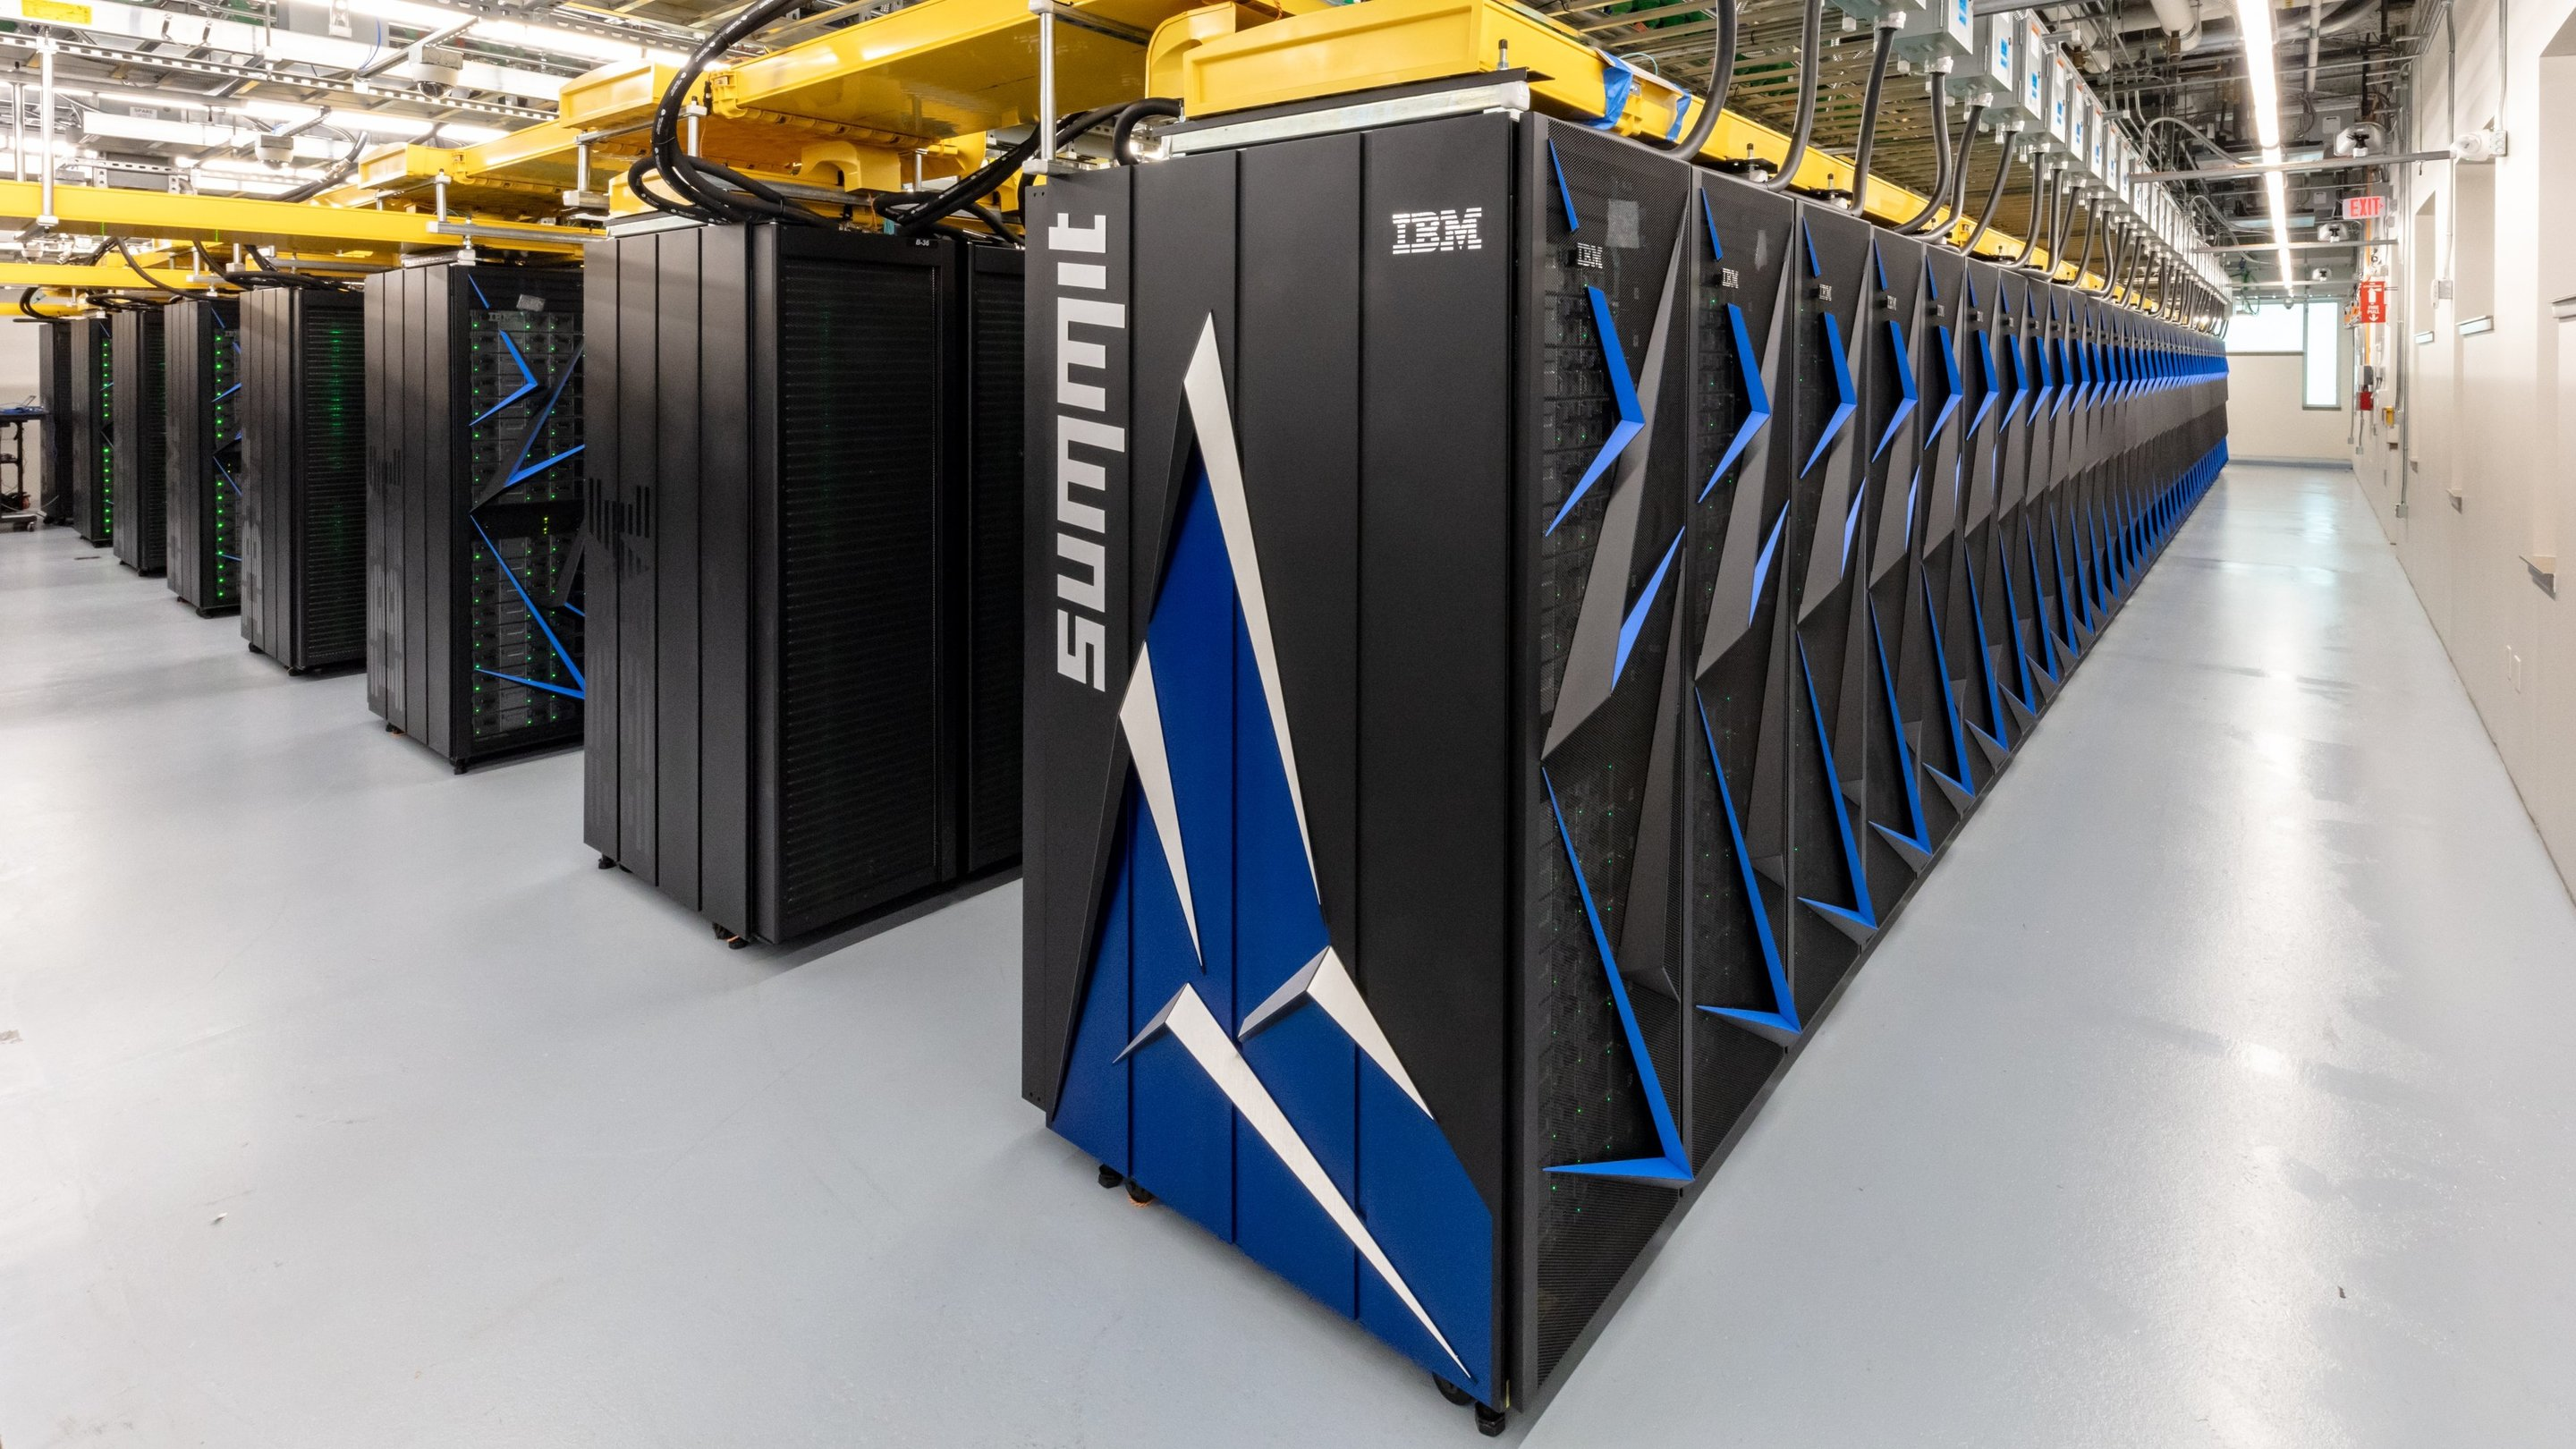
\includegraphics[width=\linewidth]{figures/SummitSC.jpg}
    \caption{The summit supercomputer, currently set to be the worlds fastest supercomputer, taking up the area of two tennis courts. \cite{SummitSC}}
    \label{fig:Summit}
\end{figure}

One crucial area that remains comparatively underdeveloped is software. It will be crucial to provide the missing link between theoretical algorithm and their implementation on a quantum computer. Ideally `quantum programming' should adopt many of the features as its classical counterpart: it should be usable by any person without understanding the details of the hardware being used, while allowing access to the fundamental workings of the computer. However, all programming languages will have to trade off these two features to some degree. Finally it is required to translate the input of the user into a set of instructions that the computer can follow efficiently. This step is called compilation and is crucial to the ability to use computers.

On the other hand, several attempts to  \cite{AlamosIBM2018, Xanadu2018, DK2018, DKBlog, RL2018, JW2018}. However, these documents have often focused on one or two languages. In this guide, we intend to keep a broad overview of the current state of the languages out there. In particular, in the manner of conventional programming guides, we provide many worked examples and problems to aid newcomers to the field. 

%%%%%%%%%%%%%%%
\begin{comment}

There are alraedy several quantum programming languages in place, in this guide we are going to address pyquil by, QISKit by IBM, project Q and Q\#

also citing benchmarking \cite{JW2018}. Our guide is similar to \cite{RL2018} as in we are going to be comparing specific algorithm with different languages, the differences are this and that also all code in jupyter notebooks.

More resources for each programming language

Forest more Resources. pyQUIL other guides and resources. There are already programming guides addressing the use of pyQuil \cite{DK2018} and his blog \cite{DKBlog}.

QISKit more resoruces  \cite{IBM2018}.  \cite{RL2018}. 

Project Q more resources  \cite{RL2018}. 

Q\# more resources (ADD REFERENCES FOR OTHER GUIDES HERE)

REFERENCES for further languages compile this which we briefly describe at the end. \cite{Xanadu2018} \cite{IonQ}

\end{comment}
%%%%%%%%%%%%%


Over the next few years and decades quantum computing is likely to become a reality, eventually becoming accessible to people from a range of disciplines via cloud services. It will be crucial when this becomes the case that people are able to understand how to use these machines in order to harness their applicability to the areas of mathematics, computer science, chemistry and finance. This guide is designed to be an introduction to the science of quantum computers and the current state of the field. Initially we explain in more depth how quantum computers work and their differences to classical computers in \autoref{TheBasics}. Since in the short-term, quantum computers are likely to be noisy, error-prone and limited in scale, we discuss how they can be used in this regime in \autoref{Shortqcomp}. \\

Once the engineering of quantum computers have been improved, then a host of more impressive applications can be demonstrated, which are considered in \autoref{Algorithmsandapplications}. We examine the programming languages that will be able to interface between the algorithms and the quantum computer in \autoref{Programmingquantumcomputer}, and hardware-specific implementations and architectures in \autoref{Implementations}. \\

A more complete description of quantum mechanics is given in \autoref{Advancedtopics} for any interested party. 


%%%%%%%%%%%%%%%%%%%%%%%%%%%%%%%%%%%%%%%
\chapter{Background}
\label{Background}

\epigraph{\textit{Let's put a nice quote here!}}{Andres}

\section{Weird Vector things}\label{TheBasics}


In this section we will attempt to introduce quantum mechanics and its basic unit of information, the qubit, for those with little background in physics. Some knowledge of linear algebra may prove useful but is not necessary.  
In classical computing and information theory the fundamental unit of information is the familiar bit. Every bit is a binary number 0 or 1 that we use to represent false or true, or combine together to encode any information we wish. We can (for reasons that will become clear) represent 
a bit as 2-dimensional vector where,
\begin{equation}
0 = \begin{pmatrix} 1\\ 0 \end{pmatrix},
1 = \begin{pmatrix} 0\\ 1 \end{pmatrix}.
\end{equation}
We can combine single bits in vector form to represent any register of bits,
\begin{equation}
\begin{pmatrix} x_0\\ x_1 \end{pmatrix} \otimes
\begin{pmatrix} y_0\\ y_1 \end{pmatrix}
= \begin{pmatrix} x_0 y_0 \\ x_0 y_1 \\ x_1 y_0 \\ x_1 y_1 \end{pmatrix}.
\end{equation}
This notation captures the relevant information but appears rather unwieldy compared to the equivalent binary or decimal representations.
In this form we write the decimal value 6 as,
\begin{equation}
6_{10} = 110_2 =  \begin{pmatrix} 0\\ 1 \end{pmatrix} \otimes \begin{pmatrix} 0\\ 1 \end{pmatrix} \otimes \begin{pmatrix} 1\\ 0 \end{pmatrix} = \begin{pmatrix} 0 \\ 0 \\ 0 \\ 0 \\ 0 \\ 0 \\ 1 \\ 0 \end{pmatrix}.
\end{equation}
Note that we have a zero in every entry apart from the one corresponding the the decimal 6.
The fundamental operation we can perform on this register is flipping the value of the nth bit i.e. we perform a logical NOT operation $ X \begin{pmatrix} 1\\ 0 \end{pmatrix}  $ to find $ \begin{pmatrix} 0\\ 1 \end{pmatrix} $. 
The matrix X has the form,
\begin{equation}
\begin{pmatrix}
 0 & 1 \\ 1 & 0 
\end{pmatrix}.
\end{equation}
This can be extended to find a matrix that allows us to change any basis state into any other, and therefore we can represent all quantum operations in matrix form. Note also that the not operation is reversible; no information is lost in applying it as many times as we like. This turns out to be a general feature of logical operations in quantum computing.


Adding together numbers in either their binary or decimal form is obvious, however this clearly does not correspond to simple addition in their vector representation. 
\begin{equation}
    6_{10} + 5_{10} = 110_2 + 101_2 \neq  \begin{pmatrix} 0 \\ 0 \\ 0 \\ 0 \\ 0 \\ 0 \\ 1 \\ 0 \end{pmatrix} + \begin{pmatrix} 0 \\ 0 \\ 0 \\ 0 \\ 0 \\ 1 \\ 0 \\ 0 \end{pmatrix}.
\end{equation}
A vector representation of our bits however \textit{should} allow addition and we will now see how to interpret this. Rather than our register being in a definite single \textit{state} corresponding to a single decimal number we can allow superpositions of vectors with each element corresponding to a bit register. For example,
\begin{equation}
    \begin{pmatrix} 0 \\ 1 \\ 0 \\ 0 \end{pmatrix} + \begin{pmatrix} 0 \\ 0 \\ 0 \\ 1  \end{pmatrix},
\end{equation}
is a valid state (however we are now moving away from classical information). This no longer has a clear and unambiguous representation in binary. Furthermore, we can change the signs between vectors and have,
\begin{equation}
    \begin{pmatrix} 0 \\ 1 \\ 0 \\ 0 \end{pmatrix} - \begin{pmatrix} 0 \\ 0 \\ 0 \\ 1  \end{pmatrix}.
\end{equation}
What this represents in information terms is no longer obvious and, more importantly, how can we retrieve information stored in this way? Classically the state of an entire computer is in principle represented by a single string of bits and we can determine each one with certainty. Moving beyond classical information the situation becomes more complicated. If we attempt to measure a superposition of our vectors, asking ``\textit{which state is our register in?}'' we will find $\begin{pmatrix}  0 \\ 1 \\ 0 \\ 0 \end{pmatrix}$ with probability $0.5$ and $\begin{pmatrix}  0 \\ 0 \\ 0 \\ 1 \end{pmatrix}$ with probability 0.5. In order to ensure our probabilities sum to 1 we should normalise our even superposition with a factor of $\frac{1}{\sqrt{2}}$ however this will be ignored for clarity. We can even allow superpositions with more elements i.e. three or more possible outcomes from measurement and factors in front of each vector to adjust the probabilities. To further complicate things we can even allow complex factors in front of our basis vectors, and as it turns out this necessary to fulfil the condition that we can continuously transform any vector into another \cite{hardy2001quantum}. That is to say that there exists a matrix like X introduced above that allows us to move between any states or superpositions thereof. 


So far we have mainly dealt with vectors more complicated than the simple representations of 0 and 1 we introduced earlier. Returning to these we can now introduce the qubit,
\begin{equation}
    \alpha \begin{pmatrix}  1\\ 0 \end{pmatrix} + \beta \begin{pmatrix} 0\\ 1 \end{pmatrix}
\end{equation}
where $\alpha$ and $\beta$ are real or complex number such that $|\alpha|^2 + |\beta|^2 = 1$. This is the reasonable requirement that probabilities should always sum to 1, but encapsulates the principle of superpositions that we measure to find outcomes. In more standard notation we represent vectors in quantum mechanics with a `ket' $|\psi\rangle$. Anything inside the ket is simply a label and can be changed for convenience depending on the situation. For example we traditionally use $\psi$ to denote an arbitrary quantum state with basis vectors in binary i.e.,
\begin{equation}
    |\psi\rangle = \alpha |0\rangle + \beta |1\rangle ,
\end{equation}
is the same state as above in dirac notation. The probability of obtaining the outcome $|1\rangle$ from this state is $|\langle 1|\psi\rangle|^2$ where $\langle 1|$ is known as a `bra,' forming a dirac `bracket' with the state $|\psi\rangle.$ This is nothing more than the inner product of vectors taken to the absolute value squared to ensure we always obtain real and positive probabilities. 

A full model of computation requires more than representations of states and a conceptual method for reading out data. In the next section we will see how to process quantum information in the so-called circuit model. 


A complete mathematical description of quantum mechanics is given in \autoref{Advancedtopics}. 


%%%%%%%%%%%%%%%%%%%%%%%%%%%%%%%%%%%%
\section{The gate model and quantum circuits}

This section briefly reviews the gate model for circuit based quantum computing and discusses the similarities between between digital and quantum computers. The gate model is one of the most popular architectures for quantum computation at the moment. A number of companies such as, \textit{Intel \cite{intelqcomp} IBM \cite{ibmqweb}, Google \cite{googleqai} and Rigetti \cite{rigetti}} are all using the gate model approach for quantum computing. There are other architectures for quantum computing however we think that the gate model is the most similar to digital computers.

Both forms of computation follow the same structure, you start with bits (or qubits), operations are performed on the (qu)bits and then you measure the new values of the (qu)bits. We show an example in \autoref{fig:basicoperation}.

%%%% digital circuit
\begin{figure}[H] 
\centering
\begin{subfigure}[h]{0.4\textwidth}
\begin{align*}
\Qcircuit @C=0.5cm @R=0.7cm
{&\lstick{A} &\multigate{2}{Operation} & \\
&\lstick{B} &\ghost{Operation} & \\
&& &\qw &\lstick{Q} \\}
\end{align*}
\caption{Digital operation}
\label{fig:digitalcirc}
\end{subfigure}
~
%%%% Q circuit
\begin{subfigure}[H]{0.4\textwidth}
\begin{align*}
\Qcircuit @C=0.5cm @R=0.7cm
{&\lstick{A} &\multigate{2}{Operation} &\qw &\lstick{A} \\
&\lstick{B} &\ghost{Operation} &\qw &\lstick{B} \\
&\lstick{Q} &\ghost{Operation} &\qw &\lstick{Q} \\}
\end{align*}
\caption{Quantum operation}
\label{fig:quantumcirc}
\end{subfigure}
\caption{Digital and quantum logic circuits for implementing an arbitrary operation on bits $A, B$ returning value $Q$}
\label{fig:basicoperation}
\end{figure}

One of the main differences between the two figures is that in the quantum circuit the inputs $A \& B$ exist after the operation and the output $Q$ is present before the operation. This is a feature of quantum computing being reversible (unitary).  

One of the requirements for quantum computing to be universal is that we are able to perform any single qubit and a single two qubit gate. Most quantum algorithms make use of a Hadamard gate at the beginning of the computation. 


\begin{figure}[H]
    \begin{align*}
    \Qcircuit @C=0.5cm @R=0.7cm
    {&\lstick{0} &\gate{H} &\qw &\rstick{\frac{0+1}{\sqrt{2}}} \\ 
    &\lstick{A} &\qw &\qw &\rstick{A} }
    \end{align*}
    \caption{Hadamard gate acting on the top qubit and no gate performed on the bottom qubit}
    \label{fig:my_label}
\end{figure}


Multiple qubits gates are of the form, control-\textit{Operation}, one of the most popular two-qubit gates used is the Controlled-NOT. The control means use the value of the first qubit to decide whether or not to perform the operation on the target qubit. 


\begin{figure}[H]
    \begin{align*}
    \Qcircuit @C=0.5cm @R=0.7cm
    {&\lstick{0} &\gate{H} &\qw &\rstick{0 \text{  if  } A=0, \frac{0+1}{\sqrt{2}} \text{  if  } A=1 } \\ 
    &\lstick{A} &\ctrl{-1} &\qw &\rstick{A} }
    \end{align*}
    \caption{Hadamard gate acting on the top qubit and no gate performed on the bottom qubit}
    \label{fig:my_label}
\end{figure}



\subsubsection{Digital logic}

Every digital computing operation can be built up from NAND logic gates \cite{sheffer1913set}. We can call a NAND logic gate a universal gate for computation. The NOR gate is also universal in the same way any computation can be constructed from NOR gates.

\begin{figure}[H]
  \centering
  \begin{subfigure}[h]{0.4\textwidth}
  \centering
  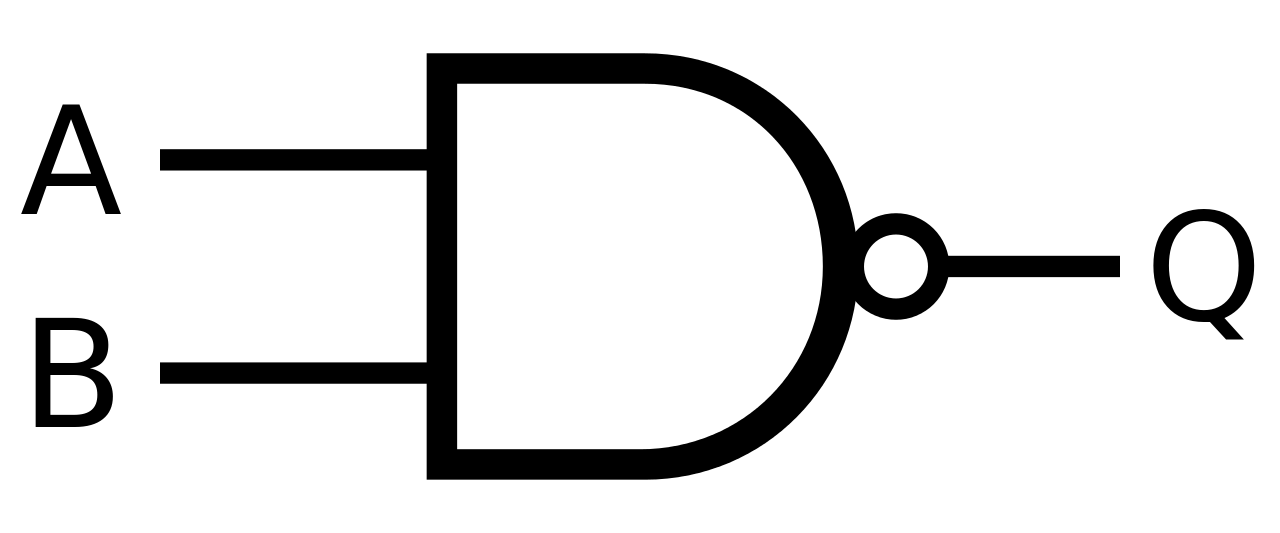
\includegraphics[width=0.7\textwidth]{NAND_ANSI_Labelled_svg.png}
  \caption{The NAND logic gate \cite{nandwiki}.}
  \label{fig:NAND}
\end{subfigure}
~
  \begin{subfigure}[h]{0.4\textwidth}
  \centering
  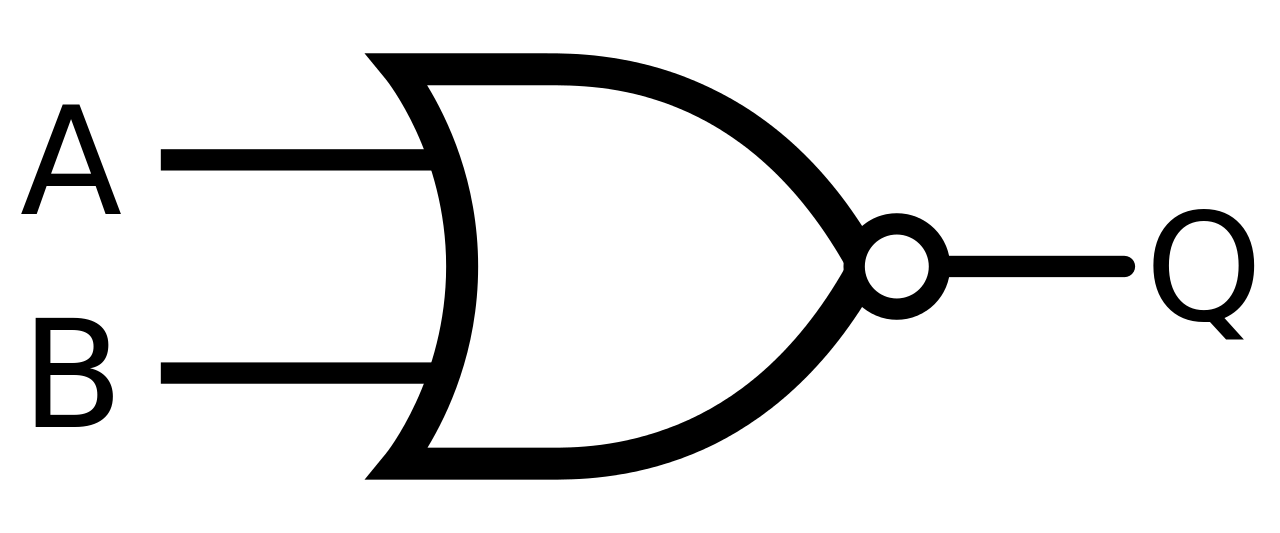
\includegraphics[width=0.7\textwidth]{NOR_ANSI_Labelled_svg.png}
  \caption{The NOR logic gate \cite{norwiki}.}
  \label{fig:NOR}
  \end{subfigure}
\end{figure}

\begin{table}[!htb]
    \caption{Global caption}
    \begin{subtable}{.5\linewidth}
      \centering
        \begin{tabular}{|l|l||l|}
        \hline
        Input A & Input B & Output Q \\ \hline
        0       & 0       & 1       \\ 
        0       & 1       & 0       \\ 
        1       & 0       & 0       \\ 
        1       & 1       & 0       \\
        \hline
    \end{tabular}
    \caption{NOR gate truth table}
    \end{subtable}
    %
    \begin{subtable}{.5\linewidth}
      \centering
        \begin{tabular}{|l|l||l|}
        \hline
        Input A & Input B & Output Q \\ \hline
        0       & 0       & 1       \\ 
        0       & 1       & 1       \\ 
        1       & 0       & 1       \\ 
        1       & 1       & 0       \\
        \hline
    \end{tabular}
    \caption{NAND gate truth table}
    \end{subtable} 
\end{table}


\begin{comment}
reversible logic




%%%%%%%%% circuit 1 
\begin{figure}[h!]
\begin{align*}
\Qcircuit @C=0.5cm @R=0.7cm
{%1
&\lstick{S_1} &\gate{H} &\ctrl{1} &\qw \\
%0
&\lstick{S_0} &\ctrl{-1} &\targ &\qw \\}
\end{align*}
\caption{Schur transform for 2 qubits}
\label{cir:vanilla2}
\end{figure}

\end{comment}

%%%%%%%%%%%%%%%%%%%%%%%%%%%%%%%%%%%%%%%%
\chapter{Quantum Programming Languages}
\label{QPL}

\epigraph{\textit{A new breed of quantum programmer is needed to study and implement quantum software — with a skillset between that of a quantum information theorist and a software engineer.}}{Will Zeng\\ Rigetti Computing \cite{WZ2017}}

%%%%%%%%%%%%%%%%%%%%%%%%%%%%%%%%%%
%%%%%%%%%%%%%%%%%%%%%%%%%%%%%%%%%%

I think here we should thoroughly explain the syntax of each language with a basic example implementation.  with examples (not Deutsch cause we haven't explained it yet). I propose I super simple example, like generating a superposition state and performing some measurements.

For each language need to talk about the following:
\begin{itemize}
\item How is the program structured? (E.g. as a quantum processor/subprogram to regular programming language)
\item Qubit, Ancilla bits, Classical bits
\item How are gates applied?
\item How are measurements handled?
\item Available libraries
\item Available for which operating systems
\item Use case of language and future of language
\item Support available
\item Flexibility of language (hardware, simulation, cost estimator, etc.)
\end{itemize} 

%%%%%%%%%%%%%%%%
%%%%%%%%%%%%%%%%
%%%%%%%%%%%%%%%%
%%%%%%%%%%%%%%%%
\section{Rigetti - pyQuil}
%%%%%%%%%%%%%%%%
%%%%%%%%%%%%%%%%
%%%%%%%%%%%%%%%%
%%%%%%%%%%%%%%%%

In this section we address the main features of the programming language by Rigetti and the description of its syntax with a simple example.

pyQuil is the Python based programming language created by Rigetti \cite{pyQuilDoc} as part of their quantum programming toolkit for their hardware. This consists of
\begin{itemize}
    \item \textbf{Forest} - Rigetti's entire quantum programming toolkit. 
    \item \textbf{Quil} – Quantum Instruction Language which is assembly-like as it lists the gates to apply. Acts as an intermediate step between pyQuil and the actual instructions that will go to the quantum computer.
    \item \textbf{pyQuil} - Open source Python library. The user writes their code in pyQuil and this gets translated to Quil.
    \item \textbf{QVM} - Rigetti's Quantum Virtual Machine which runs simulations of up to 26 qubits, an API key is required to access this.
    \item \textbf{QPU} – Quantum Processing Unit, Rigetti's actual chip with 19 qubits which requires special access.
    \item \textbf{Grove} - Open source Python library containing quantum algorithms developed with pyQuil. 
\end{itemize}

\begin{figure}[H]
    \centering
    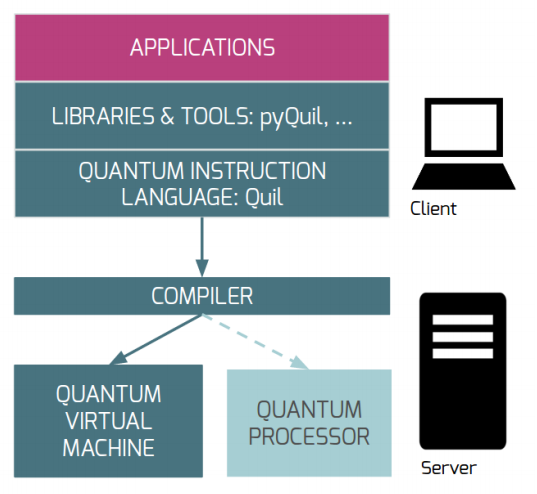
\includegraphics[width=0.5\textwidth]{Forest_structure.PNG}
    \caption{The structure of Forest. Figure taken from \cite{Rigetti2016} - possibly need to create our own}
    \label{fig:my_label}
\end{figure}

A program would be written in pyQuil which gets translated to Quil. If the program is being run on the QVM, it is generally not necessary to decompose the Quil instructions further since the code is being run on a simulator and everything comes down to mathematical operations. If the program is to be run on the QPU, a compiler will break down the Quil instructions into quantum gates which can be executed on the actual chip. This is necessary because QPUs currently have a more limited gate set due to the technology used to create the chip. For example if you would like to perform a controlled-NOT gate, this may have to be broken down into the elementary gates for the specific chip architecture.  

Quil has been designed with the idea in mind that near term quantum computers will act as co-processors along with classical processors. It can execute quantum programs with classical control. pyQuil is more of a high-level language, hence in the guide we will be focusing on this rather than Quil.   

%%%%%%%%%%%%%%%
%%%%%%%%%%%%%%%
\begin{comment}

The Rigetti-Forest toolkit \cite{Rigetti2016} for hybrid classical-quantum computing uses the language called Quil. The python library called pyQuil allows us to run simulations in their Quantum Virtual Machine (QVM) which allows the simulation up to 26 qubits, and to run simulations on their Quantum Processor Unit (QPU) which is the physical device called 19Q Acorn which have 20 physical qubits, of which 18 are logical. They recently made available a ~100 pages pyQuil documentation \cite{pyQuilDoc} with examples and exercises to be implemented whether in the QVM or QPU. Access to the QVM can be granted to everyone by registering in their website (they send you an API key right away).

\end{comment}

%%%%%%%%%%%%%
%%%%%%%%%%%%%
%%%%%%%%%%%%%%%%%%%%%%%%%%%%%%%%%%%%%%%%%
%%%%%%%%%%%%%%%%%%%%%%%%%%%%%%%%%%%%%%%%%
%%%%%%%%%%%%%%%%%%%%%%%%%%%%%%%%%%%%%%%%%
\subsection*{Quantum Programs with pyQuil} 
\label{Quantum Programs with pyQuil}
%%%%%%%%%%%%%%%%%%%%%%%%%%%%%%%%%%%%%%%%%
%%%%%%%%%%%%%%%%%%%%%%%%%%%%%%%%%%%%%%%%%
%%%%%%%%%%%%%%%%%%%%%%%%%%%%%%%%%%%%%%%%%

Quantum algorithms require the implementation the three computational stages. We first need to initialise the state in a state of the form $\ket{00...0}$, we then need to apply gates in order to obtain a target state of interest and finally, we perform measurements in the computational basis. Let us see how to address these stages with the following specific example.

%%%%%%%%%%%% title= Example 1
\begin{tcolorbox}[standard jigsaw,
    opacityback=0,  % this works only in combination with the key "standard jigsaw"
    boxrule=0.5pt,label={example1}]
    {\bf Example 1}
    \tcbline
    Generating the one-qubit pure state 
    \begin{align*}
    \ket{\psi\left(\phi\right)}=\frac{1}{\sqrt{2}}\left(\ket{0}+e^{i\phi}\ket{1}\right),
    \end{align*}
    by applying gates to the initial state $\ket{0}$ and performing measurements.
\end{tcolorbox}
%%%%%%%%%%%%%%%
Starting with the one-qubit state $\ket{0}$, we can generate the superposition with a Hadamard gate, and we then can add the desired phase with a gate of the form $here$. Finally, we consider projective measurements. We remark here however, that these steps can be implemented in any programming language that handles linear algebra.  We can do it in python with the Python library Numpy in the following way \autoref{lst:ExamplePython}.

%\columnbreak
%%%%%%%%%%%%%%%%%
\begin{lstlisting}[language=Python,caption={Example with python only},label={lst:ExamplePython},frame=single] 
import numpy as np
# State initialisation
state0=np.array([[1],[0]])
# State manipulation
H=(1/np.sqrt(2))*np.array([[1,1],[1,-1]])
state1=np.dot(H,state0)
phi=np.pi/2
PHASE=np.array([[1,0],[0,np.exp(1j*phi)]])
state2=np.dot(PHASE,state1)
# Measurement: defining projectors P0,P1
ket0=np.array([[1],[0]])
ket1=np.array([[0],[1]])
P0=np.dot(ket0,ket0.T)
P1=np.dot(ket1,ket1.T)
# Probability of obtaining outcome 0
prob0=np.trace(np.dot(P0,np.dot(state2,np.conj(state2).T)))
# Probability of obtaining outcome 1
prob1=np.trace(np.dot(P1,np.dot(state2,np.conj(state2).T)))
\end{lstlisting}
%%%%%%%%%%%%%%%%
However, this is local, and we are running this computation in our standard computers and therefore is a classical simulation of a quantum computation.

We would like to implement this in a real quantum computer, and this is where Rigetti comes in. We need further software to manipulate real QPUs, and therefore cannot be as straightforward as our previous code. but we are using the QVM.

%\columnbreak

{\bf 0. Libraries:} The connection and qubit initialisation of our qubits is given by:
\begin{lstlisting}[language=Python]
from pyquil.quil  import Program 
from pyquil.api   import QVMConnection 
from pyquil.gates import I,X,Z,Y,H,PHASE
import numpy as np
\end{lstlisting}

{\bf 1. Initialisation:} The systems has been initialised into a state of $n$
 qubits in the $|00...0>$ state. Of course both the qvm and qpu are limited by this and that respectively.\\ 
 
 the other point is that this is a lst of instructions and the actual computation has not taken place, and we need to invoke the command run to do it.\\
\begin{lstlisting}[language=Python,firstnumber=5] 
# Invoking and renaming
qvm=QVMConnection()
p=Program()
\end{lstlisting} % numbers=none 
 
 %%%%%%%%%%%%%%%%%%%%%%%%%%%%%
 {\bf 2. Gate implementation:} So far we have only covered initialisation, now we need to consider state manipulation. The way that gates are being called is as follows:
 %%%%%%%%%%%%%%%%%
\begin{lstlisting}[language=Python,firstnumber=8]
# Gate implementation
p.inst(H(0))
theta=np.pi/2
\end{lstlisting}
%%%%%%%%%%%%%%%%
 by considering the object program which we have renamed as p with the methd isnt we apply fro left to right in order of application and inside parenthesis the qubit which is acting upon the qubits are listed from $0,1,...n$. For instance applying gates this and that. The complete set of gates can be found in HERE.\\
 
%%%%%%%%%%%%%%%%%%%%%
{\bf 3. Measurement:} Yadda describing 
\begin{lstlisting}[language=Python]
# Measurement
p.measure(0,0)
p.measure(1,1)
\end{lstlisting}
 
%%%%%%%%%%%%
{\bf 4. Run:} So far this is only a list, now finally we run the program with the command.
\begin{lstlisting}[language=Python]
# Running the program
cr=[]
results=qvm.run(p,cr,4)
print(results)
\end{lstlisting}
So in full our program looks like this \autoref{lst:ExampleQVM}.
%%%%%%%%%%%%%%%%%
\begin{lstlisting}[language=Python,caption={Example algorithm implemented with pyQuil.},label={lst:ExampleQVM},frame=single] 
from pyquil.quil  import Program 
from pyquil.api   import QVMConnection 
from pyquil.gates import H,PHASE
import numpy as np
# Invoking and renaming
qvm=QVMConnection()
p=Program()
# Gate implementation
p.inst(H(0))
theta=np.pi/2
p.inst(PHASE(theta,0))
# Measurement
p.measure(0,0)
p.measure(1,1)
# Running the program
cr=[]
results=qvm.run(p,cr,4)
print(results)
\end{lstlisting}

%In this section we address the main features of the programming language by (QISKit company) and the description of its syntax with a simple example.

%%%%%%%%%%%%%%%%%%%%%%%%%%%%
\section{IBM - QISKit}
%%%%%%%%%%%%%%%%%%%%%%%%%%%%

IBM has launched the IBM Q experience that consists of a development environment called QISKit, a higher-level gate-building software development kit (SDK) that allows users to compose their own quantum algorithms, and OpenQASM, a low level quantum assembly language to realise the gates at the quantum prosessing unit (QPU). The devices used to perform the simulation and computation are based on a superconducting charge qubit implementation, which can be found described in more detail in \autoref{Implementations}. \\
\indent There is ample space for development of algorithms in this environment as the visual arrays provide a clear structure to those familiar with quantum computation. The composer also displays the code on which it operates so that users interested in further development have the opportunity to learn how to code their own gates in OpenQASM as well as QISKit. The associated documentation which is linked on the IBM Q website provides more detail to the structure \cite{coles2018quantum}. \\
\indent The architectures (physical or virtual) that the user can execute their quantum algorithms on are easily accessible via the IBM Q Experience web page, and can be seen in \autoref{fig:ibmsite}. IBM recently published a report detailing their state-of-the-art prototype 50 qubit chip in the 2017 IEEE ICRC conference \cite{ibm50}.\\

The current state of IBM's stack, from top to bottom consists of the following elements:

\begin{itemize}
    \item \textbf{QISKit} - IBM's open source quantum library for usage in the high level language Python. 
    \item \textbf{QISKit ACQUA} - IBM's open source, modular Algorithms and Circuits for Quantum Applications library for usage in the high level language Python. The modules in this library as specifically targeted towards industry professionals in the research areas of Chemistry, artificial intelligence and optomization. 
    \item \textbf{OpenQASM} – IBM's low-level Quantum Assembly Language which interprets commands and functions from QISKit and translates them into microwave pulses for use on the physical architecture (superconducting qubits). Acts as an intermediate step between QISKit and the actual instructions that will go to the quantum computer.
    \item \textbf{QPU} - IBM has multiple physical architectures for running quantum algorithms. These include 3, 4, 5 and 16 qubit devices accessible via an API provided when you create an account with the IBM Experience, and larger 20 qubit devices that are available via membership to the IMB Q Network (hubs, partner institutions etc).
    \item \textbf{Q QASM Simulator} - IBM's Quantum Virtual Machine which runs simulations of up to 32 qubits, an API key is required to access this.
\end{itemize}
%%%%%%%%%%%%%%%%%%
\begin{figure}[h!]
\centering
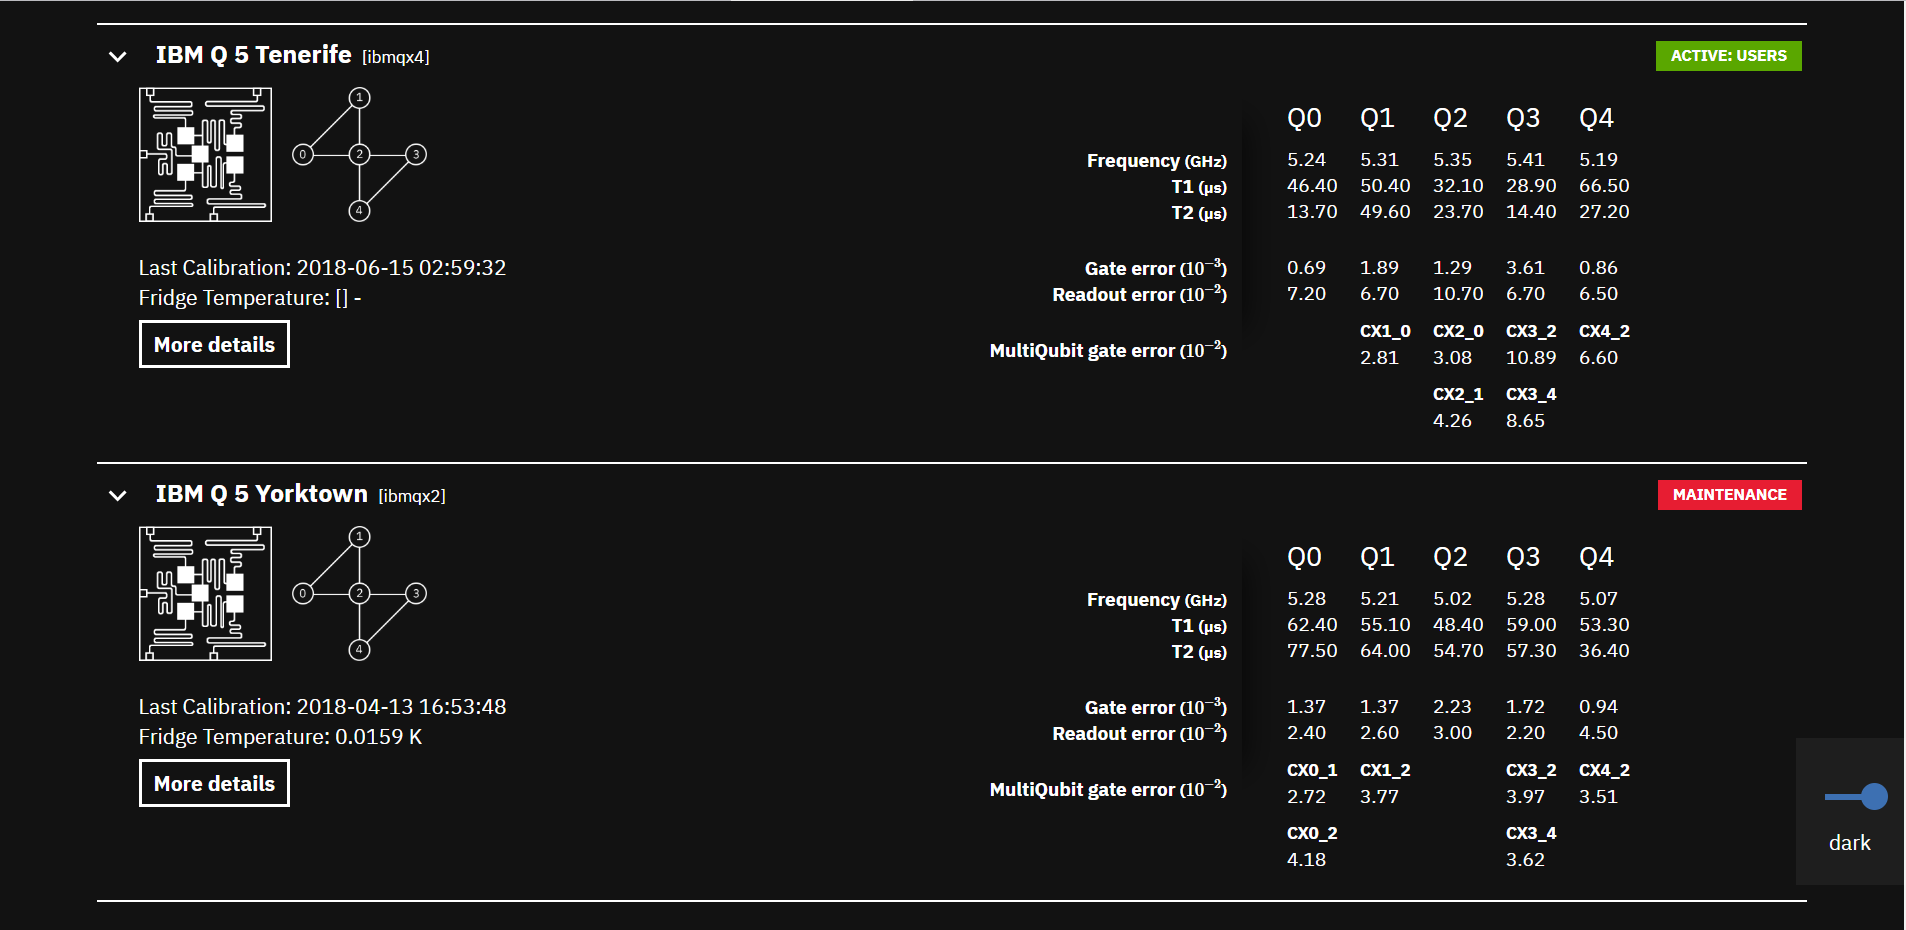
\includegraphics[width=\textwidth]{IBMq_1}
\caption{The description of the devices used for the IBM Q suite (to be updated closer to submission). Cooling refrigerator temperature along with the update structure is presented. A useful live display feed allows users to track both the physical and computational side of their own algorithms made on the composer.}
\label{fig:ibmsite}
\end{figure}

%%%%%%%%%%%%%%%%%%%%%%%%%%%%%%%%%%%%%%%%%
%\subsection{QISKit General Description}
%%%%%%%%%%%%%%%%%%%%%%%%%%%%%%%%%%%%%%%%%

%%%%%%%%%%%%%%%%%%%%%%%%%%%%%%%%%%%%%%%%%
\subsection*{Quantum Programs with QISKit}
%%%%%%%%%%%%%%%%%%%%%%%%%%%%%%%%%%%%%%%%%

The first basic example of QISKit will be to generate a single qubit superposition, $\ket{\psi}=\frac{1}{\sqrt{2}} \left(\ket{0}+e^{i\phi}\ket{1}\right)$, beginning with the all qubits in the state $\ket{0}$. We will focus on the cases of $\phi=0$ and $\phi = \pi$. These can be broken down into the action of the Hadamard operator on $\ket{0}$ and the Hadamard operator followed by the Z Pauli gate. These actions are written in \autoref{eq:H1} and \autoref{eq:ZH}, respectively.

\begin{equation}
    H\ket{0}=\frac{1}{\sqrt{2}}\left(\ket{0}+\ket{1}\right)
    \label{eq:H1}
\end{equation}
\begin{equation}
    ZH\ket{0}=\frac{1}{\sqrt{2}}\left(\ket{0}-\ket{1}\right)

    \label{eq:ZH}
\end{equation} 
We can simulate both of these actions on the composer in the IBM Q experience, or use experiment tokens to run the program on the processor IBM provides (referred to as ibmqx4) as seen in \autoref{fig:ZH}. 

\begin{figure}[h!]
    \centering
    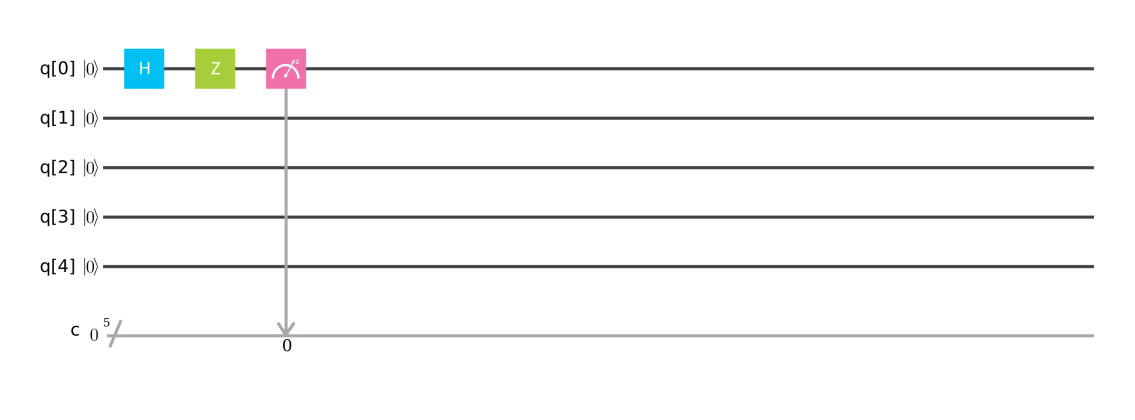
\includegraphics[width=\textwidth]{ZHcodecomposer}
    \caption{The composer view of the code that we can use to simulate the generation of $ZH\ket{0}=\frac{1}{\sqrt{2}}\left(\ket{0}-\ket{1}\right)$.}
    \label{fig:ZH}
\end{figure}

Though the composer is a useful place to get started with your own simulations of basic gate operations, it doesn't give us a an opportunity to truly experiment with the hardware at a deeper level. To do this, we need to start experimenting with the QISKit language itself.

\begin{figure}
    \centering
    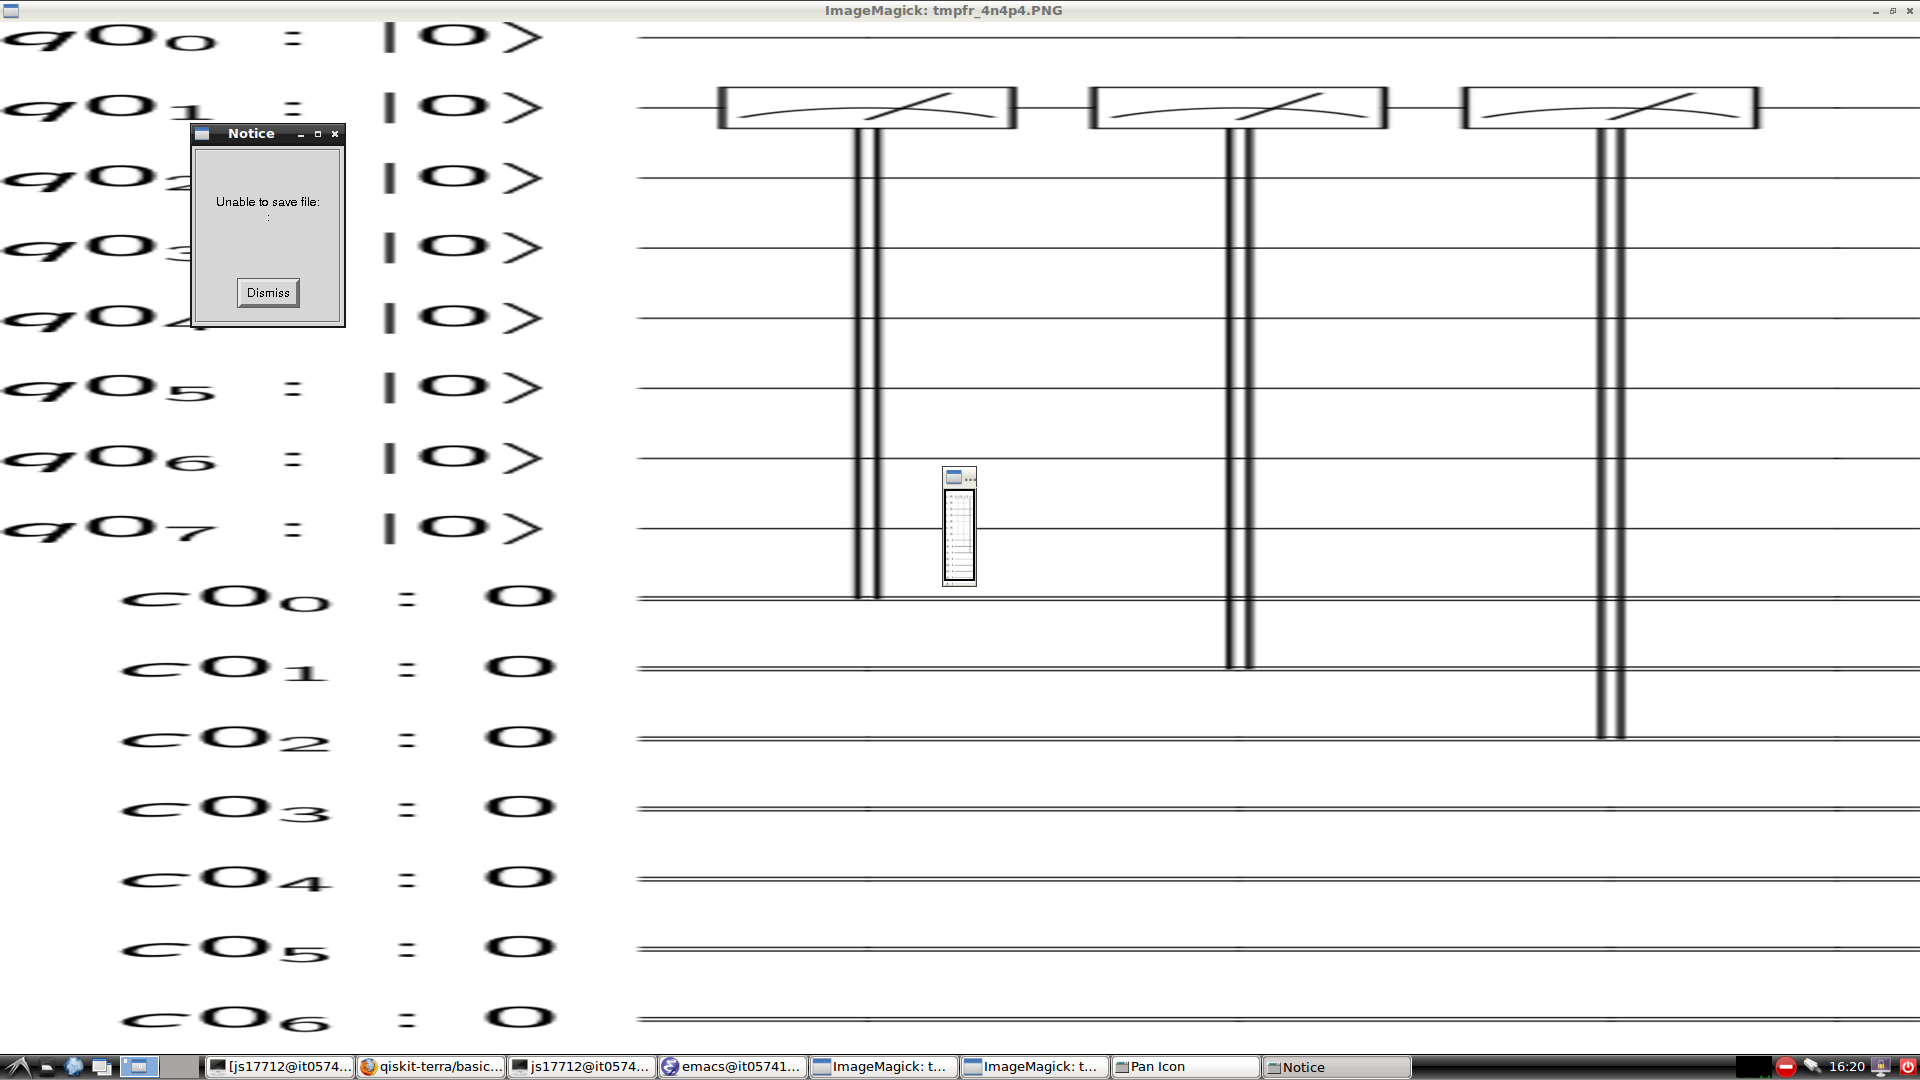
\includegraphics{the_qanswer.png}
    \caption{Caption}
    \label{fig:my_label}
\end{figure}

Consider the previous example illustrated by the gate composer in \ref{fig:ZH}. This relatively simple example can be expanded upon in QISKit via the generation and measurement of a Bell state, described by \autoref{eq:BS}

\begin{equation}
    \ket{\psi}=\frac{1}{\sqrt{2}}\left(\ket{01}+\ket{10}\right)
    \label{eq:BS}
\end{equation} 

To create this state, and measure it on IBM's Q QASM Simulator, the follwoing code can be utilised:
\newpage

\begin{lstlisting}[language=Python,caption={Example algorithm implemented with QISKit.},label={lst:ExampleQQASM},frame=single] 
# Program written using QISKit to demonstrate the way in which to create an equal weighted
# superposition of states in the computational basis, and then simulate the measurement
# on IBM's Q QASM simulator

# Import relevant library functions from QISKit
from qiskit import ClassicalRegister, QuantumRegister, QuantumCircuit
from qiskit import available_backends, execute

# Initiate quantum registers for gate execution, and classical registers for measurements
q = QuantumRegister(2)
c = ClassicalRegister(2)
qc = QuantumCircuit(q, c)

# Preform a Hadamard on the qubit in the quantum register to create a superposition
qc.h(q[0])
# Preform a controlled-not operation between the first and second qubits in the register
qc.cx(q[0], q[1])
# Preform an X-pauli on the second qubit in the register
qc.x(q[1])
# Measure the superposition
qc.measure(q, c)

# Check simulation backends
print("Local backends: ", available_backends({'local': True}))

# Submit the job to the Q QASM Simulator (Up to 32 Qubits)
job_sim = execute(qc, "local_qasm_simulator")
# Fetch result
sim_result = job_sim.result()

#Print out the simulation measuement basis and corresponding counts
print("simulation: ", sim_result)
print(sim_result.get_counts(qc))
\end{lstlisting}

When ran, the output produced is as follows:

\begin{lstlisting}[language=Python,caption={Bell State generation and measurement output.},label={lst:ExampleQQASMoutput},frame=single] 
Local backends:  ['local_qasm_simulator', 'local_statevector_simulator', 'local_unitary_simulator']
simulation:  COMPLETED
{'01': 513, '10': 511}
\end{lstlisting}

Here, the back end in selected in line 1, completion confirmation is shown in line 2, and the measurement basis and counts are shown in line 3, illustrating that indeed the Bell State specified in \ref{eq:BS} has been generated, and measured. 
\newpage


%%%%%%%%%%%%%%%%%%%
%%%%%%%%%%%%%%%%%%%
\section{ProjectQ}

ProjectQ is an open source Python based language. ProjectQ can run on a local simulator - your computer. But there is also an option to connect to the IBM back-end to run code on their simulator or chips, and this may be extended to other hardware in the future as well. This makes ProjectQ a general quantum programming language that is not platform specific unlike pyQuil, QISKit and Q\#.  

\begin{figure}[H]
    \centering
    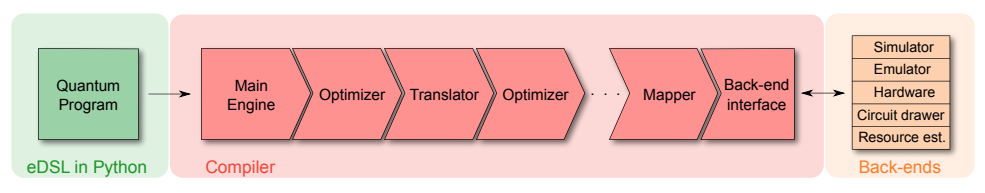
\includegraphics[width=\textwidth]{projectq_structure.PNG}
    \caption{Structure of ProjectQ. Taken from \cite{projectq2018}, will make own diagram and possibly simplify.}
\end{figure}

ProjectQ is one of the more flexible quantum programming languages available in terms of the types of operations, compilers and back-ends that are available. Many of the typical gates that are used in quantum algorithms are already built in, and user defined gates that are either just matrices or based on mathematical operations are relatively simple to implement. 

The compiler is designed to have a modular structure, so the user can pick and choose the level of optimisation required. 

% Note: This section is not finished! I will complete the compiler paragraph and discuss the different back-ends etc. 

%%%%%%%%%%%%%%%%%%%%%%%%%%%%%%%%%%%%%%%%%%%
\subsection*{Quantum Programs with ProjectQ}
%%%%%%%%%%%%%%%%%%%%%%%%%%%%%%%%%%%%%%%%%%%

% I may add another example to this section since it is quite short. Or do things need explaining in more detail?

We will now do a simple demonstration in ProjectQ to create the superposition $\frac{\ket{0}+\ket{1}}{\sqrt{2}}$. 

\lstinputlisting[language=Python]{code/ProjectQ/superpos_projectq.py}

The first thing to do is to set up the back-end that the program will be run on. This is done by calling \texttt{MainEngine} which has the local simulator as the default back-end, this can also be set up to be the IBM back-end or something else such as a resource estimator.

Qubits can now be allocated, either individually (as shown above) or as a register, from the \texttt{engine}. The syntax to do an operation is  \texttt{Gate | Qubits}. Finally the gates are sent to the compiler by use of the \texttt{flush} command. And if you wish to display the result, the qubit can be converted to type integer after measurement.


\newpage
%%%%%%%%%%%%%%
%%%%%%%%%%%%%%
\section{Q\#}
%%%%%%%%%%%%%%
%%%%%%%%%%%%%%
One of the languages that is strongly quantum platform independent is Q\#. It is being developed by Microsoft and very roughly based on their classical languages C\# and F\#. It is, however, not just a library, but designed to be its own language. Q\# is developed to be a high-level quantum programming language. Though it still allows the basic single qubit operations, it also provides a more advanced library and allows user-defined ``operations" which can be used to structure more complicated programs. The programming language should be platform independent to allow users to write programs now for quantum computers available in the future. Currently it runs on a simulator (either on your local computer or Azure, a Microsoft cloud computing service) or a cost estimator (trace simulator) which approximates qubit and gate requirements for the program. \\
The concept behind the language is that the quantum computer is treated like a coprocessor: like GPU is a graphical coprocessor, a QPU is the quantum one. This means that a program using the QPU requires a driver program, which controls the main processor (CPU) and which then calls on a subprogram controlling the QPU. The QPU program in this case will be written in Q\#, whereas the driver program can be written in not just C\# or F\#, but any language supporting the .NET framework. In this programming guide the driver programs are written in C\#, but you could easily change this if you are more comfortable with another language.\\
As Q\# is dependent on the .NET framework, it is currently only available for Windows computers. The easiest way to get started is probably by programming with Visual Studio. Tutorials for installing this API and Q\# can be found online. \\
Q\# comes with a standard library which is divided into two sections: The basic building blocks of the language, such as the qubit and measurements representations and the operations given above, are part of the so-called prelude. The prelude is dependent on the target machine, e.g. a simulator.  The second part, called the canon, is machine independent and built on the elements that form the prelude. It gives implementations of various quantum algorithms such as a quantum Fourier transform and a phase estimation.  

\paragraph{Basic building blocks} There are several primitive types specific to Q\# and an overview of these is given in table \ref{table:PrimTypeQsharp}. The first five are analogous to types in classical programming languages, e.g. C\#. The others are more quantum programming specific. \\
It is also possible to create arrays, e.g. a \texttt{Qubit[]} or an \texttt{Int[][]}. Tuples, so e.g. (a, b, c), are also used. a, b and c could be of different types and tuples can be quite useful in returning multiple values from an operation. You can also define your own types, but they must be based on the primitive types.\\
Another thing a Q\# programmer has to keep in mind, is that variables are normally immutable. Values are assigned with a \texttt{let} statement and they cannot be changed afterwards. To allow changing the value of a variable one can use the \texttt{mutable} keyword when assigning a value to a variable. Changing the variable is then done with the \texttt{set} statement.\\
Qubits are maybe the most important resource in a quantum program. You cannot assign a value to a \texttt{Qubit}, but you can measure it and then apply operations to change it to the value you want. The default value of a \texttt{Qubit} is $\ket{0}$, i.e. the computational \texttt{Zero} state, and it is generally good practice to reset a used \texttt{Qubit} to this before releasing it.\\
The easiest way to use actually use \texttt{Qubit}s is to write a \texttt{using} statement, e.g. \texttt{using (qubits = Qubit[2])\{<any code using these qubits>\}}.

\begin{table}[!htb]
      \centering
        \begin{tabular}{|l|l|}
        \hline
        Type    & Values \\ 
        \hline
        \texttt{Int}     & 64-bit signed integer \\
        \texttt{Double}  & double-precision floating-point number \\
        \texttt{Bool}    & Boolean value (\texttt{true} or \texttt{false}) \\
        \texttt{String}  & Unicode sequence, used to pass messages to classical driver program\\
        \texttt{Range}   & sequence of integers\\
        \texttt{Qubit}   & qubit\\
        \texttt{Result}  & outcome of measurement (\texttt{One} or \texttt{Zero})\\
        \texttt{Pauli}   & elements of the Pauli group (\texttt{PauliI}, \texttt{PauliX}, \texttt{PauliY} or \texttt{PauliZ})\\
        \hline
    \end{tabular}
    \caption{Primitive types in Q\#}
    \label{table:PrimTypeQsharp}
\end{table}

%%%%%%%%%%%%%%%%%%%%%%%%%%%%%%%%%%%%%%%%%
\subsection*{Quantum Programs with Q\#}
%%%%%%%%%%%%%%%%%%%%%%%%%%%%%%%%%%%%%%%%%
Q\# programs require two main bits of code: a ``classical" driver program and the quantum program. The driver program here is in C\#, but as mentioned in the previous section this could be another language. It must use two namespaces: \texttt{Microsoft.Quantum.Simulation.Core} and \\ \texttt{Microsoft.Quantum.Simulation.Simulators}. Next you want to define the namespace you want to work in: in this case Quantum.Superposition, which will be shared by your driver and your quantum program.\\
Then you start your driver program like you would any regular program. In C\# you create a class and the entry point for the program is your \texttt{static void Main(string[] args)} method.\\
As we do not have an actual QPU, we are using a simulator. To create an instance of the simulator in your program you can use a \texttt{using} block. This creates the simulator instance and ensures it is disposed of when the block ends.\\
In the "using" block you can then call on the quantum operation defined in your quantum subprograms. In this case that will be the operation "Superposition". The operation is actually run with the method \texttt{Run(<QuantumSimulator>, arg1, arg2, ...)}, where the \texttt{arg} arguments are any potential arguments passed to the quantum operation. In this simple example the quantum operation does not take any arguments so we are only passing the Quantumsimulator \texttt{sim} to \texttt{Run}. Finally, we want to actually get the outcome of the quantum operation, which we get by adding \texttt{.Result} to the end.\\
Then the rest of the driver program can be completely classical again, with the exception that the objects returned can be specific quantum types.\\


\begin{lstlisting}[language=Csharp,caption={Starting a driver program for Q\#},label={lst:C\#driverSimple}] 
using Microsoft.Quantum.Simulation.Core;
using Microsoft.Quantum.Simulation.Simulators;

namespace Quantum.Superposition{

    class Driver{
        static void Main(string[] args){

            using (var sim = new QuantumSimulator()) {
                Result outcome = Superposition.Run(sim).Result;
                System.Console.WriteLine
                        ($"Measuring equal superposition state gave outcome {outcome}.");
            }

            System.Console.WriteLine("Press any key to continue...");
            System.Console.ReadKey();
        }
    }
}
\end{lstlisting}

To specify the quantum operation you need to write Q\# code. Again, you start by defining the namespace we are working in (\texttt{Quantum.Superposition}). Next there are two namespaces you will need to use, which are specified with the keyword \texttt{open} (similar to \texttt{using} in C\#): \\ \texttt{Microsoft.Quantum.Primitive} and \texttt{Microsoft.Quantum.Canon}.\\
New operations are defined with the keyword \texttt{operation} and the arguments taken and the return value is specified here in the form \texttt{operation OperationName (arg1: type1, arg2: type2, ...) : (returnType)}.
Inside the operation you define the actual steps to take in the \texttt{body} block. \\
Here we are defining a mutable variable res. It is assigned the value \texttt{Zero}, which is of type \texttt{Result}. This variable will be used to return the outcome of the quantum operation. Next, a \texttt{Qubit} array containing one \texttt{Qubit} is created and after applying a Hadamard (\texttt{H}) gate the \texttt{Qubit} will be in state $\frac{\ket{0}+\ket{1}}{2}$. Then the \texttt{Qubit} is measured (\texttt{M}) and afterwards returned to the $\ket{0}$ state. The measurement outcome is then returned to the driver program. \\
One thing to note here is that we needed to define the variable \texttt{res} outside the \texttt{using} block, as any variables defined in the block are local only to the \texttt{using} block. We cannot use the return statement inside the \texttt{using} block either, so we needed to use a variable local to the whole \texttt{body} block to return a value from the operation.\\

\begin{lstlisting}[language=Qsharp,caption={A simple program in Q\# creating and measuring an equal superposition.},label={lst:Q\#Simple}]
namespace Quantum.Superposition{

    open Microsoft.Quantum.Primitive;
    open Microsoft.Quantum.Canon;

    operation Superposition() : (Result){

      body{

        mutable res = Zero;

	    // create a qubit reqister
	    using (reg = Qubit[1]){
	      // Apply the Hadamard gate to your qubit to create an equal superposition
          H(reg[0]);

	      // Measure the qubit in superposition
	      set res = M(reg[0]);

	      // Reset the qubit to its clean |0> state
	      if (res == One){
	        X(reg[0]);
	      }
	    }

      return res;
            
      }
    }
}
\end{lstlisting}

%%%%%%%%%%%%%%%%%%%%%%%%%%%
\section{Further languages}
%%%%%%%%%%%%%%%%%%%%%%%%%%%

TODO: short overview of other languages available.

Here is the list of some other languages also mentioned in \cite{RL2018}. Are there more?
\begin{itemize}
    \item Strawberry Fields for CV by Xanadu \cite{Xanadu2018}
    \item IonQ \cite{IonQ}
    \item Is Quantum Developer Kit the same QISKit?
    \item others?
\end{itemize}

%%%%%%%%%%%%%%%%%%%%%%%%%%%
\section{Comparison Discussion?}
%%%%%%%%%%%%%%%%%%%%%%%%%%%

I think we should talk about the pros and cons of each language, to give the readers an idea of which one better fits their needs?
\begin{itemize}
    \item {\bf Language-based?} Three of them are python-based, Q\# is not python-based
    \item {\bf Open source?} all of them are open source (which is good, I think)
    \item {\bf QPU?} pyquil, qiskit, project Q have access to QPU, Q\#? (could anyone confirm this?) although u need to request access to this.
    \item {\bf QVM?} about QVM do they all offer QVM services?
    \item {\bf how beginner-friendly is the syntax?}
    \item {\bf particular conveniences} easy to implement oracles? qft? what other conveniences?
    \item what other general characteristics should we highlight?
\end{itemize}


\newpage
%%%%%%%%%%%%%%%%%%%
\section{Exercises}
%%%%%%%%%%%%%%%%%%%

Implement the following examples in the language of your choice.

%%%%%%%%%%%%%%%%
\begin{tcolorbox}[standard jigsaw,
    opacityback=0,  % this works only in combination with the key "standard jigsaw"
    boxrule=0.5pt]
    {\bf Exercise 1:  Arbitrary one-qubit pure state}
    \tcbline
    Generating an one-qubit state of the form:
    \begin{align*}
    \ket{\psi\left(\phi,\theta\right)}=\frac{1}{\sqrt{2}}\left(\cos{\theta}\ket{0}+e^{i\phi}\sin{\theta}\ket{1}\right),
    \end{align*}
    by applying gates to the initial state $\ket{0}$ and performing measurements in the computational basis. What is the probability of obtaining outcome $0$ for a given $\ket{\psi\left(\phi,\theta\right)}$?
\end{tcolorbox}
%%%%%%%%%%%%%%%%

List of further exercises?
\begin{itemize}
    \item Creating a Bell state
\end{itemize}

Even though they are not algorithms perse, perhaps itd be nice to leave as an exercise one of the following?

Using the Bell state as a resource for one of these protocols?
\begin{itemize}
    \item Teleportation?
    \item Super Dense coding?
\end{itemize}






%%%%%%%%%%%%%%%%%%%%%%%%%%%%%%%%%%%%%%%%%%%%%
%%%%%%%%%%%%%%%%%%%%%%%%%%%%%%%%%%%%%
\chapter{Short term quantum computing}
\label{Shortqcomp}

\epigraph{\textit{Let's put a nice quote here! A Quantum supremacy quote?}}{Andres} % a Q supreacy quote

In this section we aim to give a comprehensive overview of quantum computing platforms which are currently available and discuss the near-term advantages that these platforms can bring.

%%%%%%%%%%%%%%%%%%%%%%%%%%%%%%%%%%%%%%%%%%%%%%%%%%%%%%%%%%
%%%%%%%%%%%%%%%%%%%%%%%%%%%%%%%%%%%%%%%%%%%%%%%%%%%%%%%%%%
\section{Adiabatic quantum computing \& quantum annealers}
%%%%%%%%%%%%%%%%%%%%%%%%%%%%%%%%%%%%%%%%%%%%%%%%%%%%%%%%%%
%%%%%%%%%%%%%%%%%%%%%%%%%%%%%%%%%%%%%%%%%%%%%%%%%%%%%%%%%%

As the universal computer is hard to achieve in the short term requiring high quality and scalability of the qubits, the technology making use of existing qubits were proposed as the intermediate steps. One of them is quantum annealing. Annealing is a process to search for the minimum energy of the state. Classically this is done by the thermal annealing changing the temperature adiabatically. Quantum annealing is expected to be implemented more efficiently with the assistance of entanglement and tunneling as showed in \autoref{fig:Tunnelling}.\\
 
 Released by D-Wave Systems Inc. in 2017, state of the art quantum annealing computer D-Wave 2000Q has 2048 superconducting qubits connected with entanglement.  This is greatly improved  from the first prototype with 128 qubits. it can solve certain type of problems more efficiently than the classical computer. i.e. NP hard optimisation problems such as coloring problem.\\
  D-wave has its own software stack:
\begin{itemize}
    \item \textbf{D-Wave Ocean}- D-Wave toolkits to help solve problems on D-Wave system.
     \item \textbf{qbsolv}- Open source hybrid optimization solver which can partition the Quadratic unconstrained binary optimization (QUBO) which is run either on tabu classical solver or D-Wave system. By default classical solver is used. To use D-Wave machine, separate arrangement should be made.
    \item \textbf{QPU}- Quantum processing unit. API key is needed to run the program on the quantum computer.
 \end{itemize}
Alternatively, 1Qbit has developed the 1QBIT QUANTUM-READY™ software development kit targetting on hardware independent language. Currently it can use local classical solver or interface to D-Wave system with API key provided.
I will introduce the 1QBIT QUANTUM-READY™ SDK in this section, as the example of the language used as the interface to D-Wave machine. Currently only online Jupyter Notebook version is available on \url{http://qdk.1qbit.com/}.
By default classical solver is used. To use D-Wave machine, separate arrangement should be made.\\
Quantum annealing computer can be programmed to solve Quadratic unconstrained binary optimization (QUBO) problem. Given the coefficients $h_i$ and $J_{ij}$, QUBO problems are such that to determine the minimum value of
\begin{equation}
C=\sum_{i=1}^{N} h_iq_i+\sum_{i<j}^{N} J_{ij}q_iq_j\\\\\ q_i\in\{-1,1\}
\end{equation}
To have a better idea of this, I will borrow the example of the light switching game from \href{https://www.dwavesys.com/tutorials/background-reading-series/quantum-computing-primer}{D-Wave website}. Imagine there are several lights with  certain bias marked for each of them  and certain weight assigned between every two of them. For each switch, "ON" scores 1 point and "OFF" scores -1 point. The total score is the sum of the bias multiplied by the light configuration score. Additional score contribution exists from the weights multiplied by the two fold light configuration.  The goal is to set the light configuration such that the total score is minimum. If we have positive bias to all of the lights, it is easy to know such configuration is setting all the light "OFF". However it can be notoriously complicating to take the weights between the lights into account.\\
\begin{figure}[h!]
    \centering
    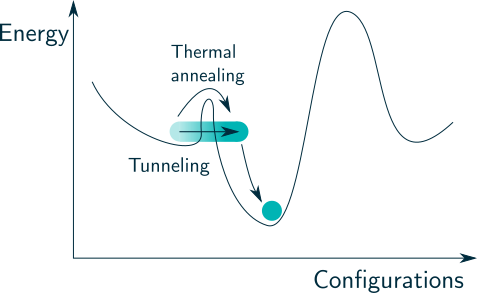
\includegraphics{figures/Tunneling.png}
    \caption{Caption}
    \label{fig:Tunnelling}
\end{figure}

\begin{tcolorbox}[standard jigsaw,
    opacityback=0,  % this works only in combination with the key "standard jigsaw"
    boxrule=0.5pt,label={example1}]
    {\bf Example 1}
    \tcbline
Solve the light configuration problem with two lights involved. The bias are set to be -1 for both lights and the weight assigned between them is 2 \\
i.e. Get the configuration to minimize the quadratic polynomial $-x_0-x_1+2x_0x_1$  
\end{tcolorbox}
\begin{lstlisting}[language=python]
from qdk import* 
# Create a quadratic polynmial  -x_0-x_1+2x_0x_1  
builder = QuadraticBinaryPolynomialBuilder() 
builder.add_term(-1.0, 0, 0) 
builder.add_term(-1.0, 1, 1) 
builder.add_term(2.0, 1, 0)  
quad_poly = builder.build_polynomial() 
# Create a local solver  
dwave_local_solver = DWaveSolver() 
# Get configuration of minimum energy solution 
solution_list = dwave_local_solver.minimize(quad_poly) 
print solution_list.solution_count 
sol=solution_list.peek_minimum_energy_solution() 
print sol 
\end{lstlisting}

Vertex coloring problem is probably one of the most popular NP problems. Given the graph G(V, E) with the set of vertices V and the set of edges E, it is to determine the coloring configuration of the vertices for which no adjacent two nodes (the nodes connected with edge) have the same color. \\ 
Mathematically it is the same as finding the minimum value for:
\begin{equation}
H = \sum_{n=0}^{N-1}(1-\sum_{k=0}^{K-1}x_{n,k})^2 + \sum_{(u,v)\in E}\sum_{k=0}^{K-1}x_{u,k}x_{v,k}
\end{equation}
$x_{n,k}$ with node n and color k is 1 only if the node n has color k, 0 otherwise. N is the total number of nodes and K is total number of the color used. The first term is the restriction that each node can only have one color. The second term is the restriction that the adjacent nodes have different color.  As only one dimensional QUBO problem can be solved, the equation (2) should be reduced to one dimension by reordering the index $n,k \rightarrow nK+k$. 
\begin{tcolorbox}[standard jigsaw,
    opacityback=0,  % this works only in combination with the key "standard jigsaw"
    boxrule=0.5pt,label={example1}]
    {\bf Example 2}
    \tcbline 
  Vertex  coloring problem for configuration showed in (a)
    \end{tcolorbox}
   
\begin{lstlisting}[language=python, caption={code adapted from KColoring.ipynb on   \url{ http://qdk.1qbit.com/}   }, label={code}]
import networkx as nx 
import matplotlib.pyplot as plt 
# Set the graph configuration by setting nodes and neighbours 
node=[0,1,2,3,4] 
neighbour=[(0,4),(1,2),(1,3),(1,4)] 
# Draw the graph configuration 
g=nx.Graph() 
g.add_nodes_from(node) 
g.add_edges_from(neighbour) 
pos = nx.spring_layout(g) 
nx.draw(g, pos=pos, with_labels=True) 
plt.show() 
# Turn the two dimension index to one dimension
def ind2to1(i, j, r):  
 return i * r + j  
pallete = {0: 'r', 1: 'c', 2:'m', 3:'y'} 
def get_color(i, sol, r): 
 z = ind2to1(i, 0, r) 
 ctr = 0 
 for ctr in range(r): 
  if sol[z + ctr]: 
   break 
 return pallete[ctr] 
# Construct the quadratic equation (3.2) with one dimension index
from qdk.binary_polynomial import * 
from qdk.common_solver_interface import * 
builder = QuadraticBinaryPolynomialBuilder() 
qubo = builder.build_polynomial() 
N = 5 
K = 4
for n in range(N): 
 builder.add_constant_term(1) 
for k in range(K): 
 builder.add_term(-1, ind2to1(n,k,K)) 
l=builder.build_polynomial() 
builder.power(2) 
t = builder.build_polynomial() 
qubo.sum(t) 
builder.reset() 
for (u,v) in g.edges(): 
 for k in range(K):  
  builder.add_term(1, ind2to1(u,k,K), ind2to1(v,k,K)) 
qubo.sum(builder.build_polynomial()) 
print qubo 
# Get the minimum energy solution by taking 300 samples
solver = DWaveSolver() 
solver.solver.num_reads = 300 
sol = solver.minimize(qubo).peek_minimum_energy_solution().configuration 
print sol 
# Draw the final configuration with color applied
nx.draw(g, pos=pos, with_labels=True, nodelist=g.nodes(),  
node_color=[get_color(i, sol, K) for i in g.nodes()]) 
plt.show() 
\end{lstlisting}
\begin{figure}
    \centering
    \begin{subfigure}[b]{0.4\textwidth}
        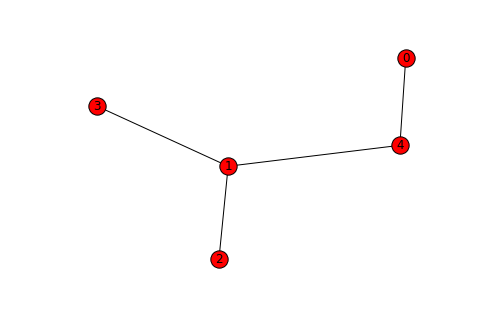
\includegraphics[width=\textwidth]{graph.png}
        \caption{A gull}
        \label{fig:gull}
    \end{subfigure}
     \begin{subfigure}[b]{0.4\textwidth}
        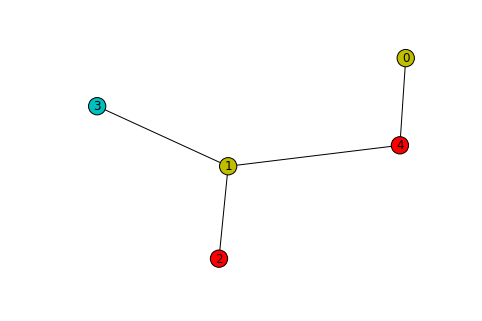
\includegraphics[width=\textwidth]{figures/colored.png}
        \caption{A gull coloured}
        \label{fig:gull}
    \end{subfigure}
\end{figure}[]



%%%%%%%%%%%%%%%%

\newpage
%\begin{multicols}{2}


%%%%%%%%%%%%%%%%%%%%%%%%%%%%%%%%%%%%%%%
\section{Implementing an Eigensolver's algorithm}
%%%%%%%%%%%%%%%%%%%%%%%%%%%%%%%%%%%%%%%


%%%%%%%%%%%%%%%%%%%%%%%%%%%%%%%%%%%%%%%%%%%
\subsection{Eigensolver's Algorithm with pyQuil}
%%%%%%%%%%%%%%%%%%%%%%%%%%%%%%%%%%%%%%%%%%%

Loading...

\newpage
%%%%%%%%%%%%%%%%%%%%%%%%%%%%%
\subsection{Eigensolver Algorithm in QISKit}
%%%%%%%%%%%%%%%%%%%%%%%%%%%%%
Applications that can use the five-qubit register include simulation of quantum state evolution and computing the properties of a ground state of the system. These applications are useful for quantum chemistry and solid state physics, where understanding strongly-correlated fermions is of interest. QISKit ACQUA provides tools that can be used to make an eigensolver for the ground state energy of simple molecules. The ground state problem may be understood as finding the solution to $H\ket{\psi_{g}}=E_{g}\ket{\psi_{g}}$, where $H$ represents the Hamiltonian (energy operator) of the system and $\ket{g}$ and $E_{g}$ represent the ground state and its associated energy, respectively. For complex systems such as molecules, the ground state energy can be challenging to compute in a simplified way. We need ACQUA to run these sorts of simulations as its library has a number of tools that simplify the process.
QISKit ACQUA requires a number of external files to run its computation. It is recommended that these steps be taken in the route to simulating molecular ground state energies with ACQUA on QISKit. The other application is in simulating the ising model of spin chains, though we will not cover this in this section.
\begin{itemize}
    \item Download the latest version of Anaconda Navigator in Python 3.6 at: \url{https://www.anaconda.com/download/}
    \item Download the relevant QISKit files from the website: \url{https://nbviewer.jupyter.org/github/QISKit/qiskit-tutorial/blob/master/index.ipynb}
    \item Sign up for QISKit via IBM Q experience and generate an API key for your Qconfig.py file found in the downloads from the QISKit website 
    \item Use the command prompt to install with: pip install qiskit qiskit-acqua qiskit-acqua-chemistry in Anaconda
\end{itemize}
The molecule in this example will be Lithium hydride (LiH), as seen in \autoref{acqua}. The Hartree Fock method (used to determine the quantum state of a multi-particle system) is used to describe the initial state of the molecule. More detail on this method of state determination can be found in \cite{hartreefockmethod}.  
\begin{lstlisting}[language=Python,float=h!,caption={The Lithium hydride eigensolver with Hartree Fock initial state adapted from \url{https://qiskit.org/acqua/chemistry}.}, label=acqua]
from qiskit_acqua_chemistry import ACQUAChemistry
# Define the problem using the parameters in the acqua dictionary
acqua_chemistry_dict = {
'driver': {'name': 'PYSCF'}, # Psycf driver for writing molecular configuration and species
# Writes the positions of the atoms in the molecule in 3 dimensions
'PYSCF': {'atom': 'Li .0 .0 -0.8; H .0 .0 0.8', 'basis': 'sto3g'},  
# Maps Hamiltonian with parity qubit mapping and two-qubit reduction. Reduces the orbital size as well 
'operator': {'name':'hamiltonian','qubit_mapping': 'parity', 'two_qubit_reduction': True, 'freeze_core': True, 'orbital_reduction': [-3,-2]},
'algorithm': {'name':'VQE'}, # Variational quantum eigensolver
# Iterates the optimizer COBYLA 10000 times
'optimizer': {'name':'COBYLA','maxiter': 10000},
'variational_form': {'name':'UCCSD'}, 
# Hartree Fock initial state calculation
'initial_state': {'name': 'Hartree Fock'}, 
# Simulation performed on the local simulator
'backend':{'name': 'local_qasm_simulator'} 
}
solver = ACQUAChemistry()
result = solver.run(acqua_chemistry_dict)
print(result['energy']) # Prints the result of the calculation for the ground state energy
\end{lstlisting}
Constrained optimisation by linear approximation (COBYLA) is the numerical optimisation, among possible others, which is used in this example. The maximum number of iterations can be altered to suit the example along with the options to print convergence trends and termination tolerance. The backend can be changed to ibmqx4 for other examples by using an API token and experiment credits on IBM Q experience. You can compare results between the two backend options to see how well ibmqx4 compares to your classical simulation. (Another example could be added after this where there are additional elements to code by the user, perhaps an exercise on this would be helpful)
\newpage

%%%%%%%%%%%%%%%%%%%%%%%%%%%%%%%%%%%%%%%%%%%
\subsection{Eigensolver's Algorithm with Project Q?}
%%%%%%%%%%%%%%%%%%%%%%%%%%%%%%%%%%%%%%%%%%%


%%%%%%%%%%%%% Old Deusch algm
\begin{comment}
\begin{multicols}{2}
%%%%%%%%%%%%%%%%%%%%%%%%%%%%%%%%


%%%%%%%%%%%%%%%%%%%%%%%%%%%%%%%%
\subsection{Deutsch's Algorithm}
%%%%%%%%%%%%%%%%%%%%%%%%%%%%%%%%

%%%%%%%%%%%%%%%%
\begin{tcolorbox}[standard jigsaw,
    opacityback=0,  % this works only in combination with the key "standard jigsaw"
    boxrule=0.5pt]
    {\bf Deutsch's Algorithm}
    \tcbline
    Given a function $f:\{0,1\}^2\rightarrow \{0,1\}$ promised to be either balanced or constant. We initialise the system in the state $\ket{00}$, we need to implement the gates $H^{\otimes 2}$ and then $U_f$ and then $H^{\otimes 2}$ and then perform a measurement in the computational basis.
\end{tcolorbox}
%%%%%%%%%%%%%%%

%%%%%%%%%%%%%%%%%
\begin{lstlisting}[language=Python,caption={Deutsch's algorithm implemented in Python only},label={lst:DApython},frame=single] 
import numpy as np
# State initialisation
state0=np.array([[1],[0],[0],[0]]) 
# Gate Implementation
H=(1/np.sqrt(2))*np.array([[1,1],[1,-1]]) 
state1=np.dot(np.kron(H,H),state0)        
U=np.array([[-1,0,0,0],
            [0,1,0,0],
            [0,0,-1,0],
            [0,0,0,1]])
state2=np.dot(U,state1)
state3=np.dot(np.kron(H,H),state2)
# Measurement: defining basis
ket0=np.array([[1],[0]])
ket1=np.array([[0],[1]])
ket00=np.kron(ket0,ket0)
ket01=np.kron(ket0,ket1)
ket10=np.kron(ket1,ket0)
ket11=np.kron(ket1,ket1)
# Measurement: projectors P00,P01,P10,P11
P00=np.dot(ket00,ket00.T)
P01=np.dot(ket01,ket01.T)
P10=np.dot(ket10,ket10.T)
P11=np.dot(ket11,ket11.T)
# Probability of obtaining: 00,01,10,11
prob00=np.trace(np.dot(P00,np.dot(state3,np.conj(state3).T)))
prob01=np.trace(np.dot(P01,np.dot(state3,np.conj(state3).T)))
prob10=np.trace(np.dot(P10,np.dot(state3,np.conj(state3).T)))
prob11=np.trace(np.dot(P11,np.dot(state3,np.conj(state3).T)))
print(prob00,prob01,prob10,prob11)
\end{lstlisting}
%%%%%%%%%%%%%%%%
\columnbreak

Now implementing this with pyQuil. We first need to learn how to add our own gates.

%%%%%%%%%%%%%%%%%
\begin{lstlisting}[language=Python]
# Defining our own gates
Ufma=np.array([[-1,0,0,0],
               [0,1,0,0],
               [0,0,-1,0],
               [0,0,0,1]]); 
p.defgate("Uf",Ufma); 
p.inst(("Uf",0,1)); 
\end{lstlisting}
%%%%%%%%%%%%%%%%

In \autoref{lst:DAqvm}

%%%%%%%%%%%%%%%%%
\begin{lstlisting}[language=Python,caption={Deutsch's algorithm with pyQuil},label={lst:DAqvm},frame=single]
import numpy as np
from pyquil.quil import Program
from pyquil.api import QVMConnection 
from pyquil.gates import X,Z,Y,H,I 
# Invoking and renaming
qvm=QVMConnection()
p=Program() 
# Gate implementation
p.inst(H(0),H(1)) 
# Assuming the given function gives
Ufma=np.array([[-1,0,0,0],
               [0,1,0,0],
               [0,0,-1,0],
               [0,0,0,1]]);
# Adding matrix as a gate               
p.defgate("Uf",Ufma); 
# Applying new gate and Hadamards
p.inst(("Uf",0,1)); 
p.inst(H(0),H(1))
# Measurements
p.measure(0,0)
p.measure(1,1) 
# Running the program
cr=[] 
results=qvm.run(p,cr,4) 
print(results)
\end{lstlisting}
%%%%%%%%%%%%%%%%

%%%%%%%%%%%%%%%%
\begin{tcolorbox}[standard jigsaw,
    opacityback=0,  % this works only in combination with the key "standard jigsaw"
    boxrule=0.5pt]
    {\bf Exercise 2: Bernstein-Vazirani Algorithm}
    \tcbline
    As in DJ with $n=3$, and given a function $f$ that is a parity function. Checking that the code indeed identifies the parity function
\end{tcolorbox}

\end{multicols}
\end{comment}
%%%%%%%%%%%%%


%%%%%%%%%%%%%% Old Rigetti code added by Ben
\begin{comment}
Rigetti has created an environment called Forest, amongst its contributions is a python library called PyQuil. With PyQuil one can simulate up to 26 qubits on the Quantum Virtual Machine (QVM). An example code from \cite{rigetti} is detailed below with comments to assist the reader:
%%%%%%%%%%%%%%%%%%%%%%%%%%%%%%%%%%%
\begin{lstlisting}[language=Python,float=h]
from pyquil.quil import Program
from pyquil.gates import H, CNOT
from pyquil.api import SyncConnection
# construct a Bell State program
p = Program()
p.inst(H(0))
p.inst(CNOT(0, 1))
# run the program on a QVM
qvm = SyncConnection()
result = qvm.wavefunction(p) 
# produces the output wavefunction of the Bell state
\end{lstlisting}
Rigetti also offers access to a 19 qubit processor they call 19Q. This API 
%%%%%%%%%%%%%%%%%%%%%%%%%%%%%%%%%%%%%%%%%%%
\begin{lstlisting}[language=Python,float=h]
import numpy as np
 
def incmatrix(genl1,genl2):
    m = len(genl1)
    n = len(genl2)
    M = None #to become the incidence matrix
    VT = np.zeros((n*m,1), int)  #dummy variable
 
    #compute the bitwise xor matrix
    M1 = bitxormatrix(genl1)
    M2 = np.triu(bitxormatrix(genl2),1) 
 
    for i in range(m-1):
        for j in range(i+1, m):
            [r,c] = np.where(M2 == M1[i,j])
            for k in range(len(r)):
                VT[(i)*n + r[k]] = 1;
                VT[(i)*n + c[k]] = 1;
                VT[(j)*n + r[k]] = 1;
                VT[(j)*n + c[k]] = 1;
 
                if M is None:
                    M = np.copy(VT)
                else:
                    M = np.concatenate((M, VT), 1)
 
                VT = np.zeros((n*m,1), int)
 
    return M
\end{lstlisting}
\end{comment}
%%%%%%%%%%%%%

%%%%%%%%%%%%%%%%%%%%%%%%%%%%%%%%%%%%%%%%
\chapter{Quantum Algorithms and Applications}
\label{Algorithmsandapplications}

\epigraph{You are not expected to understand this}{\textit{John Lions, Lions' Commentary on UNIX 6th Edition, with Source Code}}

In this section we discuss three of the most famous algorithms that provide some speed-up on a quantum computer for different problems. We start with two oracular algorithms, Deutsh's and Grover's. The last of these we go into in detail, as it is a useful example for developing some intuition of how superpositions can be used effectively. The other algorithms are described more briefly, as we outline some idea of how they work and provide a resource-focused outlook of the algorithm. Finally, several algorithms, their resource requirements and success probabilities are summed up in a table in section \ref{AlgorithmTable} for reference. 

\section{Oracular Algorithms}

Oracular algorithms are those which are based on a unitary operation called oracle. Suppose there is a function $f(x)$ on one-bit domain range, then there exits an operation which transforms the state $\ket{x,y} \rightarrow \ket{x,y \, \bigoplus f(x)}$, where $\bigoplus$ indicates addition modulo 2. It is well known that this operation is unitary and can be simulated by appropriate sequence of gates. More importantly, if this operation is applied to the state $\ket{x}(\ket{0}-\ket{1})/\sqrt{2}$, then it outputs the state $(-1)^{f(x)}\ket{x}(\ket{0}-\ket{1})/\sqrt{2}$. This operation is generally known as oracle and represented by $U_{f}$. There are many algorithms which exploit this operation because it allows to do computation by phase manipulation. Some of the well known algorithms have been discussed below.

%%%%%%%%%%%%%%%%%%%%%%%%%%%%%%%%
%%%%%%%%%%%%%%%%%%%%%%%%%%%%%%%%
\subsection{Deutsch-Jozsa algorithm}
%%%%%%%%%%%%%%%%%%%%%%%%%%%%%%%%
%%%%%%%%%%%%%%%%%%%%%%%%%%%%%%%%

Deutsch-Jozsa algorithm is one of the first algorithms to demonstrate ``quantum parallelism''. In very simple terms, quantum parallelism is a feature of quantum computer which allows it to evaluate a function $f(x)$ simultaneously for many different values of $x$. Deutsch-Jozsa algorithm doesn't have many practical applications but it does provide insight into how quantum computing can trump classical computation. Suppose there is a function $f(x): \{0,1\}^{n} \rightarrow \{0,1\}$ which is either constant or balanced for all values of $x$, the problem is to find with certainty the nature of $f(x)$. A classical solver would need at least $N=2^{n}/2+1$ queries to determine with certainty whether the function is balanced or constant while the quantum algorithm can solve the problem in just one query. The box below describes how Deutsch-Jozsa algorithm features the property of quantum parallelism for a 2-qubit case $(N=2^{2}=4)$. It should be noted that there is an additional qubit required for oracle as well.

\begin{tcolorbox}[standard jigsaw,
    opacityback=0,  % this works only in combination with the key "standard jigsaw"
    boxrule=0.5pt,label={Deutsch's algorithm box}]
    {\bf Deutsch-Jozsa Algorithm}
    \tcbline
    \begin{enumerate}
    \item Start with the state $\ket{00}$.
    \item Apply Hadamard gate to all the qubits which leads to the state: $\ket{\Psi}=\dfrac{1}{2}\big(\ket{0}+\ket{1}\big)\big(\ket{0}+\ket{1}\big)$.
    \item Apply the oracle `$U_{f}$' which transforms the state $\ket{\Psi} \rightarrow \dfrac{1}{2}\big((-1)^{f(00)}\ket{00}+(-1)^{f(01)}\ket{01}+(-1)^{f(10)}\ket{10}+(-1)^{f(11)}\ket{11}\big)$.
    \item Apply Hadamard to the first two qubits. Now, if $f(x)$ is constant, the first two qubits end up in the state $\ket{00}$ but if $f(x)$ is balanced, the first two qubits are in the state $\ket{01}$, $\ket{10}$ or $\ket{11}$.
    \item Measuring the first two qubits reveals the nature of $f(x)$.
    \end{enumerate}
\end{tcolorbox}

The circuit diagram for Deutsch-Jozsa algorithm for a general n-qubit case looks like:

\begin{equation*}
\Qcircuit @C=2.14em @R=1.25em
{\lstick{\ket{0}} & \gate{H} & \multigate{5}{U_f} & \gate{H} & \meter \\
\lstick{\ket{0}} & \gate{H} & \ghost{U_f} & \gate{H} & \meter \\ 
& \dot{} & & \dot{} \\
& \dot{} & & \dot{} \\
& \dot{} & & \dot{} \\
\lstick{\ket{0}} & \gate{H} & \ghost{U_f} & \gate{H} & \meter \\}
\end{equation*}

%%%%%%%%%%%%%%%%%%%%%%%%%%%%%%%
%%%%%%%%%%%%%%%%%%%%%%%%%%%%%%%
\subsection{Grover's algorithm}
%%%%%%%%%%%%%%%%%%%%%%%%%%%%%%%
%%%%%%%%%%%%%%%%%%%%%%%%%%%%%%%

One of the earliest algorithms that were designed to use quantum resources was described in 1996 paper by Lov Grover \cite{grover1996}. The algorithm attempts to solve the following problem: imagine you have a database of elements. We can represent them as bit strings, but we know that one of them is `marked' by some function acting on that bit string. Examining the case where we have 4 numbers (2 bits), we have the following truth table. 

\begin{equation}
\begin{array}{c|c|c}
    & x & f(x) \\
    \hline
    0 & 00 & 0 \\
    1 & 01 & 0 \\
    2 & 10 & 1 \\
    3 & 11 & 0 \\
\end{array}
\end{equation}

This unstructured search is an important problem in computer science. If we used a classical computer to try to find the marked element 10 above we'd have to try at least 3 times, since we could always end up with it being the last element applied to f(x). This scales as expected, so we can write that at worst it takes N attempts to find the marked element, which can be written O(N).

However, using the principle of superposition, we can explore the whole space of elements simultaneously. To do this we need two matrices (or gates): one which is a diagonal matrix with $(-1)^{f(x)}$ as its elements. For the marked element being 10 as above, we have

\begin{align}
        U_f = \begin{pmatrix}
        1 & 0 & 0 & 0 \\
                 0 & 1 & 0 & 0\\
                 0  & 0 & -1 & 0 \\
                 0 & 0 & 0 & 1
        \end{pmatrix}
\end{align}

The second ingredient is the following matrix, (irrespective of which element is marked)

\begin{align}
        D = \frac{1}{2}\begin{pmatrix}
        -1 & 1 & 1 & 1 \\
                 1 & -1 & 1 & 1\\
                 1  & 1 & -1 & 1 \\
                 1 & 1 & 1 & -1
        \end{pmatrix}
\end{align}

Now we will look at the algorithm step-by-step for this simple four element (two qubit) case. Starting with the qubits in the 00 state, we generate a superposition using a so called Hadamard gate (represented by H) on each qubit, which takes $00 \rightarrow 00 + 01 + 10 +11$ (we have ignored normalisation for simplicity). This can be represented by the matrix transformation

\begin{align}
        \frac{1}{2}
        \begin{pmatrix}
        1 & 1 & 1 & 1 \\
        1 & -1 & 1 & -1\\
        1  & 1 & -1 & -1 \\
        1 & -1 & -1 & 1
        \end{pmatrix}
        \begin{pmatrix}
        1\\
        0\\
        0\\
        0\\
        \end{pmatrix}
        =
        \frac{1}{2}
        \begin{pmatrix}
        1\\
        1\\
        1\\
        1\\
        \end{pmatrix}
\end{align}

In the next step of the algorithm, we apply $U_f$. This picks out the marked element, giving it a minus sign and adding a $\pi$ phase shift to the other elements.

\begin{align}
        \frac{1}{2}
        \begin{pmatrix}
        1 & 0 & 0 & 0 \\
        0 & 1 & 0 & 0\\
        0  & 0 & -1 & 0 \\
        0 & 0 & 0 & 1
        \end{pmatrix}
        \begin{pmatrix}
        1\\
        1\\
        1\\
        1\\
        \end{pmatrix}
        =
        \frac{1}{2}
        \begin{pmatrix}
        1\\
        1\\
        -1\\
        1\\
        \end{pmatrix}
\end{align}

The final step is to apply $D$. The construction is $D$ is such that each row, when multiplied by the vector, converts the $\pi$ phase difference into unit value . This can be thought of as a constructive interference on the marked element instead of destructive interference on all of the other elements. 

\begin{align}
    \frac{1}{2}.\frac{1}{2}
    \begin{pmatrix}
    -1 & 1 & 1 & 1\\
    1 & -1 & 1 & 1 \\
    1 & 1 & -1 & 1 \\
    1 & -1 & -1 & 1 \\
    \end{pmatrix}
    \begin{pmatrix}
    1 \\ 1 \\ -1 \\ 1 
    \end{pmatrix}
    =
    \frac{1}{4}
    \begin{pmatrix}
    0 \\ 0 \\ 4 \\ 0
    \end{pmatrix}
    = 
    \begin{pmatrix}
    0 \\ 0 \\ 1 \\ 0
    \end{pmatrix}
\end{align}

From this we can see that the general recipe of Grover's algorithm is to create a superposition of all the possible states, add a $\pi$ phase shift to the marked states with the special unitary $U_f$, and then use $D$ to pick out this phase shift.

In this case the algorithm has successfully found the marked element with certainty (though this does not take into account any experimental imperfections observed in real life). However, using superpositions inevitably leads to success with a non-unity success rate, as demonstrated in the next section, where we take the three qubit case. Furthermore we now look at using Dirac notation instead of matrices, as now we would have to use $8\times8$ matrices - this demonstrates the exponential scaling that quantum computing demonstrates, with $2^n\times2^n$ matrices being required for $n$ qubits. Hence the transition to Dirac notation is quite a natural progression to larger system sizes. 

%%%%%%%%%%%%%%%%%%%%%%%%%%%%%%%%%%%%%%%%%
\subsubsection{Alternative representation: Dirac notation}
We again consider a problem on $N=8$ elements, where the fifth element is marked. The algorithm can be applied with a minimum of $3$  ($2^{3}=8$) qubits in the following manner:

\begin{tcolorbox}[standard jigsaw,
    opacityback=0,  % this works only in combination with the key "standard jigsaw"
    boxrule=0.5pt,label={example1}]
    {\bf Grover's Algorithm}
    \tcbline
    \begin{enumerate}
    \item Start with the state $\ket{000}$.
    \item Apply the Hadamard gates which result in the state: $\ket{\Psi}=\dfrac{1}{2\sqrt{2}}\big(\ket{000}+\ket{001}+\ket{010}+\ket{011}+\ket{100}+\ket{101}+\ket{110}+\ket{111}\big)$
    \item Apply $U_{f}$, which reverses the sign on the fifth element: $\ket{\Psi}=\dfrac{1}{2\sqrt{2}}\big(\ket{000}+\ket{001}+\ket{010}+\ket{011}-\ket{100}+\ket{101}+\ket{110}+\ket{111}\big)$
    \item Apply D, which leads to state $\ket{\Psi}=\dfrac{1}{4\sqrt{2}}\big(\ket{000}+\ket{001}+\ket{010}+\ket{011}+5\ket{100}+\ket{101}+\ket{110}+\ket{111}\big)$
    \item Repeat steps 3 and 4 ``$T$'' times, where $T$ is to be determined later.
    \item Measure the state $\ket{\Psi}$.
    \end{enumerate}
\end{tcolorbox}



\begin{figure}
    \centering
    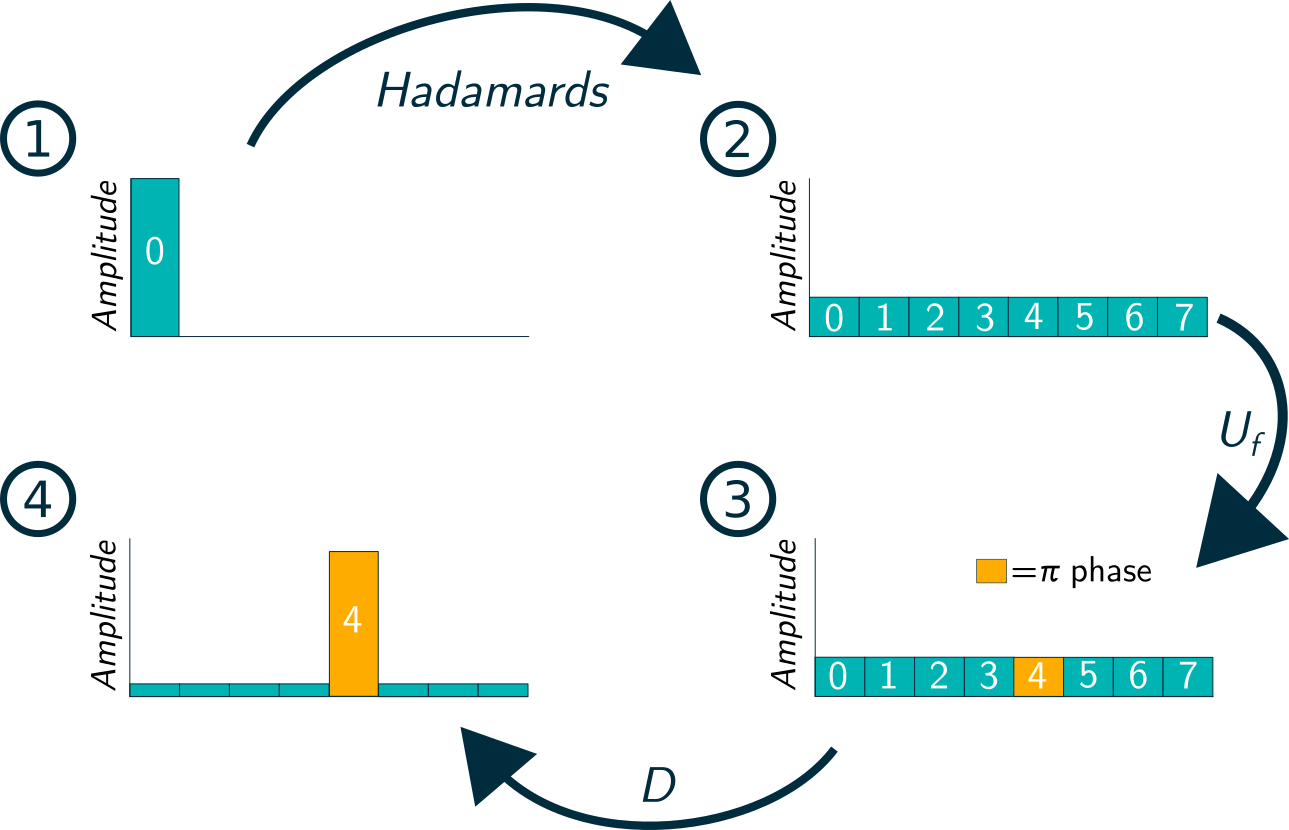
\includegraphics[width=0.9\linewidth]{figures/Grovers.png}
    \caption{Pictorial demonstration of the steps of Grover's Algorithm}
    \label{fig:Grovers}
\end{figure}


In the step 2 above, applying Hadamard gate to all the qubits leads to a state which is in superposition of all possible states (elements). It is important to start with the state $\ket{000}$ so that all the states in the superposition have the same initial phase. In step 3 we apply $U_{f}$ gate which is dependent on $f(x)$ and is able to recognise the marked element. What it does is that it applies a $\pi$ phase shift to the marked element but leaves all the other states unchanged. Next step is to apply gate $D$ to the state obtained in step 3. The application of gate $D$ can be understood as the operation which increases the amplitude of the phase shifted element in step 3. As mentioned in chapter 1, the measurement of a state leads to an output with a probability equal to the amplitude squared and thus, increasing the amplitude of the marked element state results in a higher probability of measuring that state. It is worth noting that repeating steps 3 and 4 a fixed number of times will increase the probability of detecting the marked element but after a certain point, the probability will start to decrease. For clarification, if we another iteration of step 3 and 4 in the above example, we get the state:
\begin{align}
\ket{\Psi}=\dfrac{-1}{8\sqrt{2}}\big(\ket{000}+\ket{001}+\ket{010}+\ket{011}-11\ket{100}+\ket{101}+\ket{110}+\ket{111}\big).
\end{align}
 Now if a measurement is performed on this state, there is a 94.53\% chance of getting the fifth element compared to 78.12\% probability if the measurement is performed after just one iteration. On the other side, if another iteration of step 3 and 4 is performed, the resulting state becomes:

\begin{align}
\ket{\Psi}=\dfrac{-7}{16\sqrt{2}}\big(\ket{000}+\ket{001}+\ket{010}+\ket{011}-\frac{13}{7}\ket{100}+\ket{101}+\ket{110}+\ket{111}\big)    
\end{align}
and the probability of getting the marked element upon measurement is only 67\% in this case. Therefore, it is important to choose the number of iterations for Grover's algorithm very carefully. The number of iterations ``$T$'' required to get the maximum probability of measuring the marked element is approximated as $T=\big(\pi\big/4)\sqrt{N}$.

%%%%%%%%%%%%%%%%%%%%%%%%%%%%%%%%%%%%
\subsubsection{General n-qubit case}

Given a function $f: \left\{0,1\right\}^n \rightarrow \left\{0,1\right\}$ with the promise that $f(x_0) = 1$ for a unique element $x_0$, the problem is to find this $x_0$. We use a quantum circuit on $n$ qubits with initial state $\ket{0}^{\otimes n}$.  Let $H$ denote the Hadamard gate, and let $U_0$ denote the $n$-qubit operation which inverts the phase of $\ket{0^n}$: $U_0\ket{0^n} = -\ket{0^n}$, $U_0\ket{x} = \ket{x}$ for all $x \neq 0^n$. The first step of the algorithm is to apply Hadamard gate on all $n$ qubits. Next, repeat the following operations T times for some T to be determined later.
%\begin{enumerate}
%\item Apply $H^{\otimes n}$.

%\item Repeat the following operations T times, for some T to be determined later:
\begin{enumerate}
\item Apply $U_f$, where $U_f\ket{x} = (-1)^{f(x)}\ket{x}$.
\item Apply $D$, where $D = -H^{\otimes n}U_0H^{\otimes n}$
\end{enumerate} 
%\item Measure all the qubits and output the result.
%\end{enumerate}
%\end{tcolorbox}
Finally, measure all the qubits and output the result.\\

In circuit diagram form, Grover's algorithm appears like: \\
\begin{equation*}
\Qcircuit @C=2.14em @R=1.25em
{\lstick{\ket{0}} & \gate{H} & \multigate{5}{U_f} & \multigate{5}{D} & \multigate{5}{U_f} & \ghost{U_f} & \lstick{\dots} & \multigate{5}{D} & \meter \\
\lstick{\ket{0}} & \gate{H} & \ghost{U_f} & \ghost{D} & \ghost{U_f} & \ghost{U_f} &\lstick{\dots} & \ghost{D} & \meter \\ 
& \dot{} & & & & & & & \dot{} \\
& \dot{} & & & & & & & \dot{} \\
& \dot{} & & & & & & & \dot{} \\
\lstick{\ket{0}} & \gate{H} & \ghost{U_f} & \ghost{D} & \ghost{U_f} & \ghost{U_f} & \lstick{\dots} & \ghost{D} & \meter \\}
\end{equation*}

\subsubsection{Construction of gate $D$ and $U_{f}$}
The gate $D$ in the algorithm applied on $n$-qubits can be implemented in the following manner. This shows that gate $D$ requires $2n+1$ Hadamard ($H$) gates, $2n+1$ Pauli $X$ gates and an n-control Toffoli gate.

\begin{align*}
\Qcircuit @C=1.14em @R=1.25em
{\lstick{\ket{x_1}} & \gate{H} & \gate{X} &  \ctrl{1} & \gate{X} & \gate{H} & \qw  \\
\lstick{\ket{x_2}} & \gate{H} & \gate{X} &  \ctrl{4} & \gate{X} & \gate{H} & \qw  \\
\lstick{\dot{}} & \dot{} & \dot{} & & \dot{} & \dot{} & \\
\lstick{\dot{}} & \dot{} & \dot{} & & \dot{} & \dot{} & \\
\lstick{\dot{}} & \dot{} & \dot{} & & \dot{} & \dot{} & \\
\lstick{\ket{x_n}} & \gate{H} & \gate{X} &  \ctrl{1} & \gate{X} & \gate{H} & \qw  \\
\lstick{\ket{0}} & \gate{x} & \gate{H} &  \targ & \qw & \qw & \qw }
\end{align*}

\vspace{1cm}
The construction of gate $U_{f}$ depends upon the function $f(x)$ being addressed by the algorithm.

%%%%%%%%%%%%%%%%%%%%%%%%%%%%
%%%%%%%%%%%%%%%%%%%%%%%%%%%%
%%%%%%%%%%%%%%%%%%%%%%%%%%%%
%%%%%%%%%%%%%%%%%%%%%%%%%%%%
\section{Quantum fourier transform}

Quantum Fourier transform (QFT) is the quantum analogue of discrete Fourier transform. It thus converts periodic functions to their conjugate domain (for example, time $\rightarrow$ frequency, position $\rightarrow$ momentum etc). Crucially it acts on quantum states. For example the QFT acting on two qubits is given by the transformation matrix 

\begin{align}
    QFT = 
    \frac{1}{2}
    \begin{pmatrix}
        \omega_N^{0} & \omega_N^{0} & \omega_N^0 &\omega_N^0 \\
        \omega_N^0 & \omega_N^1 & \omega_N^2 & \omega_N^3 \\
        \omega_N^0 & \omega_N^2 & \omega_N^4 & \omega_N^6 \\
        \omega_N^0 & \omega_N^3 & \omega_N^6 & \omega_N^9 \\
    \end{pmatrix}
    =
    \frac{1}{2}
    \begin{pmatrix}
        1 & 1 & 1 & 1 \\
        1 & i & -1 & -i \\
        1 & -1 & 1 & -1 \\
        1 & i & -1 & i \\
    \end{pmatrix}
\end{align}

This can be generalised to $n$ qubits, which requires a $2^n$ dimensional matrix with its elements given by 

\begin{align}
    QFT_{jk} = \omega_N^{jk} = \exp^{2\pi ijk / N} 
\end{align}

where we count the first columns and rows of the matrix from 0. The Quantum Fourier Transform can be constructed out of more fundamental quantum gates, a Hadamard gate and a controlled phase gate. 

 \begin{align}
    H = 
    \begin{pmatrix}
    1 & 1 \\
    1 & -1 \\
    \end{pmatrix},
    \quad
    R_n = 
    \begin{pmatrix}
    1 & 0\\
    0 & \omega_{2^n}\\
    \end{pmatrix}
 \end{align}
 
 This requires $n(n-1)/2$ controlled phase gates in total and $n$ Hadamard gates. 

The QFT is not an algorithm \textit{per se} but is crucial in many algorithms, such as Shor's algorithm as described in \ref{Shor's algorithm}.


%%%%%%%%%%%%%%%%%%%%%%%%%%%%%%%%%%

%%%%%%%%%%%%%%%%%%%%%%%%%%%%%
%%%%%%%%%%%%%%%%%%%%%%%%%%%%%
\section{Shor's algorithm}
%%%%%%%%%%%%%%%%%%%%%%%%%%%%%
%%%%%%%%%%%%%%%%%%%%%%%%%%%%%

\label{Shor's algorithm}

Shor's algorithm is a procedure to factor a large number. However, most of the steps in Shor's algorithm are in fact classical, and phrase the problem to be solved as one of finding the periodicity of a function. It uses a result from Euler that states that the The algorithm is given in box 

\begin{tcolorbox}[standard jigsaw,
    opacityback=0,  % this works only in combination with the key "standard jigsaw"
    boxrule=0.5pt,label={Shor's algorithm box}]
    {\bf Shor's algorithm}
    \tcbline
    \begin{enumerate}
    \item Pick a number $a<N$
    \item Calculate the greatest common divisor of this number $a$ and $N$, gcd($a,N$). If we obtain a number other than 1, then we have found a factor of $N$, so output gcd$(a,n)$ as our factor for $N$.
    \item Otherwise, find the period of the function $f(x) = a^x \mod N$. Label this period $r$
    \item Since  $a^0 \mod N = a^r \mod N = 1$, then $a^r - 1 \mod N = 0$. Factoring, $a^r-1 \mod N = (a^{r/2} - 1)(a^{r/2} + 1) \mod N = 0$. Thus $(a^{r/2} - 1)(a^{r/2} + 1) = lN$ for some integer $l$. If we found $r$ to be odd then this method has failed: return to 1. 
    \item Output either gcd($a^{r/2}-1$) or gcd($a^{r/2}+1$) as the factors of $N$.
    \end{enumerate}
\end{tcolorbox}

However, step 3 is not efficient classically. We can however use a quantum algorithm to provide a polynomial speed-up. We shall now explain to explain the machinery behind this process, attempting to develop an intuition for the quantum effects over the fine detail of this process. The diagram demonstrates the processes which occur. 


[DIAGRAM OF AMPLITUDES AND PHASES GO HERE, FOLLOWED BY EXPLANATION]



The circuit shown below implements Shor's algorithm. The $1^{st}$ register uses Hadamard gates to put the qubits in a uniform superposiiton. The second step uses an Oracle operation $U_f$ for a periodic function $f=a^x \mod N$ which has the following effect on the first and second registers:

\begin{align}
    U_f\ket{x}\ket{0} = \ket{x}\ket{f(x)}
    U_{a^x\mod N}\ket{x}\ket{0} = \ket{x}\ket{a^x\mod N}
\end{align}


measuring the second register then collapses it to a single $f_0 = f(x_0)$, where $f(x_0) = f(x_0 + r) = f(x_0 + 2r) = ...$ for the periodicity $r$ of the function. Thus the first register, through entanglement, is now in the a superposition of the states $\ket{x_0+jr}$ for all integers $j$ allowed for $x_0+jr$ to be within the register. Therefore we have a periodic superposition of a state, generating peaks in the spectrum as can be seen in [REF TO DIAGRAM TO BE ADDED]. This is a problem that can be clearly solved by the QFT - we have states that are periodic with period $r$ in one (Hilbert) space, and applying the inverse QFT will obtain a single strong peak at $r$.

\begin{figure}
\begin{align*}
\Qcircuit @C=2.14em @R=1.8em
{
& & & \lstick{\ket{0}} & \gate{H} & \multigate{7}{U_f} & \qw & \multigate{4}{QFT^{-1}} & \meter \\
& & &\lstick{\vdots} & \vdots &                         &              &         & \lstick{\vdots}  \\
& \push{\mathrm{1^{st}\,register}} & &\lstick{\ket{0}} & \gate{H} &           \ghost{U_f} & \qw &\ghost{QFT^{-1}} & \meter \\
&   &&\lstick{\ket{0}} & \gate{H} &           \ghost{U_f} & \qw &\ghost{QFT^{-1}} & \meter \\
&                   &&\lstick{\ket{0}} & \gate{H} &           \ghost{U_f} & \qw &\ghost{QFT^{-1}} & \meter \\
&                   &&\lstick{\ket{0}} & \qw &               \ghost{U_f} &  \meter \\
& \push{\mathrm{2^{nd}\,register}}              & &\lstick{\vdots} &       &                   &\lstick{\vdots} \\
&                   &&\lstick{\ket{0}} & \qw &       \ghost{U_f} & \meter  \gategroup{1}{3}{5}{3}{1.7em}{\{}
\gategroup{6}{3}{8}{3}{1.7em}{\{}}
\end{align*}
\caption{This circuit implements Shor's algorithm.}
\label{fig:apprPerAlgAlternative}
\end{figure}


\begin{sidewaystable}
\begin{tabular}{|c|c | c | c |c|}
    \hline
    \thead{Algorithm \\ name} & \thead{Purpose} & \thead{Number of \\qubits used} & \thead{Number of \\gates required} & \thead{Probability\\ of success}  \\
    
    \hline
    
    \makecell{Grover's \\algorithm} & \makecell{Unstructured \\search} & \makecell{$n$ qubits for \\$2^n$ marked \\elements} & \makecell{$(2T+1)n$ Hadamard gates,\\$T$ $U_f$ gates, and $T$ $U_0$ gates, \\where $T \approx \frac{\pi}{4} \sqrt{2^n}$} & $\sin^2((2T+1)\arcsin{\frac{1}{\sqrt{2^n}}})$\\
    \hline
    
    \makecell{Quantum period \\finding\\} & \makecell{Finding \\Periodicity} &  & & \\
    \hline
    
    \makecell{Deutsch-Jozsa\\algorithm\\} & \makecell{Constant or \\Balanced function} & \makecell{$n+1$ qubits for\\$2^n$ elements} & \makecell{One $U_{f}$ gate and\\$2n+1$ Hadamard gates}& \makecell{100\%}\\
    \hline
    
    \makecell{Eigensolver} & & & & \\
    \hline
    
    \end{tabular}
\end{sidewaystable}

%%%%%%%%%%%%%%%%%%%%%%%%%%%%%%%%%%%%%%%%%%%%%
\chapter{Programming a future universal quantum computer}
\label{Programmingquantumcomputer}

\epigraph{\textit{Don't believe everything you read on the Internet}}{Abraham Lincoln}

Three languages will be covered here: 
\begin{itemize}
    \item Quil
    \item QISKit 
    \item Q\#
    \item Project Q
\end{itemize}

Algorithms to implement:
\begin{itemize}
    \item Shor's algorithm (as example)
    \item Deutsch's algorithm (as exercise)
    \item Grover's algorithm (as exercise) (Ankur and David have already organised this one, so it'd be nice :3) 
    \item Deutsch's algorithm (as exercise/example)
\end{itemize}

\newpage
%%%%%%%%%%%%%%%%%%%%%%%%%%%%%%%%
%%%%%%%%%%%%%%%%%%%%%%%%%%%%%%%%
%%%%%%%%%%%%%%%%%%%%%%%%%%%%%%%%
%%%%%%%%%%%%%%%%%%%%%%%%%%%%%%%%
\section{Implementing Deutsch's Algorithm}
%%%%%%%%%%%%%%%%%%%%%%%%%%%%%%%%
%%%%%%%%%%%%%%%%%%%%%%%%%%%%%%%%
%%%%%%%%%%%%%%%%%%%%%%%%%%%%%%%%
%%%%%%%%%%%%%%%%%%%%%%%%%%%%%%%%

%%%%%%%%%%%%%%%%%%%%%%%%%%%%%%%%%%%%%%%%%%%
\subsection{Deutsch's Algorithm with pyQuil}
%%%%%%%%%%%%%%%%%%%%%%%%%%%%%%%%%%%%%%%%%%%

%%%%%%%%%%%%%%%%
\begin{tcolorbox}[standard jigsaw,
    opacityback=0,  % this works only in combination with the key "standard jigsaw"
    boxrule=0.5pt]
    {\bf Deutsch's Algorithm}
    \tcbline
    Given a function $f:\{0,1\}^2\rightarrow \{0,1\}$ promised to be either balanced or constant. We initialise the system in the state $\ket{00}$, we need to implement the gates $H^{\otimes 2}$ and then $U_f$ and then $H^{\otimes 2}$ and then perform a measurement in the computational basis.
\end{tcolorbox}
%%%%%%%%%%%%%%%

%%%%%%%%%%%%%%%%%
\begin{lstlisting}[language=Python,caption={Deutsch's algorithm implemented in Python only},label={lst:DApython},frame=single] 
import numpy as np
# State initialisation
state0=np.array([[1],[0],[0],[0]]) 
# Gate Implementation
H=(1/np.sqrt(2))*np.array([[1,1],[1,-1]]) 
state1=np.dot(np.kron(H,H),state0)        
U=np.array([[-1,0,0,0],
            [0,1,0,0],
            [0,0,-1,0],
            [0,0,0,1]])
state2=np.dot(U,state1)
state3=np.dot(np.kron(H,H),state2)
# Measurement: defining basis
ket0=np.array([[1],[0]])
ket1=np.array([[0],[1]])
ket00=np.kron(ket0,ket0)
ket01=np.kron(ket0,ket1)
ket10=np.kron(ket1,ket0)
ket11=np.kron(ket1,ket1)
# Measurement: projectors P00,P01,P10,P11
P00=np.dot(ket00,ket00.T)
P01=np.dot(ket01,ket01.T)
P10=np.dot(ket10,ket10.T)
P11=np.dot(ket11,ket11.T)
# Probability of obtaining: 00,01,10,11
prob00=np.trace(np.dot(P00,np.dot(state3,np.conj(state3).T)))
prob01=np.trace(np.dot(P01,np.dot(state3,np.conj(state3).T)))
prob10=np.trace(np.dot(P10,np.dot(state3,np.conj(state3).T)))
prob11=np.trace(np.dot(P11,np.dot(state3,np.conj(state3).T)))
print(prob00,prob01,prob10,prob11)
\end{lstlisting}
%%%%%%%%%%%%%%%%
%\columnbreak

Now implementing this with pyQuil. We first need to learn how to add our own gates.

%%%%%%%%%%%%%%%%%
\begin{lstlisting}[language=Python]
# Defining our own gates
Ufma=np.array([[-1,0,0,0],
               [0,1,0,0],
               [0,0,-1,0],
               [0,0,0,1]]); 
p.defgate("Uf",Ufma); 
p.inst(("Uf",0,1)); 
\end{lstlisting}
%%%%%%%%%%%%%%%%

In \autoref{lst:DAqvm}

%%%%%%%%%%%%%%%%%
\begin{lstlisting}[language=Python,caption={Deutsch's algorithm with pyQuil},label={lst:DAqvm},frame=single]
import numpy as np
from pyquil.quil import Program
from pyquil.api import QVMConnection 
from pyquil.gates import X,Z,Y,H,I 
# Invoking and renaming
qvm=QVMConnection()
p=Program() 
# Gate implementation
p.inst(H(0),H(1)) 
# Assuming the given function gives
Ufma=np.array([[-1,0,0,0],
               [0,1,0,0],
               [0,0,-1,0],
               [0,0,0,1]]);
# Adding matrix as a gate               
p.defgate("Uf",Ufma); 
# Applying new gate and Hadamards
p.inst(("Uf",0,1)); 
p.inst(H(0),H(1))
# Measurements
p.measure(0,0)
p.measure(1,1) 
# Running the program
cr=[] 
results=qvm.run(p,cr,4) 
print(results)
\end{lstlisting}
%%%%%%%%%%%%%%%%

\newpage
%%%%%%%%%%%%%%%%%%%%%%%%%%%%%%%%%%%%%%%%%%%%
\subsection{Deutsch's Algorithm in Qasm (IBM Q-experience)}
%%%%%%%%%%%%%%%%%%%%%%%%%%%%%%%%%%%%%%%%%%%%
The Deutsch-Jozsa algorithm can be coded on this language as well. We begin by setting the bits in the register 
\begin{lstlisting}[language=Python,float=h]


\end{lstlisting}

%%%%%%%%%%%%%%%%%%%%%%%%%%%%%%%%%%%%%%%%%%%
\subsection{Deutsch's Algorithm with Project Q}
%%%%%%%%%%%%%%%%%%%%%%%%%%%%%%%%%%%%%%%%%%%

%%%%%%%%%%%%%%%%%%%%%%%%%%%%%%%%%%%%%%%%%%%
\subsection{Deutsch's Algorithm with Q\#}
%%%%%%%%%%%%%%%%%%%%%%%%%%%%%%%%%%%%%%%%%%%


\newpage
%%%%%%%%%%%%%%%%%%%%%%%%%%%%%%%%%%%%%%%%%
\subsection{Deutsch's Algorithm Exercises}
%%%%%%%%%%%%%%%%%%%%%%%%%%%%%%%%%%%%%%%%%

Implement the following algorithms in the language of your choice.

%%%%%%%%%%%%%%%%
\begin{tcolorbox}[standard jigsaw,
    opacityback=0,  % this works only in combination with the key "standard jigsaw"
    boxrule=0.5pt]
    {\bf Exercise 2: Deutsch-Josza Algorithm}
    \tcbline
    As in Deutsch algorithm but with $n>2$.
\end{tcolorbox}

%%%%%%%%%%%%%%%%
\begin{tcolorbox}[standard jigsaw,
    opacityback=0,  % this works only in combination with the key "standard jigsaw"
    boxrule=0.5pt]
    {\bf Exercise 3: Bernstein-Vazirani Algorithm}
    \tcbline
    As in DJ with $n=3$, and given a function $f$ that is a parity function. Checking that the code indeed identifies the parity function
\end{tcolorbox}

\begin{comment}
\newpage
%%%%%%%%%%%%%%%%%%%%%%%%%%%%%%%%%%%%%%%
%%%%%%%%%%%%%%%%%%%%%%%%%%%%%%%%%%%%%%%
%%%%%%%%%%%%%%%%%%%%%%%%%%%%%%%%%%%%%%%
%%%%%%%%%%%%%%%%%%%%%%%%%%%%%%%%%%%%%%%
\section{Implementing Grover's algorithm}
%%%%%%%%%%%%%%%%%%%%%%%%%%%%%%%%%%%%%%%
%%%%%%%%%%%%%%%%%%%%%%%%%%%%%%%%%%%%%%%
%%%%%%%%%%%%%%%%%%%%%%%%%%%%%%%%%%%%%%%
%%%%%%%%%%%%%%%%%%%%%%%%%%%%%%%%%%%%%%%

Loading...

%%%%%%%%%%%%%%%%%%%%%%%%%%%%%%%%%%%%%%%%%%%
\subsection{Grover's Algorithm with pyQuil}
%%%%%%%%%%%%%%%%%%%%%%%%%%%%%%%%%%%%%%%%%%%

%%%%%%%%%%%%%%%%%%%%%%%%%%%%%%%%%%%%%%%%%%%
\subsection{Grover's Algorithm with QISKit}
%%%%%%%%%%%%%%%%%%%%%%%%%%%%%%%%%%%%%%%%%%%

%%%%%%%%%%%%%%%%%%%%%%%%%%%%%%%%%%%%%%%%%%%
\subsection{Grover's Algorithm with Project Q}
%%%%%%%%%%%%%%%%%%%%%%%%%%%%%%%%%%%%%%%%%%%

%%%%%%%%%%%%%%%%%%%%%%%%%%%%%%%%%%%%%%%%%%%
\subsection{Grover's Algorithm with Q\#}
%%%%%%%%%%%%%%%%%%%%%%%%%%%%%%%%%%%%%%%%%%%

%%%%%%%%%%%%%%%%%%%%%%%%%%%%%%%%%%%%%%%%%
\subsection{Grover's Algorithm Exercises}
%%%%%%%%%%%%%%%%%%%%%%%%%%%%%%%%%%%%%%%%%

\end{comment}

\newpage
%%%%%%%%%%%%%%%%%%%%%%%%%%%%%%%%%%%%%%%
%%%%%%%%%%%%%%%%%%%%%%%%%%%%%%%%%%%%%%%
%%%%%%%%%%%%%%%%%%%%%%%%%%%%%%%%%%%%%%%
%%%%%%%%%%%%%%%%%%%%%%%%%%%%%%%%%%%%%%%
\section{Implementing Shor's algorithm}
%%%%%%%%%%%%%%%%%%%%%%%%%%%%%%%%%%%%%%%
%%%%%%%%%%%%%%%%%%%%%%%%%%%%%%%%%%%%%%%
%%%%%%%%%%%%%%%%%%%%%%%%%%%%%%%%%%%%%%%
%%%%%%%%%%%%%%%%%%%%%%%%%%%%%%%%%%%%%%%

Shor's algorithm one of the most well-known quantum algorithms, due to it's implications for the safety of the commonly used RSA encryption scheme. It is also interesting, as it demonstrates the way classical and quantum computing can be used together. A large part of the algorithm is classical, but an essential part uses the quantum computer for significant speed up. The algorithm is discussed in more detail in section \ref{Shor's algorithm}.

This section will go into detail how the quantum parts of the algorithm are written in the different languages, with the full code being provided in the Appendix/Github.

%%%%%%%%%%%%%%%%%%%%%%%%%%%%%%%%%%%%%%%%%
\subsection{Shor's algorithm with pyQuil}

The first thing to do is import the libraries required, Python has libraries which help with calculating the greatest common divisors and the continued fraction expansion convergents. From pyQuil, we need to import the functions that allow us create and run the program as discussed in \autoref{Quantum Programs with pyQuil}. We can also take advantage of an implementation of the Quantum Fourier Transform (QFT) in Grove. 

\lstinputlisting[language=Python, firstline=1, lastline=7]{code/pyQuil/shor_pyquil_guide.py}

The first step is to randomly select an integer $1 < a < N$ and if the greatest common divisor of $a$ and $N$ is not $1$, then we have found a factor. Otherwise, we continue onto the quantum part of the algorithm to find the order of $f(x) = a^x \text{ mod } N$. First, the size of the registers need to be defined.

\lstinputlisting[language=Python, firstline=42, lastline=44]{code/pyQuil/shor_pyquil_guide.py}

Next we can set up the connection to the QVM and initialise the program structure. pyQuil only labels qubits in one large register and since it is more helpful for us to have two registers, we can specify which qubits we wish to use for each register.

\lstinputlisting[language=Python, firstline=46, lastline=52]{code/pyQuil/shor_pyquil_guide.py}

Applying the QFT to the first register is now simple.

\lstinputlisting[language=Python, firstline=54, lastline=55]{code/pyQuil/shor_pyquil_guide.py}

A more difficult task is creating the bit oracle $O_f\ket{x}\ket{y} = \ket{x}\ket{y \oplus f(x)}$. pyQuil does not have a function that allows you to construct arbitrary mathematical operations between registers, so the bit oracle must be constructed as a matrix. The function below constructs this matrix (need to explain in more detail the indexing and change oracle to SWAP gates since this code is currently not functioning!).

\lstinputlisting[language=Python, firstline=11, lastline=21]{code/pyQuil/shor_pyquil_guide.py}

A new gate using this unitary matrix can be defined using the function \texttt{defgate}, and applied to both registers.

\lstinputlisting[language=Python, firstline=57, lastline=60]{code/pyQuil/shor_pyquil_guide.py}

The next step in the algorithm calls for measuring the second register. pyQuil does not allow you to measure more than one qubit at a time, so the measurement is done inside a loop and a classical address to store the measurement result at must be specified. The code below measures qubit $i$ and stores it in classical address $i$.

\lstinputlisting[language=Python, firstline=62, lastline=64]{code/pyQuil/shor_pyquil_guide.py}

Once the QFT has been applied to the first register and that register measured, the program to find the approximate periodicity of $f(x)$ is complete and can now be run on the QVM. The classical addresses to store the results in and the number of trials must be specified.

\lstinputlisting[language=Python, firstline=73, lastline=75]{code/pyQuil/shor_pyquil_guide.py}

Converting the output $y$ of the approximate periodicity part of the algorithm from binary into an integer is done using the code below. It is important to keep in mind that qubit 0 gives the least significant bit.

\lstinputlisting[language=Python, firstline=77, lastline=80]{code/pyQuil/shor_pyquil_guide.py}

The next steps of the algorithm - determining the order $r$ from the output $y$ and testing for failure cases - is classical and does not need to be expanded upon here. The full code is located in the Appendix/Github.

%%%%%%%%%%%%%%%%%%%%%%%%%%%%%%%%%%%%%%%%%
\subsection{Shor's algorithm with QISKit}

Within the framework of the QISKit SDK, there are no built in functions to call from either QISKit or ACQUA libraries, thus the quantum Fourier transform and the bit-wise oracle operations must be programmed in as separate functions for calling into the main program.

This implementation of Shor's will be implemented using IBM's Q QASM 32-qubit simulator.

To begin, we start my importing all of the relevant packages for running the program. These are called from QISKit and generic Python libraries:

\lstinputlisting[language=Python, firstline=1, lastline=7]{code/QISKit/shor_qiskit.py}


%%%%%%%%%%%%%%%%%%%%%%%%%%%%%%%%%%%%%%%%%%
\subsection{Shor's algorithm with ProjectQ}

We can follow the same steps as for pyQuil and QISKit since all these languages are Python based. The code for the classical part of the algorithm stays the same and so does the size of the registers. This time the functions that need to be imported from ProjectQ are,

\lstinputlisting[language=Python, firstline=5, lastline=6]{code/ProjectQ/shor_projectq_guide.py}

Since ProjectQ is run on a local simulator, your computer, it is good practice to make sure that the number of qubits required for the computation can actually be simulated to avoid crashing the computer. Most modern computers have 8GB of RAM which is exactly enough memory for 29 qubits, but there are other processes being run on the computer so you would only be able to simulate 28.

\lstinputlisting[language=Python, firstline=31, lastline=34]{code/ProjectQ/shor_projectq_guide.py}

Now we can load the simulator by calling \texttt{MainEngine} and allocate the two registers.

\lstinputlisting[language=Python, firstline=36, lastline=39]{code/ProjectQ/shor_projectq_guide.py}

The QFT is a standard operation in ProjectQ and the syntax for applying it is,

\lstinputlisting[language=Python, firstline=41, lastline=42]{code/ProjectQ/shor_projectq_guide.py}

Next, we have to define and apply the oracle. This is fairly straightforward in ProjectQ since there is a class \texttt{BasicMathGate} which allows you to define an arbitrary mathematical operation on a number of registers. The oracle can be defined as a function acting on two registers and this function can be passed to \texttt{BasicMathGate}.

\lstinputlisting[language=Python, firstline=44, lastline=47]{code/ProjectQ/shor_projectq_guide.py}

The following step, to measure the second register can be done in one line as the function \textit{All} allows you to do the same operation on multiple qubits at once.

\lstinputlisting[language=Python, firstline=49, lastline=50]{code/ProjectQ/shor_projectq_guide.py}

After applying the QFT and measuring the first register, to execute the algorithm all the instructions need to be sent to the simulator using the \texttt{flush} command and the output determined.

\lstinputlisting[language=Python, firstline=58, lastline=64]{code/ProjectQ/shor_projectq_guide.py}

This completes the quantum part of Shor's algorithm in ProjectQ.

%%%%%%%%%%%%%%%%%%%%%%%%%%%%%%%%%%%%%%
\subsection{Shor's algorithm with Q\#}
%When programming in Q\#, the quantum computer is considered to be a coprocessor, a so-called QPU. Programs written in Q\# control the QPU and need to be called by a driver program written in another language. The only requirement for this driver language is that it supports the .NET Framework. For the examples in this document C\# is used, however other languages such as F\# could be used instead without a problem. 

There are three main operators required for Shor's algorithm: the Hadamard ($H$), the Quantum Fourier Transform ($QFT$) and the operation $U_f$. The first, $H$ is a primitive gate in Q\# and for the second, the $QFT$, one can use an operation from the library which can be applied to multiple qubits at once. The third operation however, is a bit more complicated, as there is no straightforward way to implement it in Q\#. In this example we have used an implementation which is given in \cite{beauregard2003ShorImplementation}. In figure \ref{fig:apprPerAlgAlternative} the corresponding circuit can be seen. Now, instead of an operation mapping $\ket{x} \rightarrow \ket{(a^x)mod N}$ we only need an operation mapping $\ket{x} \rightarrow \ket{(ax)mod N}$. This is easier to do, especially in Q\#, as the standard library already contains such an operation.\\

\begin{figure}[H] 
\centering
\begin{align*}
\Qcircuit @C=2.14em @R=1.8em{
&\lstick{\ket{0}} & \gate{H} & \qw & \qw  & \qw & \qw & \lstick{\dots} & \ctrl{5} & \qw & \multigate{4}{QFT^{-1}} & \meter \\
&\lstick{\vdots} & \vdots & & & & & & & & & \lstick{\vdots}  \\
&\lstick{\ket{0}} & \gate{H} & \qw & \qw  & \ctrl{3} & \qw & \lstick{\dots} & \qw & \qw & \ghost{QFT^{-1}} & \meter \\
&\lstick{\ket{0}} & \gate{H} & \qw & \ctrl{2} & \qw & \qw & \lstick{\dots} & \qw & \qw & \ghost{QFT^{-1}} & \meter \\
&\lstick{\ket{0}} & \gate{H} & \ctrl{1} & \qw  & \qw & \qw & \lstick{\dots} & \qw & \qw & \ghost{QFT^{-1}} & \meter \\
&\lstick{\ket{0}} & \qw & \multigate{2}{U_{a^{2^0}}} & \multigate{2}{U_{a^{2^1}}} &  \multigate{2}{U_{a^{2^2}}} & \qw & \lstick{\dots} & \multigate{2}{U_{a^{2^{2n-1}}}} & \meter & & \\
&\lstick{\vdots} & & & & & & & & \lstick{\vdots} & & \\
&\lstick{\ket{0}} & \qw & \ghost{U_{a^{2^0}}} & \ghost{U_{a^{2^1}}} & \ghost{U_{a^{2^2}}} & \qw & \lstick{\dots} &  \ghost{U_{a^{2^{2n-1}}}} & \meter & & \\
\gategroup{1}{1}{5}{1}{1.7em}{\{}
\gategroup{6}{1}{8}{1}{1.7em}{\{}
\gategroup{1}{4}{8}{9}{1.7em}{--}
}
\end{align*}
\caption{Circuit for approximate periodicity finding in Shor's algorithm. The operation $U_i$ is given by the map $\ket{x} \rightarrow \ket{(xi)mod N}$. Together, the operations in the dashed box implement the bit oracle $U_f$ with $f(x) = (a^x)mod N$. Adapted from \cite{beauregard2003ShorImplementation}.}
\label{fig:apprPerAlgAlternative}
\end{figure}

In the case of Shor's algorithm it is interesting to see which part is best done by the CPU and which best by the QPU. CPUs are most likely much more optimised for many calculations, as they've have been around for much longer. Therefore, it makes sense to only use the QPU for the elements that quantum algorithms can speed up drastically. For Shor's algorithm this means that only the third step of the algorithm needs the QPU and the rest can be written in, e.g., C\#. 

To start we specify the quantum namespaces we will be using and create the namespace we will be working in, \texttt{Quantum.Shor}. Then we define a new class, \texttt{Shor}, and inside it a method in which we will implement Shor's algorithm, \texttt{Factor}. 

\lstinputlisting[language=Csharp, linerange={1-2,6-8,12-13, 41-41,100-100, 184-184, 195}]{code/Q#/Driver.cs}

Next we will implement Shor's algorithm in the \texttt{Factor} method step by step, leaving the implementation of the quantum algorithm part until last. Given $N$ we need to check if it is even (i.e. 2 would be a factor), and otherwise find a random integer $a$ coprime to $N$, smaller than $N$, but larger than 1. The method \texttt{GDC}, calculating the greatest common divisor of two integers, has to be implemented, too, but is omitted here. It can be found in the complete code for this implementation given in the appendix.

\lstinputlisting[language=Csharp, firstnumber=41, linerange={41-56}]{code/Q#/Driver.cs}

The next step uses the quantum algorithm, but we will only write the call for now and implement the Q\# code later. The quantum algorithm does not find the order of $a$ modulus $N$, but it finds the approximate periodicity of $f(x) = (a^x)mod N$, which can then be used to find the order in the classical part of the code. We let \texttt{ApproximatePeriodicity} be the quantum operation, which takes the values for $a$ and $N$ as input. As always, we must also pass the simulator to the operation together with the arguments of \texttt{ApproximatePeriodicity} using the method \texttt{Run}. Finally we retrieve the \texttt{Result} property, which is the outcome of the quantum operation. In the next line we cast this outcome to \texttt{int}.\\

\lstinputlisting[language=Csharp, firstnumber=58, linerange={58-63}]{code/Q#/Driver.cs}

Now that we have the approximate periodicity, we need to find the order, which we do by finding the convergents of the continued fraction expansion of the fraction $z = \frac{y}{M}$, where $y$ is the approximate periodicity and $M$ is the smallest power of 2 bigger than $N^2$. The method \texttt{FindConvergents} must again be implemented separately and example code can be found in the appendix.

\lstinputlisting[language=Csharp, firstnumber=67, linerange={67-72}]{code/Q#/Driver.cs}

In the last step we go through the convergents and check for the cases that the denominator of the convergent is smaller than $N$, even and the convergent is within $1/(2N^2)$ of z. These convergents are then used to factor N using the \texttt{GCD} method. If the outcome of this is $N$ or 1, the algorithm has failed. Otherwise we have found a factor of $N$.

\lstinputlisting[language=Csharp, firstnumber=74, linerange={74-96}]{code/Q#/Driver.cs}

Now we have a chance that the method ends without returning a factor of $N$. As a method must return a valid return value at every possible end point in the code, we must let a program using this method know that the algorithm failed by throwing an exception, if we reach this point in the program. To show that this failure of the algorithm is caused by the non-deterministic nature of the quantum algorithm, we can create our own type of exception:

\lstinputlisting[language=Csharp, firstnumber=189, linerange={189-193}]{code/Q#/Driver.cs}

We can then throw this exception if we reach the end of the method without finding a factor.

\lstinputlisting[language=Csharp, firstnumber=98, linerange={98-99}]{code/Q#/Driver.cs}

Now that the classical programming section of the factoring method is done, we can write the Q\# code.
Starting again with the essentials of the code we have the definition of the namespace we are working in, \texttt{Quantum.Shor}, the namespaces we are using and the bare skeleton of the function.

\lstinputlisting[language=Qsharp, linerange={1-7, 35-37, 83-84, 111-111}]{code/Q#/Shor.qs}

Inside the \texttt{body} we can now implement the approximate periodicity algorithm. First we need to determine how many qubits we will need. The algorithm needs to have space for the value $N = 2^n$ and for a value of maximum size $M = 2^m$. Before we allocate the qubits, we need to create the mutable variable \texttt{otucome1}, which will hold the value that our operation returns. 

\lstinputlisting[language=Qsharp, firstnumber=38, linerange={38-41}]{code/Q#/Shor.qs}

Next, we create the two registers. First all the qubits get allocated together and then they are separated into two registers. 

\lstinputlisting[language=Qsharp, firstnumber=44, linerange={44-57}]{code/Q#/Shor.qs}

The next steps are implementing the gates that can be seen in the quantum circuit diagram in figure \ref{fig:apprPerAlgAlternative}. To implement the $U_i$ operation, we use the operation \texttt{ModularMultiplyByConstantLE} from the Q\# library. However, this is not quite the operation we want, yet. We can now write our own operation \texttt{ModularQubitMultiplyByExp} which will be exact the $U_f$ operation. \\
One of the main things we have to be careful with, when using a multi-qubit operation is the endianness which is assumed by the operation. Endianness is concerned with which (qu)bit is the most significant: e.g. if \texttt{01} means $0\times2^0+1\times2^1 = 2$ or $0\times2^1+1\times2^0 = 1$. In the first case the first (qu)bit represents the smallest value, which is also denoted "little-endian". The second case gives the largest, i.e. most significant value, first, so it is also called "big-endian".\\
In Q\# some operations assume one endianness while others use the other and many are defined for both and the library documentation generally tells you what is endianness is used. The library operation we are going to use, uses the register in the little-endian ordering. This is denoted in the arguments in the operation of the type \texttt{LittleEndian}, which is derived from \texttt{Qubit[]} and therefore lets us cast directly to this type. The casting syntax in Q\# is different than in C\#: Assuming we have a variable \texttt{register} of type \texttt{Qubit[]}, we can cast to \texttt{LittleEndian} using the syntax \texttt{LittleEndian(register)}.\\
Now, we can define our new operation \texttt{ModularQubitMultiplyByExp}, which takes a qubit register of \texttt{LittleEndian} type, a base value and a power value for the exponential, and the modulus value. Using one of the maths functions from the library we can calculate the exponent and then use \texttt{ModularMultiplyByConstantLE} to create the wanted operation. However, with just defining the body of the operation we are not yet done. As this operation does not contain any measuring operations, it can be easily inverted, creating the so-called "adjoint" operation. This can be done simply with the statement \texttt{adjoint auto}. Similarly, we can create a controlled version of the operation and even the controlled inverted equivalent. This allows the operation to be used in four different ways with writing just one implementation. \\

\lstinputlisting[language=Qsharp, firstnumber=100, linerange={100-110}]{code/Q#/Shor.qs}

Going back to the main operation \texttt{ApproximatePeriodicity} we can now easily implement the algorithm, as we have all the building blocks. First we apply Hadamard gates to all qubits in the first register. To apply a one-qubit operation to all qubits in a register we can use the library operation \texttt{ApplyToEach} and pass both the operation we want to apply and the qubits to it. 

\lstinputlisting[language=Qsharp, firstnumber=60, linerange={60-60}]{code/Q#/Shor.qs}

Now, we can apply our \texttt{ModularQubitMultiplyByExp} to the first register. As you could see in the circuit these operations are controlled on qubits in the first register. Using a loop we can easily implement this, as we ensured that we created a controlled version of this operation. Using the syntax \texttt{(Controlled Operation)([ctrl], (arg1, arg2, ...))} one can ensure that operation \texttt{Operation} is controlled by \texttt{Qubit ctrl} and receives the required arguments \texttt{arg1}, etc. 

\lstinputlisting[language=Qsharp, firstnumber=63, linerange={63-66}]{code/Q#/Shor.qs}

Next, we measure the second register, where we use the library method \texttt{MeasureInteger}, which takes a register, measures each qubit and returns the equivalent integer value to all the outcomes in little-endian ordering.

\lstinputlisting[language=Qsharp, firstnumber=69, linerange={69-69}]{code/Q#/Shor.qs}

Now we have to apply the inverse Quantum Fourier Transform. The Q\# library contains a Quantum Fourier Transform operation, specifically one for a little-endian ordered register: \texttt{QFELE}. We can use the \texttt{Adjoint} keyword to get the inverse operation. 

\lstinputlisting[language=Qsharp, firstnumber=72, linerange={72-72}]{code/Q#/Shor.qs}

Now we can measure the first register to get value we want. As \texttt{outcome1} is a mutable variable, we have to use the \texttt{set} keyword to assign the value to it, instead of the \texttt{let} keyword.

\lstinputlisting[language=Qsharp, firstnumber=75, linerange={75-75}]{code/Q#/Shor.qs}

The last step is "cleaning" the qubits, i.e. resetting them to the $\ket{0}$ state before releasing them. This can be done by writing another operation, this time an operation that takes one \texttt{Qubit} and sets it to  $\ket{0}$. 

\lstinputlisting[language=Qsharp, firstnumber=14, linerange={14-24}]{code/Q#/Shor.qs}

As this operation takes one \texttt{Qubit} as input and returns nothing, we can use it in combination with the \texttt{ApplyToEach} operation, passing our operation and all the qubits together to it. After cleaning them, we release them when exiting the \texttt{using} block.

\lstinputlisting[language=Qsharp, firstnumber=78, linerange={78-79}]{code/Q#/Shor.qs}

Now we can return our measured integer to the classical program.

\lstinputlisting[language=Qsharp, firstnumber=82, linerange={82-83}]{code/Q#/Shor.qs}



%TODO: Need to find/create specific "colouring" for C\# and Q\# instead of C for the code listings



%%%%%%%%%%%%%%%%%%%%%%%%%%%%%%%%%%%%%%%
\subsection{Shor's Algorithm Exercise(s)}
%%%%%%%%%%%%%%%%%%%%%%%%%%%%%%%%%%%%%%%

%%%%%%%%%%%%%%%%%%%%%%%%%%%%%%%%%%%%%%%
\section{The universal quantum computer}



%%%%%%%%%%%%%%%%%%%%%%%%%%%%%%%%%
\chapter{Implementations}
\label{Implementations}

\epigraph{\textit{Unperformed experiments have no results}}{Asher Peres}

%%% intro
\section{Not another introduction!}
\begin{comment}
Classical computers are ubiquitous in today's society. They are present in nearly every electronic device, from embedded microcontrollers in washing machines and fridges, through microprocessors in mobile phones and computers, all the way to large scale servers and mainframes controlling critical infrastructure and powering the internet. 

Three features of computers make this possible: the ability to pack millions of transistors into a single silicon die; the extremely small cost of doing it; and the existence of software that abstract away implementation details.
\end{comment}

The vast majority of tasks facing modern programmers require little or no knowledge of how computers really work. There is a wealth of of programming languages and development tools which remove implementation details and allow the engineer to focus on the important aspects of the task at hand.

However, in the general quest to develop a quantum computer, it pays to take a closer look at the internal structure of computers. The language surrounding quantum algorithms has been heavily influenced by classical computers (the most important example being the qubit, which is analogous to a classical bit), and it makes sense that the implementation of a large scale quantum computer might be similarly influenced by its classical counterpart. Furthermore, due to the lack of large scale quantum computers, complex software stacks and quantum development environment which hide implementation details simply do not exist.

We therefore consider it necessary to understand at least the basics of how quantum computers might work. In this section, we discuss possible architectures of future large scale quantum computers. In particular, we consider the similarities and differences between classical and quantum computers, and how this might lead to differences between classical and quantum programming languages.

The section is divided into two main parts. The first focuses on quantum computer hardware and the physical systems which represent qubits and implement quantum operations. The second is focused on the implementation of quantum algorithms, from the instruction set level up to high level languages.

\begin{comment}
We begin with a brief review of the historical development of computers and software, which we use as the starting point for our discussion of quantum computer architectures. Then we discuss quantum computer hardware, and briefly outline a few of the current approaches to quantum computer design. Finally, we consider how quantum languages might be designed if a large scale quantum computer did in fact exist.
\end{comment}

% classical computers
\subsection{The development of classical computers}

\begin{comment}
Are classical computers optimal? If it we had access to all the technology and hindsight we have now, would computers have developed differently? How would you optimally arrange a billion transistors into a classical computer if you could start from scratch?

There are many different approaches to computation. Some devices, such as the abacus or slide rule, are simple mechanical devices that speed up certain operations (performing arithmetic and finding logarithms)  Others, such as Charles Babbage's difference engine, which computes polynomial approximates to logarithmic and trigonometric functions it also operates using mechanical means. However, the mechanism is automated so

Following the invention of the transistor in the late 1940s, 

These are the problems we face in the design of a quantum computer today. We have an opportunity to consider these questions now, in anticipation of the existence of a billion qubit quantum computer.

The fundamental unit in the modern classical computer is the transistor. However, the transistor did not mark the beginning of the development of computers.
-------------- PLAN ---------------

Babbage difference engine -- calculation of polynomial expressions, based on full adder operations realised 
analog computing -- solving differential equations with op amps.
The general purpose computer -- turing machines, etc
Von Neumann paper on computer architecture
Digital computers using transistors

quantum computers as something different to a computer -- perhaps it's wrong to draw any analogy at all.

Is it possible to learn from the development of computers? Make standards to avoid the back compatibility problems in classical; think about a universal optimal architecture, etc.

How did computers develop? Development of transistors, logic, the microcontroller, the minicomputer, etc. Comparison of different types of architectures: Harvard, Von-Neuman, transputers(!) (to make the point that some of them failed!). Suggestions of where we are at with quantum computer development -- maybe transistors/logic gates.
\end{comment}

% Quantum computer architecture
\section{Quantum computer hardware architecture}

Quantum architecture is to do with the structures that make up a quantum computer: there need to be qubits, unitary operations (data processing), memory (data storage), control (instruction execution), `buses' (getting enough connectivity between qubits), input/output (quantum measurement, initialising qubits), error correction (preventing decoherence of quantum states). Several architecture features are achieved by using ancilla qubits (qubits required to implement certain useful operations). 

In this section we would like to compare the architecture of a quantum computer with the architecture of a classical computer. Most high level elements are analogous, but there are some differences: e.g. error correction is not thought of in the same way classically. Most of the elements are subtly different: quantum I/O involves quantum measurements; memory basically involves swapping qubits since copying is not allowed.

Quantum instruction sets (a higher level type of architecture) can be made analogous to classical instruction sets in terms of their purpose (to expose fundamental units of data processing and control to a compiler).

\begin{figure}[H]
    \centering
    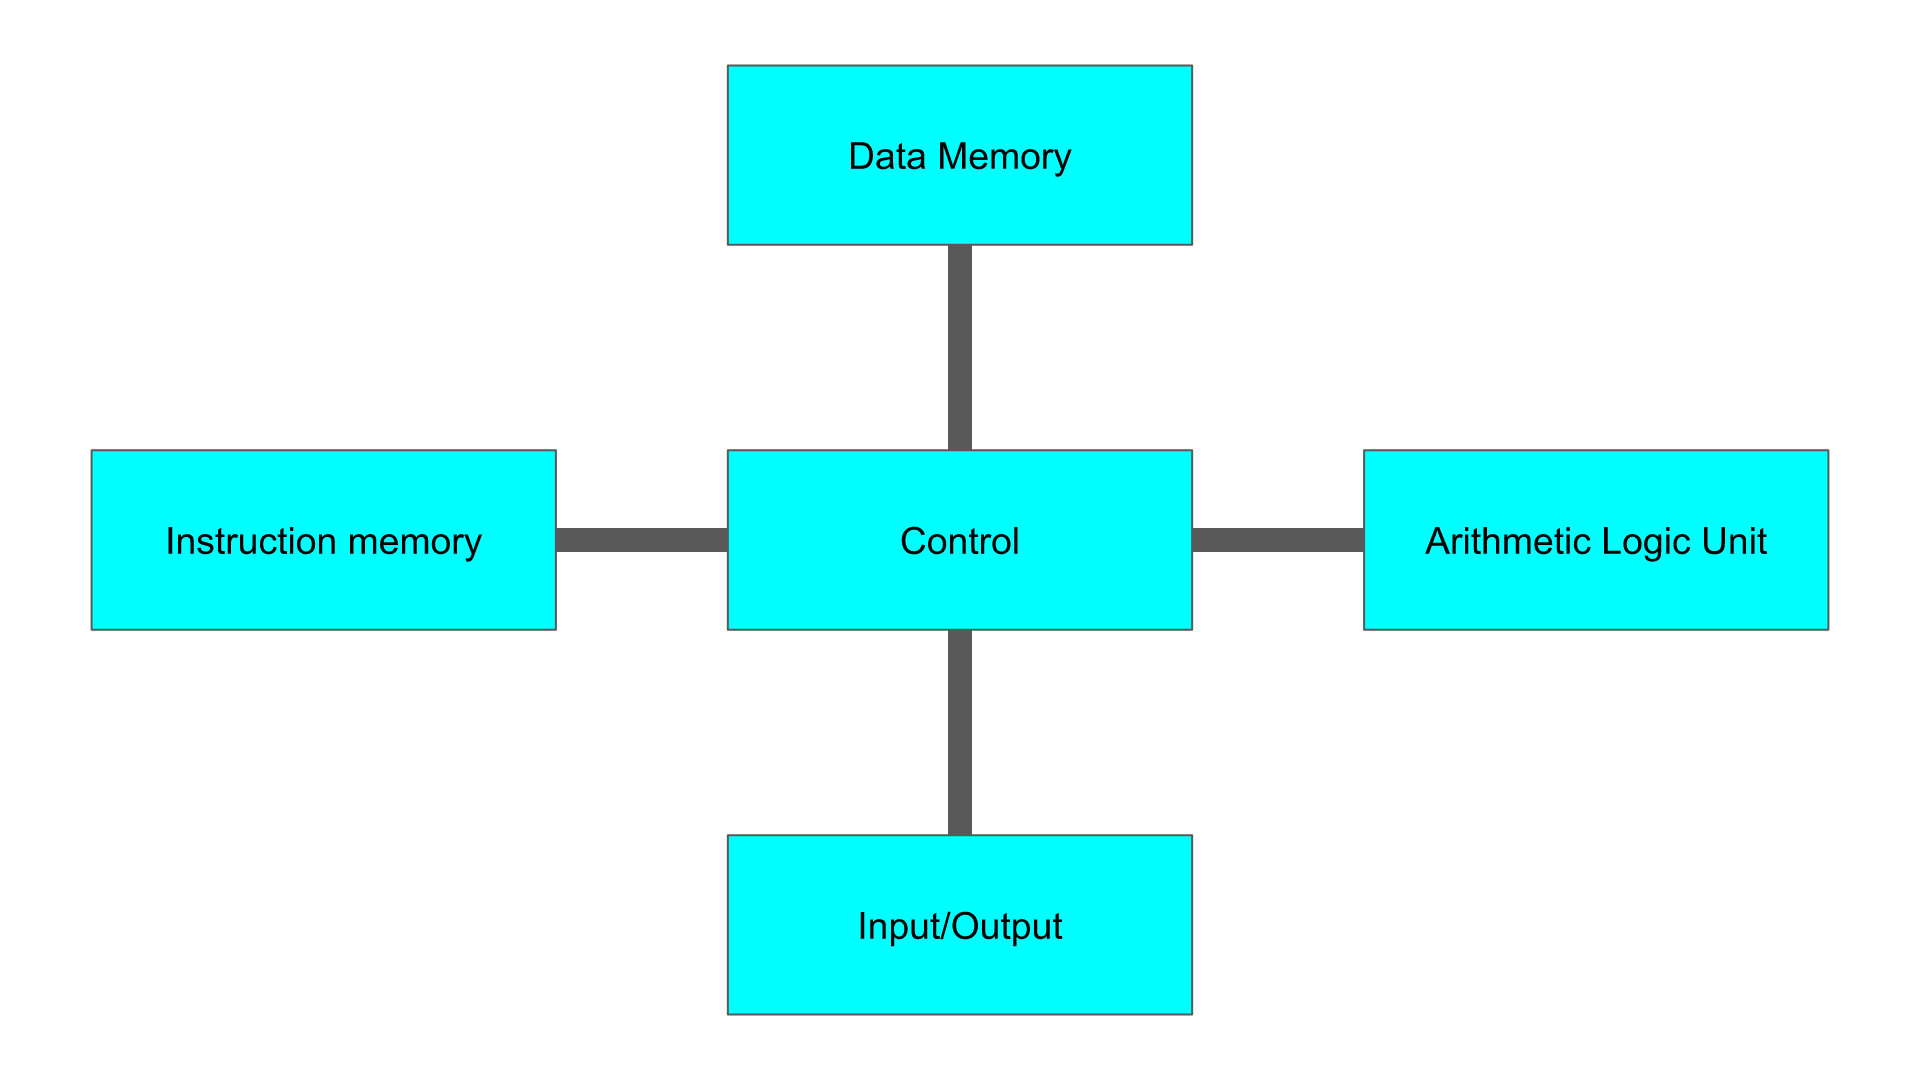
\includegraphics[width=0.8\textwidth]{figures/impl/harvardarch.png}
    \caption{Harvard Architecture}
    \label{fig:cpuHarvArch}
\end{figure}

The over-arching structure for quantum computers can be separated into two parts, there is the architecture and the platform. A quantum architecture has a different meaning to the traditional use of the word. Within the community, architectures is the distinction between the gate model, one-way quantum computing or topological quantum computing. A platform is the physical system that is used to build the computer such as, photonics, trapped ions, semi-conductor qubits, super-conducting qubits. 

We now discuss some of the current physical approaches to building a quantum computer. In reality the quantum architectures and platforms are not completely separate, some physical systems are much better suited to specific architectures. For example the gate model is a natural choice when using trapped ions or superconducting qubits whereas photons are much better suited to one-way quantum computing. 

There are two distinct types of qubits, stationary (e.g. Trapped ions or superconducting qubits) or flying qubits (photons). Here we will only discuss trapped ions and photons \textbf{Poisson Bullets are the best!!1!} as we believe these systems are the easiest to visualise conceptually. 

A good way to think of a quantum computer is a very large, noisy machine which is incredibly sensitive to its environment. The aim is trying to control it just to keep the machine coherent. Most of the resources used are for error correction, keeping the whole thing coherent, a very small part of the whole machine is the information processing. 

% what are the qubits
\subsection{What are the qubits?}

\subsection{What are the operations?}

%%%%%%%%%%%%%%%%%%%%%%%%%%%%%%%%%%%%%%%%5555
\subsection{Trapped Ions}

Trapped ions are a remarkably stable physical system (once an ion is trapped it remains trapped with a very high probability). Electric fields are used to trap the ions, by changing the voltages in the x,y,z components in the electric field it is possible to shuttle the individual ions around. This enables a great deal of control over the dynamics of the ions.

The quantum gates are performed on the qubits using either microwaves which use atomic transitions or optical pulses for electronic transitions. The microwave gates are appealing as it opens the possibility of addressing multiple qubits at once. This will be necessary when taking into account error correction as one logical X operation could correspond to 100s or 1000s of X operations on physical qubits to produce one logical X. 

The \cite{lekitsch2015blueprint} blueprint suggests using a modular approach of packing tiles shown in \autoref{fig:iontrap} on a 2D surface. Each tile would contain one ion and have a dedicated loading zone, an entangling zone with adjacent tiles each with only one ion on and a detection zone for readout. Entangling gates or operations are performed by bringing two qubits close together. This is relatively easy for trapped ions as of the good control available. 

\begin{figure}[h]
    \centering
    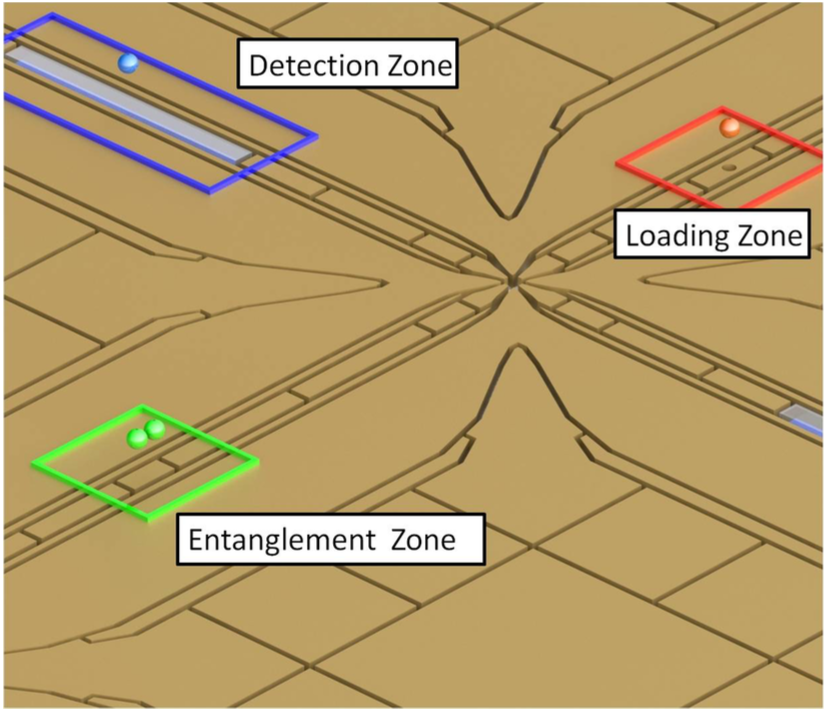
\includegraphics[width=0.6\textwidth]{figures/impl/iontrap.png}
    \caption{Caption \cite{lekitsch2015blueprint}}
    \label{fig:iontrap}
\end{figure}

%%%%%%%%%%%%%%%%%%%%%%%%%%%%%%%%%%%%%%%%%%%
\subsection{Superconducting qubits}


%%%%%%%%%%%%%%%%%%%%%%%%%%%%%%%%%%%%%%%%%%%%
\subsection{Linear optical quantum computing}

linear optical quantum computing is great! 

\begin{figure}[h]
    \centering
    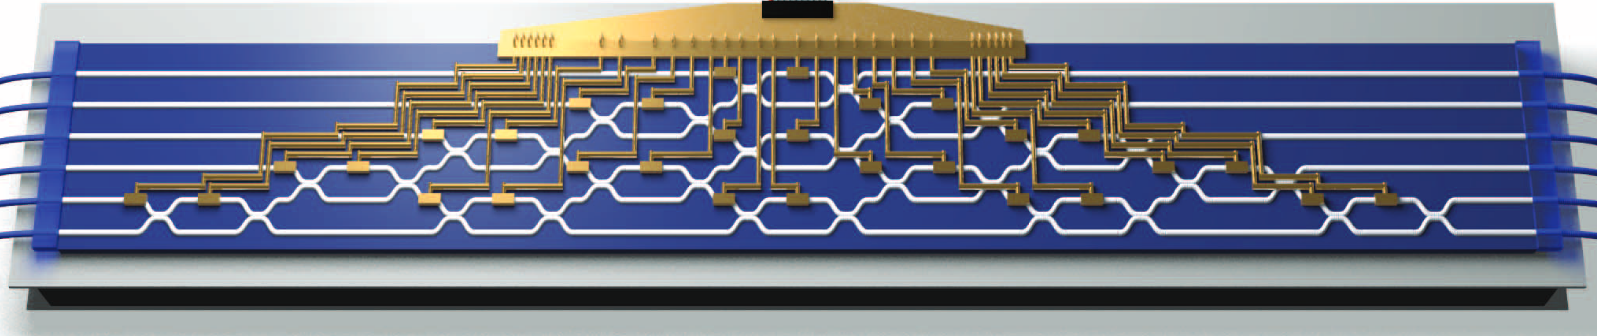
\includegraphics[width=0.6\textwidth]{figures/impl/rekkchip.png}
    \caption{Caption \cite{carolan2015universal}}
    \label{fig:my_label}
\end{figure}


%%%%%%%%%%%%%%%%%%%%%%%%%%%%%%%%%%%%%%%%%%%%
\subsection{Error Correction}

Full fault tolerance is beyond the scope of this guide however we will briefly discuss error correction. The basic idea of error correction is to use redundancy to counteract errors. Increasing the resources devoted to storing the logical information should in principle make the computer more resilient to errors.


\begin{comment}
--- PLAN ---

Focus on implementation of quantum programming languages

Implementing quantum computers:
\begin{itemize}
\item Comparison of quantum and classical computer architectures
Classical computer architectures: ALU, CPU, buses, memory, instructions, etc equivalents for quantum computers? Quantum architectures: gates? Cluster states? Quantum vs. Classical control? What are the analogues of instructions, execution, buses and memory? Are there fundamental limits to architecture design (imposed by eg no cloning. Does memory make sense in the same way as for classical computers? Quantum memory is more like single-use working-registers). How about classical computers with quantum instructions? What about qbranch instructions?   
\item Different quantum computing platforms 
Probably just a few -- maybe linear optical quantum computers and iron traps. 
\item Classical language compilers
\end{itemize}
Implementing quantum programming:
\begin{itemize}
\item Quantum error correction
Not entirely analogous to classical computers, (no instruction execution errors). Can error correction be abstracted away from the compiler level? Would error correction take place at the equivalent level of (say) instruction pipe lining in a classical processor?    
\item Quantum language compilers
What is the quantum equivalent of object code? Does it contain machine code (instructions to be executed, analogous to classical computers) or does it compile into an arrangement of gates, or some other computation mode (measurements in a cluster state?). The architecture of the quantum computer would probably heavily inform the structure of low level languages. (For example, C has basic structures essentially based on mov, branch, and arithmetic and bit manipulation instructions). Hence the low level languages of gate based quantum computers will be based on structures easily realised using gates (the gates themselves, presumably analogous to bit manipulation; coherent arithmetic, (implemented using gate arrangements lifted from half and full adders); flow control -- presumably classical; and strict mov operations, ie excluding copy). Low level languages targeted at cluster state implementation will have cluster state measurements as primitive operations (equivalent to bit manipulation) in the language, and presumably various other generic operations (like control, branching, etc.) What kind of optimisations does the C compiler do, and what are the equivalents in the quantum cases? 
\end{itemize}
--- PLAN ---
\end{comment}

%%%%%%%%%%%%%%%%%%%%%%%%%%%%%%%%%%%%%%%%%
%%%%%%%%%%%%%%%%%%%%%%%%%%%%%%%%%%%%%%%%%%%%%%%%%%
\section{Quantum software architecture}
% classical structure
Computer languages are influenced by the structure of the computer. In classical computers, languages developed historically in order to increase abstraction and ease the task of the programmer. To begin with, assembly language replaced machine code because it is easier to remember a mnemonic like ADD rather than a string of ones and zeros representing the same thing. The C programming language was invented to make common programming constructions such as if-statements and while-loops easier to program, using machine independent syntax. C is a compiled language, meaning that it needs to be converted into machine code before it can run. There is a different compiler for each computer architecture, which converts C into the specific instructions that can be executed on that machine. 

\begin{figure}[H]
    \centering
    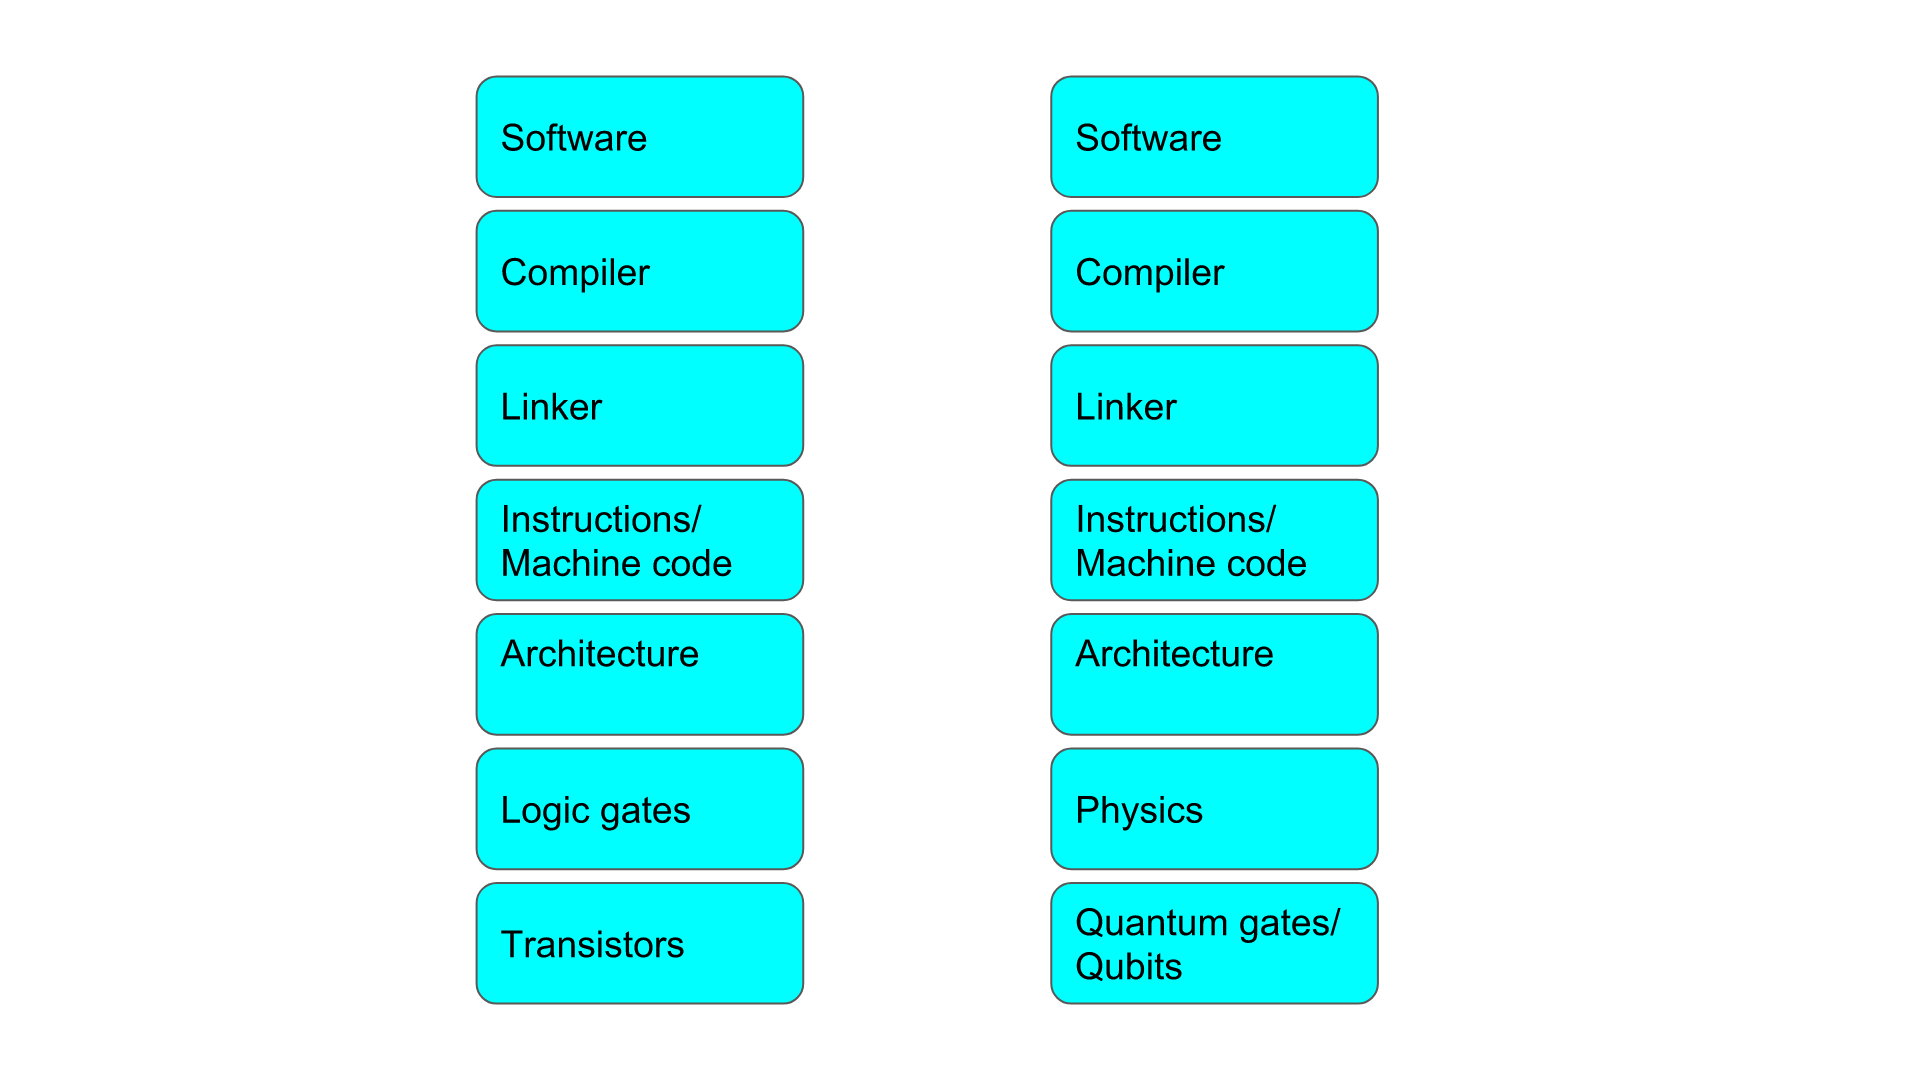
\includegraphics[width=\textwidth]{figures/impl/cpuqpu.png}
    \caption{Caption}
    \label{fig:my_label}
\end{figure}

%abstraction oop or functional
Other levels of abstraction have subsequently been introduced into programming. Some relate to code structure (object oriented programming, functional programming, and other paradigms), and others to the portability of the code. For example, Java runs in an environment called a virtual machine. This is a program which runs a file containing Java source code on a particular computer. The critical difference between this and a compiler is that many computers have a Java virtual machine, so that the end user can just run the same program without having to worry about whether there is a compiler present. 

% nisq devices birth of languages
Quantum programming languages may eventually develop in a similar way. However, there are some important differences. For example, quantum programming languages are being developed without there existing a large scale quantum computer to run programs on. This is due to the hindsight afforded by classical programming languages, and the assumption that quantum programming languages will be essentially similar. Their role is currently to understand the structure of quantum algorithms better and to provide a platform for simulating quantum computers, rather than to make programming quantum computers easier. 

% bad to do single qubits quantum computer with structure
Here, we will consider how the implementation of a large scale quantum computer might inform the structure of quantum languages. For example, most quantum programming languages currently emphasise single qubit manipulation. While this works when we only have a few qubits, it clearly becomes unfeasible in a quantum computer with a million qubits. There, it will be necessary to organise qubits into registers, variables and types depending on their role. What should those types be? How should it be informed by the structure of the quantum computer?

% re configurable logic and memory sections
Part of the issue is the current lack of understanding of large scale quantum computer architectures. A typical classical computer CPU architecture is shown in \autoref{fig:cpuHarvArch}. It contains modules for memory, processing and arithmetic, buses for moving data around, and input/output ports to connect to other devices. The computer is controlled by an instruction set, which is read and decoded in the control section. 

Each instruction performs a basic operation such as moving data from external memory into working memory, adding variables together, etc. There are also control instructions for deciding what to do next, for example branches and sub-routine calls. Memory is often organised into registers, which might be 8 bits wide in a small microcontroller, or 64 bits wide in a modern Intel processor. These instructions are the lowest level of processing available to a classical programming language. 
% 
By analogy, it is likely that a quantum computer will have a similar architecture containing an instruction set (ADD, MOV, etc.). We will consider the possible structure of such an instruction set in \autoref{sec:qinstructions}. We will then consider the simplest type of abstraction above quantum assembly language -- the analogue of C (QLang+-!). We will consider the necessity of quantum compilers and linkers, and how they differ from their classical counterparts in (section). 

%%%%%%%%%%%%%%%%%%%%%%%%%%%%%%%%%%%%%%%%%%%%%%%%%
\subsection{Quantum instruction sets}
\label{sec:qinstructions}

An instruction set is a collection of operations designed to meet two competing requirements. The instructions must contain enough operations to allow access to the full functionality of the computer, without exposing implementation details. Further, it must be simple to express a program in terms of the instruction set, so the instructions should be as high level as possible. However, the instruction set should not be overly large or contain complex operations, otherwise it would be difficult to implement in hardware.

Candidate instruction sets could therefore tend towards two opposite extremes. On the one hand, the instruction set could be very large and implement nearly everything a program might want to do: matrix multiplication, Fourier transforms, database operations, etc. Every operation would be optimised in hardware and all possible tasks would be accounted for. This would make programming and compiling very simple and programs would tend to be very efficient. However, the instruction set would be difficult to implement, and inflexible in the face of new applications and tasks.

On the other end of the scale, the instruction set might be the single operation NAND. This would be universal for classical computation, so all programs could be realised. The design of the computer would be very simple, with only one instruction to implement. However, simple programming tasks such as addition would become very difficult, and complicated programs would be nearly impossible to write.

Classical instructions sets sit between these two extremes. They contain general operations such as arithmetic (ADD, MUL, etc.), copy operations (MOV) and control flow (BRANCH, CALL, etc.) and they also contain some lower level details such as bit manipulation. 

In the rest of this section we consider the instructions which might form the basis of a full quantum computer.

%%%%%%%%%%%%%%%%%%%%%%%%%%%%%%%%%%%%%%%%%%%%%%%%%%%%%%

\subsubsection{Qubit manipulation}

Despite the need for full quantum computers to contain operations on registers, it is likely that they would retain single qubit manipulation. In classical computers single bits can be accessed using bit manipulation instructions.  For example, in the Microchip 16-bit dsPIC family of microcontrollers \cite{microchip2008AsmRef}, bits can be set to zero or one using the BCLR and BSET instructions.

\begin{lstlisting}[language=asm, caption={Single bit operations}]
    CLR     w0      ; clear register w0
    CLR     w1      ; clear register w1
    BSET    w0, #2  ; set bit #2 of register w0 to 1
    BTG     w1, #6  ; toggle bit #6 of register w1
    BCLR    w1, #5  ; clear bit #5 of register w1
\end{lstlisting}

This code initialises the two registers w0, w1 to zeroes, puts a one in the second bit of register w0, and a zero in the fifth bit of register w1. The BTG instruction toggles bit six of w2, swapping its value from one to zero or vice versa. It performs the classical NOT operation.

In quantum computers, there are many more possibilities for single qubit operations other than just setting and clearing bits. As mentioned above \textbf{REF}, a quantum computer should be able to perform all single qubit operations, which are indexed by two continuous parameters. The quantum instruction set may implement a small set of commonly used operations, such as $X$, $Y$, and $Z$. Then the assembly language may look like:

\begin{lstlisting}[language=asm, caption={Quantum X and Y operations}]
    CLR     w0      ; Quantum registers should be initialised to zero
    CLR     w1      
    QBTX    w0, #2  ; Perform an X gate on bit #2 or w0
    QBTY    w1, #5  
\end{lstlisting}

which performs an $X$ gate on the second qubit of register w0, and performs the $Y$ gate on the fifth qubit of register w1. However, the quantum computer would also need to implement arbitrary rotations and phase shifts, as follows:  

\begin{lstlisting}[language=asm, caption={Arbitrary single qubit rotations}]
    QBTX    w0, #2, #30 ; Perform a 30 degree X rotation on bit #2 of w0
    QBTY    w1, #5, #45
    QPHA    w1, #0, #45 ; Perform a 45 degree phase shift on qubit #0 of w1
\end{lstlisting}

Now, the code executes a $30\degree$ $X$-rotation on the second qubit of w0, and a $45\degree$ $Y$-rotation on the fifth qubit of w1.

The instruction set would need to contain a few 2-qubit operations, such as CNOT:
\begin{lstlisting}[language=asm,caption={CNOT operations}]
    CNOT    w0, #0, #1  ; Perform a CNOT between qubits #0 
                        ; (control) and #1 (target) of w0
    CNOT    w0, w2      ; Perform CNOT between all qubits of the
                        ; w0 (control) and w2 (target) register 
    CNOT    w0, w2, #1  ; Perform CNOT between qubit 1 of w0 and w2 
\end{lstlisting}
The CNOT operation and single qubit unitaries allow the implementation of any unitary operation on qubits. Therefore it would not be necessary to include any more two- or N- qubit gates. However, they may be included for convenience, or because they are simple to implement on a particular architecture. For example, the SWAP gate (which swaps the computational basis states) could replace the CNOT gate if it were simpler to implement a SWAP operation. 

A generalisation of the SWAP operation is the QMOV operation, which move the state of one quantum register into another: 
\begin{lstlisting}[language=asm,caption={QMOV operations}]
    QMOV    w0, w1      ; Move the quantum state of w0 to w1
    QMOV    0x1111, w1  ; Move the state stored at address 0x1111 to w1
\end{lstlisting}
This operation is more subtle than its classical counterpart. Copying is not allowed in quantum computing, so the operation would have to be realised as a swap, where the states in w0 and w1 are interchanged. Alternatively, the state might be teleported, which is a process involving measurement of register w0. The implementation of the QMOV is unimportant; the key feature is that the state which was in w0 ends up in w1.

This is actually a critical instruction of a full quantum computer. It is likely that the computer will be implemented in such a way that only a small set of register (the working registers $w_0...w_n$) support the full range of quantum operations. Therefore quantum data will need to be copied back and forth between these registers and quantum RAM, which is a large block of quantum registers whose only purpose is to store quantum states. A typical sequence of operations might be as follows:
\begin{lstlisting}[language=asm,caption={Adding }]
    QMOV    0x11FD, w1      ; Move the quantum state at address 0x11FD to w1
    QMOV    0xFFFF, w2      ; Move the quantum state at address 0xFFFF to w2
    CNOT    w1, w2          ; Perform a CNOT operation across all qubits
    QMOV    w1, 0x11FD      ; Move the states back
    QMOV    w1, 0xFFFF      ; Move the states back
\end{lstlisting}

%%%%%%%%%%%%%%%%%%%%%%%%%%%%%%%%%%%%%%%%%%%%%%%%%%%%%%%%
\subsubsection{Coherent classical operations}

Any operation which can be expressed in a classical computer has a quantum version, which we will call the `coherent' operation. A coherent operation is one that can be performed on superpositions of states. For example, addition can be implemented coherently in a quantum computer. Suppose that there are two quantum registers $\ket{a}$ and $\ket{b}$ whose contents can be interpreted as numbers. For example $\ket{0101}$ and $\ket{1001}$ represent the numbers 5 and 9. Then there is a quantum version of addition, which we will denote QADD, whose action on the states above is $$\text{QADD}\big[\ket{0101},\ket{1001}\big]=\ket{1110}.$$ In other words, it produces the state which corresponds to the result of the sum of $5 + 9 = 14$. However, it also acts on superpositions, so that $5 + 9 = 14$ and $6 + 9 = 15$ could be performed simultaneously: $$\text{QADD}\left[\frac{1}{\sqrt{2}}\big(\ket{0101}+\ket{0110}\big),\ket{1010}\right]=\frac{1}{\sqrt{2}}\big(\ket{1110}+\ket{1111}\big).$$ Now, the two possible results 14 $\ket{1110}$ and 15 $\ket{1111}$ exist in superposition in the output.

This type of operation intrinsically acts on a register containing many qubits. Otherwise it is not possible to interpret the register as a number.

The above example, QADD, is not a valid quantum operation. This is because all quantum operations must be realised as unitary operations acting on a fixed number of qubits. In particular, there must be the same number of qubits in the output of QADD as there are in the input. Implementing this process involves a complicated set of tradeoffs to do with qubit allocation and gate optimisation, as we considered in the section hardware architecture above \textbf{section}.

A valid version of QADD may work as follows:
\begin{lstlisting}[language=asm]
    QADD    w0, w1, w2  ; Add the contents of w0 and w1 and place it in w2
                        ; w0 and w1 don't change but are now entangled with w2
\end{lstlisting}
The important fact about this instruction, which makes it different from the classical version ADD, is that all three registers are considered both inputs and outputs at the same time. The QADD instruction is a unitary operations performed on the registers w0, w1 and w2. This means that w0 and w1 become entangled with w2 after the instruction has been performed.

More complicated classical operations can also be implemented coherently. Consider the function $f(x)$ of the variable $x$, which takes a bitstring of length $N$ to one of length $M$.  We want a quantum operation $Qf$ which can performs the same function as $f$, but which also acts on superpositons. For example, if $f(x)=x^2$, then $Qf$ would act as follows on the superposition of $\ket{2} = \ket{0010}$ and $\ket{0}=\ket{0000}$ as follows: $$Qf\left[\frac{1}{\sqrt{2}}\big(\ket{0010}+\ket{0000}\big)\right]=\frac{1}{\sqrt{2}}\big(\ket{0100}+\ket{0000}\big).$$ This corresponds to the fact that $2^2 = 4$ and $0^2 = 0$, and those two computations can be performed in superposition. As in the case of QADD, this operation must be implemented as a unitary operation acting on a fixed number of qubits. One way of achieving this is defining the unitary map $$\ket{x}\ket{y} \xmapsto{Qf}  \ket{x}\ket{f(x) \oplus y},$$ where $\oplus$ is bitwise XOR. Here, $x$ is a register containing the input $N$ bit number, and $y$ is a $n$ bit register. Then setting $y=\ket{0}$ results in the the value $f(x)$ being written into the $y$ register: $$\ket{x}\ket{0} \xmapsto{Qf}  \ket{x}\ket{f(x)}.$$ This operation is often called the bit oracle. 

This form of $Qf$ can also be used to implement a coherent function of two variables $g(r,s)$. Suppose that $r$ and $s$ are $N$ bits long and the output is again $M$ bits long. By concatenating $r$ and $s$, we get a single $2N$ bit long number, which we will call $x$. Then $f$ can be seen as a function of a single variable $x$, which can be implemented using $Qf$ above. 

For example, consider the implementation of QADD for 2-bit input arguments. The classical function is addition, i.e. $g(r,s) = r+s$. Concatenating $r$ and $s$ gives a new variable $x$. The truth table for the output $g$ for different values of $r$ and $s$ is shown in \autoref{tab:2bitaddtruth}.
\begin{table}[!htb]
    \caption{Truth table for 2-bit addition}
    \label{tab:2bitaddtruth}
    \begin{subtable}{.5\linewidth}
      \centering
        \begin{tabular}{|l|l||l|}
        \hline
        \multicolumn{2}{|c||}{$x$} & $f(x)$\\
        \hline
        $r$ & $s$ & $r+s$ \\ \hline
        00       & 00       & 0000       \\ 
        00       & 01       & 0001       \\ 
        00       & 10       & 0010       \\ 
        00       & 11       & 0011       \\
        01       & 00       & 0001       \\ 
        01       & 01       & 0010       \\ 
        01       & 10       & 0011       \\ 
        01       & 11       & 0100       \\
        \hline
    \end{tabular}
    \end{subtable}
    %
    \begin{subtable}{.5\linewidth}
      \centering
        \begin{tabular}{|l|l||l|}
        \hline
        \multicolumn{2}{|c||}{$x$} & $f(x)$\\
        \hline
        $r$ & $s$ & $r+s$ \\ \hline
        10       & 00       & 0010       \\ 
        10       & 01       & 0011       \\ 
        10       & 10       & 0100       \\ 
        10       & 11       & 0101       \\
        11       & 00       & 0011       \\ 
        11       & 01       & 0100       \\ 
        11       & 10       & 0101       \\ 
        11       & 11       & 0110       \\
        \hline
    \end{tabular}
    \end{subtable} 
\end{table}
Here, it is clear that the variables $r$ and $s$ can be concatenated into a single variable $x$, and that the truth table in \autoref{tab:2bitaddtruth} can be interpreted as a function of a single variable $x$ which maps 4-bit numbers to 4-bit numbers. 

Clearly a quantum computer will need enough instructions to implement all coherent operations of interest. One way to achieve this would be to implement an instruction QFUN which implements an arbitrary reconfigurable coherent operation. The truth table of the classical function could be loaded into a dedicated block of registers $f0,...,fn$. 

For example, consider the function $f(x)$ on a 2 bit variable $x$ defined by the truth table in \autoref{tab:1bitadd}. The function $f(x)$ is the classical XOR operation on 2 bits, but could also be interpreted as the 1-bit half adder (addition modulo 2).
\begin{table}[!htb]
    \caption{Truth table for 1 bit addition}
    \label{tab:1bitadd}
      \centering
        \begin{tabular}{|l||l|}
        \hline
        $x$ & $f(x)$ \\ \hline
        00  & 0      \\ 
        01  & 1       \\ 
        10  & 1       \\ 
        11  & 0       \\
        \hline
    \end{tabular}
\end{table}
This function could be loaded an implemented coherently as follows:
\begin{lstlisting}[language=asm]
    ; Set the function f(x)
    MOV     #0, f0    ; Load the truth table for f(x)
    MOV     #1, f1    ; by moving the truth table outcomes
    MOV     #1, f2    ; into the registers f0...f3
    MOV     #0, f3
    ; Perform the coherent operation
    QFUN    w0, w1      ; Here, w0 contains x. The output
                        ; y will be stored in w1.
\end{lstlisting}

This approach suffers from two key drawbacks. The first is its implementation, which may be very difficult. The hardware would need to decide how to implement the coherent operation, which is a non-trivial resource allocation problem. It would likely be quite difficult to come up with general purpose hardware which produces optimised results for all classical functions $f$. The second more serious problem is the lack of extensibility. Here, the size of the function $f$ (i.e. the number of rows in its truth table) is limited by the number of dedicated registers $f0...fn$. This is especially true of truth tables which are sparse, where most of the dedicated registers represent wasted space. 

A better approach would be to devise a minimal set of instruction which could be used to realise all coherent classical operations. For example, suppose that QADD and QMUL were implemented as follows:
\begin{lstlisting}[language=asm]
    MOV     #2, w0      ; 
    MOV     #3, w1   
    QADD    w0, w1, w2  ; Add 2 by 3 and put the result (5) in w2
    QMUL    w0, w1, w3  ; Multiply 2 by 3 and put the result (6) in w3 
    QADD    w2, w3, w4  ; Add the contents of w2 and w3
\end{lstlisting}
These kind of manipulations can be used to build up any polynomial coherent operation. 

An interesting implementation of the quantum adder is presented by Draper \cite{draper2000addition}. The circuit makes use of the Quantum Fourier Transform to turn addition operations into phase operations, and then uses controlled phase gates to implement the operation. This approach avoids using the carry qubits which are involved in implementing addition based on classical models of addition. The same type of approach is extended by Beauregard \cite{beauregard2003ShorImplementation} to obtain the coherent multiplication operation.

% The paper describes a way of implementing a^x mod N using coherent arithmetic. It should be easy to write assembly for the operation below.

%%%%%%%%%%%%%%%%%%%%%%%%%%%%%%%%55 
\subsubsection{Quantum conditionals}

One of the most important operations in classical computing is the if-statement. This is a control flow operation, which checks whether a condition is true and executes one block of code or another accordingly.

The prototypical conditional operation in many instruction sets is the bit test. For example, BTSC (bit-test skip-if-clear) can be used to implement the classical controlled-NOT gate, with the truth table 
\autoref{tab:classCNOT}.
\begin{table}[!htb]
    \caption{Truth table classical CNOT}
    \label{tab:classCNOT}
      \centering
        \begin{tabular}{|l||l|}
        \hline
        $x$ & $f(x)$ \\ \hline
        00  & 0      \\ 
        01  & 1       \\ 
        10  & 1       \\ 
        11  & 0       \\
        \hline
    \end{tabular}
\end{table}
The operation is performed by testing whether the control bit A is one, and if it is toggle bit B (using BTG). If A is zero, the BTSC causes the BTG line to be skipped.
\begin{lstlisting}[language=asm]
    BTSC    w0, #0 ; comment
    BTG     w0, #1
\end{lstlisting}

In quantum instruction sets, there will almost certainly be classical branching operations, which perform quantum operations that are conditioned on the value of classical bits. However, it is conceivable that there are also quantum conditional operations, where the BTSC instruction above might be generalised to depend on a qubit. For example, the QBTSC instruction would execute the next line of code if the test qubit is in the state one, otherwise the next line would be skipped.

What if the test bit is in a superposition of zero and one? Then the outcome of the program should be to leave the quantum computer in a superposition of executing and not executing the next line of code.

For example, the CNOT gate could be implemented as follows:
\begin{lstlisting}[language=asm]
    QBTSC   w0, #0
    QBTG    w0, #1
\end{lstlisting}
Here, the target (qubit 1 of w0) is toggled depending on the value of the control (qubit 0 or w0). If the control is in the state $$\frac{1}{\sqrt{2}}\big(\ket{0}+\ket{1}\big),$$ then the target would be in a superposition of non-toggled and toggled -- exactly the action of the CNOT gate. 

% Add a section about quantum conditional branching
\begin{comment}
Such an operation could be used to implement the coherent operation of exponentiation, $f(x) = a^x$, where $a$ is some fixed integer and $x$ is a quantum register. The algorithm works by repeatedly multiplying $a$ by itself. Each time $a$ is multiplied by itself, the $x$ register is decremented 
\begin{lstlisting}[language=asm,caption={Compute $a^x$ for $a=3$}]
    ; Set w2 as a superposition 
    MOV     #3, w0  ; Copy a=3 into w0
    MOV     #1, w1  ; Start with #1 in w1
    ; Assume w2 contains x 
A:  QRTBC   w2, B       ; Branch to B if w2 is 0
    QMUL    w1, w0, w1  ; Multiply w1 by w0 and store result in w1 
    QDEC    w2          ; Decrememt w2 by 1 (w2 = w2 - 1) 
    BRA     A           ; Branch to A
B:                  ; w2 now contains 3^x
\end{lstlisting}

\url{https://docs.google.com/presentation/d/1SAYwmZ2yAanG0IhbPK4y2j\_JfoOjs\_K9bXPlLtm7Q0w/edit?usp=sharing}

%https://arxiv.org/abs/1311.1074

\end{comment}

%%%%%%%%%%%%%%%%%%%%%%%%%%%%%%%%%%%%%%%%%%%
\subsubsection{Measurement instructions}

One of the most important features of quantum computing is the ability to measure qubits and collapse the state to one of a particular set of outcomes. Measurements can be made in arbitrary bases, but these can always be reduced to measurement in the computational basis by a suitable choice of single qubit unitary operations. 

The following example shows some possible measurement instructions
\begin{lstlisting}[language=asm,caption={Quantum register measurement}]
    QMEAS   w0, cw1     ; Measure quantum register w0, place result in classical register cw1
    QMEAS   w1, #0, cw1 ; Measure qubit 0 of w0, place the result in cw1
\end{lstlisting}

%%%%%%%%%%%%%%%%%%%%%%%%%%%%%%%%%%%%%%%%%5
\subsubsection{Classical operations}

It makes sense for the instruction set of a quantum computer to contain classical operations as well. Many quantum algorithms (e.g. Shor's factoring algorithm, the variational quantum eigensolver), contain both quantum and classical elements, and so it would be benificial to be able to access both types of operation in the same machine using a consistent syntax. 

This entails the encorporation of many instructions which are standard on classical computers: for example, arithmetic (ADD, MUL), control flow (CALL and BRA), bit manipulation, etc. As discussed in the hardware section \textbf{above}, these would be implemented by classical logic in the classical part of the quantum computing architecture. 

In addition to purely classical operations, some instructions could have hybrid quantum/classical dialects. For example, the addition instruction QADD could add two quantum registers or add a quantum register to a classical register:
\begin{lstlisting}[language=asm,caption={Different dialects of QADD}]
    QADD    w0, w1, w2  ; Add quantum registers w0 and w1 and 
                        ; place result in w2
    QADD    cw0, w0, w1 ; Add classical register cw0 to quantum                      
                        ; register w0 and place the result in w1

\end{lstlisting}
This kind of thing, where a single instruction can take many different types of arguments, is standard in classical instruction sets. Behind the scenes, the instructions might be implemented differently depending on their arguments. For example, as described by Beauregard \cite{beauregard2003ShorImplementation}, it is possible to reduce the number of quantum gates required for adding a classical register to a quantum register, compared to the full operation of adding two quantum registers.


%%%%%%%%%%%%%%%%%%%%%%%%%%%%%%%%%%%%%%%%%
\subsubsection{Quantum types}
The most important of these is a quantum type. Classical types typically include things like `double' (for integers), `char' (for letters), `float' (for floating point number), etc. and possible more complex types like point (which contain references to variables). In a quantum computer, there would have to be a types for a quantum registers. For example, `qdouble' might refer to a quantum register whose contents is interpreted as an integer. A `qbitmap' might refer to a register whose contents is not to be interpreted, i.e. all the qubits should be treated independently.

There would probably not be a qubit type in quantum languages for long-term quantum computers. This is because there would presumably be enough resources that a quantum register (say 8 qubits wide) could be used as a single qubit, but ignoring the other seven qubits. This is similar to the lack of a bit type in modern classical programming languages, for the same reason.

%%%%%%%%%%%%%%%%%%%%%%%%%%%%%%%%%%%%%%%%%
\subsubsection{Quantum operations}
There would need to be fundamental quantum operations. The types of quantum operations would be dictated by the quantum type of the variables which are operands. For example, two variables of type qdouble could be coherently added, but it would not make sense to coherently add two variables of type qbitmap.

There would need to be some facility for implementing quantum measurements. There would need to be some variant of a `measure' keyword, which could be made to either measure registers of single qubits. This might depend on type, so that by default qdouble are measured register wide but qbitmaps require an argument specifying which bit to measure.

There is also the possibility of including quantum conditional operations, such as a quantum if statement. Ignoring for the moment the (extreme) difficulty of implementing such a construction, there are several ways the syntax might work. One is to have a standard if statement which automatically becomes as classical or quantum if depending on the type of the argument. Alternatively, there may be two keywords, cif (classical-if) and qif (quantum-if), which make the distinction obvious in the source code.  

%%%%%%%%%%%%%%%%%%%%%%%%%%%%%%%%%%%%%%%%%%
\subsection{Higher level languages}

The purpose of higher level languages is to provide a readable syntax for common language constructions. These can then be translated by a compiler into assembly language for a particular machine. This removes the need for the programmer to understand machine code, and also makes the language portable across platforms with different instruction sets. 

In classical computing, high level programming languages contain control flow statements (if, for, while, etc.), type checking (e.g. whether a register is interpreted as an integer or a character), syntax for defining functions, etc. 

In a quantum programming language, many of these remain. It would still be of interest to perform classical operations such as classical if-statements and classical function calls. However, there would need to be new features to account for the new quantum elements that are accessible to the programmer, as we describe below.

%%%%%%%%%%%% %%%%%%%%%%%%%%%%%%%%%%%%%%%
\subsection{High- and low- level quantum languages}

functional vs object oriented. High level languages is all about adding abstraction: language constructs are not closely related to computer hardware features, but should be easier/more intuitive to use, and should work across different hardware implementations.

Low level languages:more quantumness, harder to use, but more closely related to hardware and consequently not portable. E.g. assembly based on the instruction set architecture, C constructs are based closely on instructions (if, while, do, based on branch instructions. arithmetic, bit manipulation, variable storage and access are all cpu instructions).

%%%%%%%%%%%%%%%%%%%%%%%%%%%%%%%%%%%%%%%%%%%%%%%%%%%%%
\subsection{Examples of different types of languages}

Discuss the languages included in the language section: Q\#, Quil, Quiskit, Scaffold \footnote{C}. 

The majority of currently available quantum languages are (high level languages with object oriented structure such as Python and C\# but are used as low level languages). As discussed in section \textbf{REF} the languages reduce to listing quantum gate instructions, building up the logic circuit for the algorithm by essentially by hand. This can pose problems for algorithms which make use of a quantum oracle which is a unitary $U(f(x))$ which depends on a classical function $f(x)$ as calculating an optimal reversible version of $f(x)$ is hard classically to compute \textbf{REF (p polling)}.

Python is an interpreted and C\# uses JIT compilation, Scaffold resembles the most compiled language present in our discussion. 

The current languages discussed here use individual qubits focusing on the ability to address each qubit individually. We hope that future languages will avoid doing this as it poses problems for many qubit machines.

%%%%%%%%%%%%%%%%%%%%%%%%%%%%%%%%%%%%%%%%%%%%%%%%%%%%%
\subsection{Compilers}

Compilers break down programming language code into the instruction set of the machine. The compiler is more or less important depending on the amount of abstraction in the language. The difficulty of implementing the compiler depends directly on how much abstraction is already contained in the instruction set. By definition, assembly language does not require a compiler because it is already written in terms of machine instructions. At the moment the machine code of all existing quantum information processors is their gate set, meaning that the compiler must perform gate synthesis (see \autoref{physimp} for a more detailed discussion on gate synthesis). 

This is contrary to the implementation of classical computers, whose instruction set is a much higher level than logic gates. We anticipate that large scale quantum computers will eventually have instruction sets that contain many more quantum operations in addition to quantum gates, meaning that the burden on the compiler will be greatly reduced.

review compiler progress with references. Include the `compiler' for pyquil. comment on the range of meanings `quantum compiler' seems to have. Are there any actual compilers? Is the scaffold compiler legit?

language design what about quantum computing as a whole influences the design of the language for future languages. How does the quantumness show up at different levels of abstraction (i.e. gates at the bottom, quantum-if statements a bit of the way up, ..., languages with no explicit references to quantum stuff?)

%%%%%%%%%%%%%%%%%%%%%%%%%%%%%%%%%%%%%%%%%%%%%%%%%%%%
\subsection{Linkers}

Oli's fault not finished.
connectivity, memory allocation (qubit allocation),  

%%%%%%%%%%%%%%%%%%%%%%%%%%%%%%%%%%%%%%%%%%%%%%%%%%%%%
\section{The future}


\subsection{QLANG $+-$ \textsuperscript{TM} the Quantum programming language}

We introduce the QLANG$+-$\textsuperscript{TM} language qubytes\textsuperscript{TM} and quibbles\textsuperscript{TM}. 
  

%%%%%%%%%%%%%%%%%%%%%%%%
\bibliographystyle{unsrt}
\bibliography{References}

%%%%%%%%%
\appendix

%%%%%%%%%%%%%%%%%%%%%%%%%%%%
%\chapter{Advanced topics}
\chapter{A gentle introduction to quantum theory}
\label{chpt:advancedtopics}

In this chapter we cover some supplementary background quantum theory. Although a deeper knowledge of quantum theory would serve to further your understanding of quantum computing, everything you need to know for this guide is covered in \autoref{chpt:background}. The following textbook is referenced throughout this Appendix which we recommend to interested readers: \textit{"Quantum Computation and Quantum Information"} by M. A. Nielsen and I. L. Chuang \cite{nielsen_chuang_2010}. You have seen in Section \autoref{chpt:background} that the state of a system governed by quantum mechanics can be represented by a sum of basis states that each correspond to binary representations of information. In this section we will give a more detailed introduction to Dirac notation and cement the description given in Section \autoref{chpt:background} into a more formal language that will allow you to describe more complex systems and will allow you to probe deeper into more advanced literature.


\section{Quantum States}

In quantum mechanics, we describe the state of a system simply with labels. These labels we assign to the system, such as {`0',`1'}, aim to give some intuition about the state of the system. We could equally have used {`open', `closed'} if appropriate. This labelling should be viewed as assigning information to a state. For example, if a state is labelled '110' then in binary representation, the state carry's the information '6'. Formally these labels are called quantum numbers and in general can be anything you like.\\

For example, imagine the 4 of spades was chosen from a deck of cards, a good choice of label to describe the card would be `4' or `$\spadesuit$'. Equally in a quantum system we would say that the card is in the state `4' or `$\spadesuit$' which we write formally as $\ket{4}$, or $\ket{\spadesuit}$. In this scenario the quantum number `4' of the chosen card could have been one of 13 possible values, therefore the set of states needed to fully describing the system (the system here being a randomly chosen card from a single deck of cards) are $\{\ket{A}, \ket{2}, \ket{3},\ldots ,\ket{K}\}$ with quantum numbers $\{A,2,3,\ldots K\}$. If the set of quantum numbers are unique and their associated states describe all possible values a properties can take then they are said to form a Hilbert space $\mathcal{H}$ of the system \cite{nielsen_chuang_2010} \textit{p66}. Formally we say the complete set of independent and orthonormal states describing a system span a Hilbert space of that system:

\begin{equation}
\mathcal{H}:=span\{\ket{A}, \ket{2}, \ket{3},\ldots ,\ket{K}\}
\end{equation}

A Hilbert space is a vector space with a defined inner product. Its purpose is to mathematically define all the possible states a system can occupy. This is a very useful tool when we start to describe the evolution of a system because it had better be the case that our description of a system remains physically possible, i.e. remains within the Hilbert space. For example, it would make no sense to talk about the state $\ket{A}$ evolving to the state $\ket{18}$ as there are now cards valued that high in the deck. In that sense, the Hilbert space helps define the boundaries of a system.\\

As described in \autoref{chpt:background}, $\ket{\ldots}$, used to describe a state, is called a `ket'. For every `ket' there is a `bra' conversely written as $\bra{\ldots}$. The names originates from the first and second halves of the word `bra(c)ket', which when placed together resemble the most important operation in quantum computation: the inner product. For a formal introduction to Dirac notation \textit{see p13} of \cite{nielsen_chuang_2010}. The inner product is a simple function that does the following on \textit{basis} states in the Hilbert space:\\

\textit{if (state $\ket{a}$ is the same as state $\ket{b}$)\\ 
    return 1 \\
else \\
    return 0}\\ 

In Dirac notation this operation is performed by finding the associated bra of the state, $\bra{a}$ (this process is described more formally in Section \autoref{superposition} but for now can be thought of as just a bracket swap). The `bra' $\bra{a}$ and `ket' $\ket{b}$ are then used to form the word `bra(c)ket' and is equal to 1 or 0 depending on whether the state a is equal to the state b.\\

For example, returning to our deck of cards, the inner product of the states $\ket{A}$ with $\ket{5}$ is written as:

\begin{equation}\label{Example_Inner_Product}
\bra{A}\ket{5} = 0
\end{equation}

Conversely, the inner product of the states $\ket{J}$ with $\ket{J}$ would be:

\begin{equation}
\bra{J}\ket{J} = 1
\end{equation}

When a set of states are unique in this way, they are said to be orthonormal. The inner product is important as it allows you to check that all the states that form your Hilbert space are orthonormal (remember this is a key requirement for a set of states to form a Hilbert space) and will become very useful when we introduce superposition in the next section.\\

It should be noted that the dimension of a Hilbert space is equal to the number of basis states that span it. In the case of our deck of cards, the Hilbert space of card values has dimension 13. Binary representation of information only increase in dimension size by powers of 2 meaning the full Hilbert space would have dimension size that is also a power of two. Typically in quantum computing we only deal with qubits which on there own have 2 dimensional Hilbert spaces spanned by $\ket{0}$ and $\ket{1}$. As a result, when two qubits are combined, their joint Hilbert space has $2^2$ basis states spanned by ${\ket{00}, \ket{01}, \ket{10}, \ket{11}}$. In this way, it will always be possible to capture the Hilbert space of $n$ qubits with a binary representation of $2^n$ labels. Composite systems of Hilbert Spaces will be discussed further in the following Section.

\section{Superposition}

Using the states that form the basis of our Hilbert space to describe the system is not sufficient. Observation of quantum systems tell us that when we prepare a state multiple times and measure it, the outcome will not always be the same but instead follow some probabilistic statistics. At this point its crucial to point out that the formalism does not try to explain why this is the case, but only provides a way of describing the system. We highlight this fact for the following reason. Typically when confronted with a new phenomena, we turn to the mathematical description to gain some intuition of its causes. With quantum mechanics, the formal description should not be used to find a "logical" explanation of how superposition works but only used to help fully describe the observed physics of the system.\\

To understand how we can describe this phenomena formally, lets make our deck of cards a quantum deck of cards that now obeys the laws of quantum mechanics and see how our observations are captured within the mathematical formalism.\\

The first thing to note is that the act of measuring appears to perform an operation on the system that takes it from its superposition state to a basis state of the Hilbert space. The pre-measurement `superposition state' contains information about which outcomes we will attain and with what probability we will attain each measurement outcome.\\

For example, lets say you are given a face down card that when flipped multiple times is sometimes a queen and sometimes a 4 (strange, but totally allowed within quantum mechanics). Before performing the operation of turning it over the state of the card should be thought of as being in a superposition of $\ket{Q}$ and $\ket{4}$. That is to say, the state used to describe the system before the measurement operation is not just one basis state but two, containing some probabilities that describe how often we get each outcome. Only under the measurement operation (in this case the act of flipping the card) does the state become one of the two basis states. In general we may not be aware of how likely each outcome is and so to build up a picture of the superposition state we must re-prepare the experiment and repeating the same measurement many times. Since all we have to describe the systems pre-measurement state is the probabilities of getting each state after measurement, this is what's use in the mathematical description.\\

Formally, given a state $\ket{\psi}$ that is said to be in a superposition of the states $\ket{a}$ and $\ket{b}$ where the probability of getting the state $\ket{a}$ is $\abs{\alpha}^{2}$ and the probability of getting the state $\ket{b}$ is $\abs{\beta}^{2}$ then we describe the state as:

\begin{equation}
\ket{\psi} = \alpha \ket{a} + \beta \ket{b}
\end{equation}

In general, both $\alpha$ and $\beta$ can take complex values and so to ensure that the probabilities are real we take the absolute value squared (see \cite{nielsen_chuang_2010} \textit{p80} for an example of how to take the absolute value). The significance of having complex valued amplitudes will be discussed on the next page but for now it's sufficient to consider them as real.\\

Returning to our example, say we get a queen one third of the time and a four two thirds of the time. We would describe the pre-measurement superposition state as:

\begin{equation}
\ket{\psi} = \frac{1}{\sqrt{3}} \ket{Q} + \frac{2}{\sqrt{6}}  \ket{4}
\end{equation}

where

\begin{equation}
\abs{\frac{1}{\sqrt{3}}}^{2}+ \abs{\frac{2}{\sqrt{6}}}^{2} =1
\end{equation}

as expected since the probabilities of getting a queen or a four must sum to one. It is true that $\ket{\psi} \in \mathcal{H}$ since any linear combination of the basis states lives within the span of those basis states. 
\subsubsection{Aside: Why do we use complex amplitudes?}
\hrule
\vspace{\baselineskip}
In general the amplitudes $\alpha$ and $\beta$ are used not only to keep track of the probabilities of possible measurement outcomes, but also to account for a second important property, namely, the relative phase between each state. The need for a phase, as well as a magnitude, originates from our observations of wave-like interference between two superposition states. From experimental observations we know that quantum mechanical particles (even particles with mass) have inherent wave like properties such as wavelength and phase that must be reflected within the mathematical description. Each basis state in the superposition has a relative phase that helps describe how the overall state will constructively or destructively interfere when combined with another state. For a review of the general postulates of quantum mechanics see \cite{nielsen_chuang_2010} \textit{p96}.\\
\hrule
\vspace{\baselineskip}

Complex numbers are useful because they naturally contain a phase. Each complex number can be parameterised as $\alpha = \abs{\alpha}e^{i\theta}$ where the angle $\theta$ is the phase angle that can take any value between 0 and $2\pi$. To help see the significance of the phase let's look at the difference between two states with different phases such as: $\ket{\psi_{a}}=\frac{1}{\sqrt{2}}(\ket{0}-\ket{1})$ and $\ket{\psi_{b}}=\frac{1}{\sqrt{2}}(\ket{0}+\ket{1})$. Both are superposition's of the state 0 and 1 with equal probabilities but with different relative phases preceding the 1 state (note that $e^{i\pi}=-1$). The relative phase difference will manifest itself when the two states interfere with each other, the result of which can be seen by taking the inner product between them just as before, except now the states are superposition states with complex amplitudes instead of basis states. Lets take this opportunity to introduce a more formal definition of the inner product of two arbitrary states and practice how to perform such a product.\\

To compute the inner product we take the 'bra' of $\ket{\psi}$ as before in Example \ref{Example_Inner_Product} except now the 'bra' of $\ket{\psi}$ is given by the complex conjugate of the amplitudes multiplying the basis states within $\ket{\psi}$. For example, given $\ket{\psi}=(\alpha\ket{a}+\beta\ket{b})$ and $\ket{\phi}=(\gamma\ket{a}+\rho\ket{b})$ where $\{\alpha, \beta, \gamma, \rho\} \in \mathbb{C}$ then $\bra{\psi}=(\overline{\alpha}\bra{a}+\overline{\beta}\bra{b})\equiv (\ket{\psi})^\dagger$. More formally the process described above is called 'taking the adjoint' of the state and is signified by the dagger.
The complex conjugate of a complex number (denoted by an overhead bar) is given by simply negating the complex part. For example, if $\alpha=a+ib$ then the complex conjugate is given by $\overline{\alpha}=a-ib$. The `bra' is then used with the `ket' to form `braket' just as before in Example \ref{Example_Inner_Product}. Since the inner product is a distributive operation, the `braket' can be expanded out just as in normal multiplication making sure each `bra' is combined with every `ket':\\

\begin{equation}
\begin{split}
\bra{\psi}\ket{\phi}&=(\overline{\alpha}\bra{0}+\overline{\beta}\bra{1})(\gamma\ket{0}+\rho\ket{1})\\
&=(\overline{\alpha}\gamma\bra{0}\ket{0}+\overline{\alpha}\rho\bra{0}\ket{1}+\overline{\beta}\gamma\bra{1}\ket{0}+\overline{\beta}\rho\bra{1}\ket{1})\\
&=(\overline{\alpha}\gamma+\overline{\beta}\rho)
\end{split}
\end{equation}

For example, using $\ket{\psi_{a}}$ and $\ket{\psi_{b}}$ given above, the inner product is as follows:

\begin{equation}
\begin{split}
\bra{\psi_a}\ket{\psi_b} &= \frac{1}{2}(\bra{0}-\bra{1})(\ket{0}+\ket{1})\\
&=\frac{1}{2}(\bra{0}\ket{0}+\bra{0}\ket{1}-\bra{1}\ket{0}-\bra{1}\ket{1})\\
&=\frac{1}{2}(1+0+0-1)\\
&=0
\end{split}
\end{equation}

We can see above that due to the minus phase on the basis state $\ket{1}$ in the superposition state $\ket{\psi_a}$ the inner product is 0, or in other words, when combined the overlap of the two superposition states destructively interfere giving a zero inner product i.e. the two states are orthogonal to each other. Had the phase been different, the inner product could have taken a non-zero complex value signifying some constructive interference between them. For a more in-depth discussion of superposition see \cite{nielsen_chuang_2010} \textit{p13}.

\section{Operators}

So far we have discussed how to formally describe the state of a quantum mechanical system and how to calculate the probability of a measurement outcome on a superposition state. We also introduced the notion of a measurement being a type of operation that maps superposition states to basis states. In general, all measurements are represented by \textit{Hermitian} operators that have some specific properties. General quantum mechanical measurement is beyond the scope of this guide and instead we will restrict our discussion to the computational basis state $\{\ket{0}, \ket{1}\}$ used in quantum computation to describe qubits (see \cite{Busch1996} for a more general discussion of measurement in quantum mechanics). In this restricted case, a measurement determines the value of the qubit (0 or 1) with some probability determined by the state it's in. \\

An operator can be thought of as a mapping of one state to another, like applying a BIT-FLIP to the basis states in a superposition or even the mapping of a basis state into a superposition state. These types of simple operation form the basis of all quantum computation, much like AND, OR and COPY in classical computation, except now the rules are different. One key difference is that there is no COPY operation since in order to copy a state, it must first be measured. The issue is that measuring collapses (or projects) a state to a basis state so we can never know the exact form of the pre-measurement state and therefore cannot make a true copy. We can express the idea of a general operation by the following equation:

\begin{equation}
    \ket{\phi}=\hat{O}\ket{\psi}
\end{equation}

The most trivial operator we can imagine is the identity operator $\hat{I}$ that just maps a state $\ket{\psi}$ to itself. In order to remain physically reasonable the operator $\hat{O}$ has a number of important restrictions that are listed and explained below.

\begin{enumerate}
  \item $\hat{O}:\mathcal{H}\rightarrow \mathcal{H}$. The operator must map states of a Hilbert space to other states in the same Hilbert space. Remember that the Hilbert space defines the boundaries of our physical system which must be respected as we are considering only closed systems. 
  \item The operator must preserve the inner   products between the basis states.
    This is the same as saying that an operator cannot change the fundamental nature of the basis states. For example, the 0 and 1 state must always be orthonormal to each other otherwise they will no longer form the Hilbert space and the boundaries of our system will then change. This results in the equality $\hat{O}^\dagger\hat{O}=\hat{I}$ (we will see what the adjoint of an operator is shortly). Interestingly, for the above to be true the operator must have an inverse and therefore must be reversible.
\end{enumerate}

Operators are mathematically represented in the computational basis by a string of back to back `kets' and `bras'. This form allows the mapping of one state to another via use of the inner product. When operating on a qubit state $\ket{\phi}$ from the left the operator `bras' combine with the `kets' of the state replacing them the `kets' from the operator. This results in a mapping of a state to another state. For example, given an operator $\hat{X}$ that performs a BIT-FLIP mapping 0 to 1 and 1 to 0. We represent this operator in the computational basis as:

\begin{equation}
    \hat{X}=\ket{0}\bra{1}+\ket{1}\bra{0}
\end{equation}

To see that the operator acts as we expect, let's act it upon the state $\ket{\phi}=\alpha\ket{0} + \beta\ket{1}$:

\begin{equation}
\begin{split}
      \hat{X}\ket{\phi} &= (\ket{0}\bra{1}+\ket{1}\bra{0})(\alpha\ket{0} + \beta\ket{1}) \\
    &= \alpha\ket{0}\bra{1}\ket{0}+\beta\ket{0}\bra{1}\ket{1}+\alpha\ket{1}\bra{0}\ket{0}+\beta\ket{1}\bra{0}\ket{1} \\
    &= \beta\ket{0}+\alpha\ket{1}
\end{split}
\end{equation}

The resulting state is as we would expect with the basis states 0 and 1 flipped. This is just one example of an important operator in quantum computation. From point two above, we know that every operator must have an adjoint form, just like the states of a system. The origin of adjoint operators follows from standard linear algebra and will not be discussed in this guide. For a more detailed explanation of the form operators and their adjoints, see \cite{nielsen_chuang_2010}. \\

An operator can also be expressed in matrix form whereby each column maps a basis state to a new combination. For example, take the Hadamard operator H that maps each basis sate $\ket{0}$ and $\ket{1}$ to each superposition with opposite relative phase. This is a key operator is quantum computation because it allows functions to be applied to both basis states at the same time since there are both basis states present in the superposition. To represent H in matrix notation we write:

\begin{equation}
    \hat{H} = \frac{1}{\sqrt{2}}\begin{pmatrix}1 & 1\\
    1 & -1\end{pmatrix}
\end{equation}

The first column maps $\ket{0}$ to the state $\frac{1}{\sqrt{2}}(\ket{0}+\ket{1})\equiv\ket{+}$ and the second column maps $\ket{1}$ to $\frac{1}{\sqrt{2}}(\ket{0}-\ket{1})\equiv\ket{-}$. The state $\ket{+}$ and $\ket{-}$ are frequently used and so given their own names. The Dirac form of $\hat{H}$ is:

\begin{equation}
    \hat{H}=\ket{+}\bra{0}+\ket{-}\bra{1}
\end{equation}

Single qubit operators are useful for state manipulation and are used frequently in lager systems of qubits. In general, any operation on a system of qubits can be decomposed into single and two qubit operators (or gates). It should be noted that the mapping of a large unitary operation to a sequence of single and two qubit gates in nontrivial and typically theoretical descriptions of quantum algorithms are presented as larger operators, often acting on the entire Hilbert space, with the assumption that there exists a decomposition  that can be physically applied. To understand the formalism behind this we must generalise our description to beyond the single qubit.

We have already mentioned that a system of $n$ qubits has a Hilbert space of dimension $2^n$ and the process of finding the basis states of the combined system is described in \autoref{chpt:background}. The tensor product of two qubits that live in $\mathcal{H}_1$ and $\mathcal{H}_2$ respectively, denoted $\mathbb{C}_1^2 \otimes \mathbb{C}_2^2$, gives s combined qubit space $\mathcal{H_{1+2}} = \mathcal{H}_1\otimes \mathcal{H}_2$.

\begin{equation}
    \mathcal{H}_{1+2}:=span\{\ket{00}, \ket{01}, \ket{10}, \ket{11}\}
\end{equation}


\section{An Intro to Quantum Information Theory}

In this section we will used what we have learnt in Section \autoref{chpt:background} \& \autoref{chpt:advancedtopics} to examine a basic example of a quantum algorithm.\\

The first thing to note is that the size of you Hilbert space (i.e. the number of qubits you have) ultimately determines the domain over which a computation can be performed. This is intuitive because each (orthogonal) basis state provides an opportunity to attach a label that is unique to all others in the system. For example we could provide a database entry to each basis state that can then be fed into a computation. Due to the inability to copy states and the need for each operation to be reversible, it is often necessary to introduce 'redundant' registers of qubits into your system to help perform computations. These extra qubits are known as ancilla qubits. To help demonstrate one of the needs for ancilla qubits, lets examine how to perform a simple AND (which in general is not  a reversible operation) between two qubits.\\

Given two qubits $\ket{x_1}$ and $\ket{x_2}$ where $x_1, x_2\in {0,1}$, the AND operation should have the following truth table:

\begin{equation}
\begin{array}{c|c}
    \ket{x_1} \otimes \ket{x_2} & \ket{x_1\wedge x_2} \\
    \hline
    00 & 0 \\
    01 & 0 \\
    10 & 0 \\
    11 & 1 \\
\end{array}
\end{equation}

Since the outcome 0 is degenerate, the operation cannot be reversed. Instead, the outcome is added modulo 2 to a third ancilla qubit $\ket{z}$ (whose initial value is usually set to 0). This will then give the follow truth table:

\begin{equation}
\begin{array}{c|c}
    \ket{x}_1 \otimes \ket{x}_2 \otimes \ket{z} & z \oplus x_1\wedge x_2 \\
    \hline
    00\textcolor{blue}{0} & \textcolor{red}{0} \\
    01\textcolor{blue}{0} & \textcolor{red}{0} \\
    10\textcolor{blue}{0} & \textcolor{red}{0} \\
    11\textcolor{blue}{0} & \textcolor{red}{1} \\
\end{array}
\end{equation}

To check that this process is reversible, let's perform the same operation where z is now the the output of the first AND above. This should map back to the original \textcolor{blue}{0} states:

\begin{equation}
\begin{array}{c|c}
    \ket{x}_1 \otimes \ket{x}_2 \otimes \ket{z \oplus x_1\wedge x_2} & (z \oplus x_1\wedge x_2) \oplus x_1\wedge x_2 \\
    \hline
    00\textcolor{red}{0} & \textcolor{blue}{0} \\
    01\textcolor{red}{0} & \textcolor{blue}{0} \\
    10\textcolor{red}{0} & \textcolor{blue}{0} \\
    11\textcolor{red}{1} & \textcolor{blue}{0} \\
\end{array}
\end{equation}

To obtain universal deterministic classical computation, it is sufficient to be able to implement the NOT and AND gates. For quantum computation, it's sufficient to be able to perform arbitrary single qubit control, i.e. the ability to map either basis state to any superposition, and the CNOT two qubit gate which performs a controlled not on the second qubit based on the value of the first.

%%%%%%%%%%%%%%%%%%%%
%\section{Exercises?} 

%%%%%%%%%%%%%%%%%%%%%%%%%%%%
\chapter{A gentle tutorial to Python}
\label{pythontutorial}

\epigraph{Let's put a nice quote here!}{\textit{Andres}}

Please, if someone can do this? we are promising in the preface that we were gonna have something like this xD.

There are two main versions of Python used, 2.7 and 3.5/3.6. Throughout this guide we use Python3 and refer to it as Python.  

has a large amount of documentation available


libraries
vectors lists
matrices multiplication 
Kronecker products
complex numbers

\begin{itemize}
    \item Syntax
    \item Linear algebra mostly
\end{itemize}

\section{Unix install}


\section{MacOS install}


\section{Windows install}


%%%%%%%%%%%%%%%%%%%%%%%%%%%%
\chapter{Answers to Exercises}
\label{Answers}

Not a priority right now, but to keep it in mind! :3

%%%%%%%%%%%%%%%%%%%%%%%%%%%%%%
\section*{Answers for Chapter 2}

%%%%%%%%%%%%%%%%%%%%%%%%%%%%%%%
\section*{Answers for Chapter 4}

%%%%%%%%%%%%%%%%%%%%%%%%%%%%
%\chapter{Complete code examples}
\chapter{Complete Codes}
\label{chpt:fullcodeexamples}

\lstlistoflistings

%%%%%%%%%%%%%%%%%%%%%%%%%%%%%%%%%%%
\section{On the need for quantum software}
%%%%%%%%%%%%%%%%%%%%%%%%%%%%%%%%%%%

Starting with the one-qubit state $\ket{0}$, we can generate the superposition with a Hadamard gate, and we then can add the desired phase with a gate of the form $here$. Finally, we consider projective measurements. We remark here however, that these steps can be implemented in any programming language that handles linear algebra.  We can do it in python with the Python library Numpy in the following way \autoref{lst:ExamplePython}.

%%%%%%%%%%%%%%%%%
\begin{lstlisting}[language=Python,caption={Example with python only},label={lst:ExamplePython},frame=single] 
import numpy as np
# State initialisation
state0=np.array([[1],[0]])
# State manipulation
H=(1/np.sqrt(2))*np.array([[1,1],[1,-1]])
state1=np.dot(H,state0)
phi=np.pi/2
PHASE=np.array([[1,0],[0,np.exp(1j*phi)]])
state2=np.dot(PHASE,state1)
# Measurement: defining projectors P0,P1
ket0=np.array([[1],[0]])
ket1=np.array([[0],[1]])
P0=np.dot(ket0,ket0.T)
P1=np.dot(ket1,ket1.T)
# Probability of obtaining outcome 0
prob0=np.trace(np.dot(P0,np.dot(state2,np.conj(state2).T)))
# Probability of obtaining outcome 1
prob1=np.trace(np.dot(P1,np.dot(state2,np.conj(state2).T)))
\end{lstlisting}
%%%%%%%%%%%%%%%%
However, this is local, and we are running this computation in our standard computers and therefore is a classical simulation of a quantum computation.

\newpage
%%%%%%%%%%%%%%%%%%%%%%%%%%%%%%%%%%%%%%%%%%
\section{Super User-Friendly Deutsch's Algorithm ($n=2$)}
%%%%%%%%%%%%%%%%%%%%%%%%%%%%%%%%%%%%%%%%%%

%%%%%%%%%%%%%%%%
\begin{tcolorbox}[standard jigsaw,
    opacityback=0,  % this works only in combination with the key "standard jigsaw"
    boxrule=0.5pt]
    {\bf Deutsch's Algorithm}
    \tcbline
    Given a function $f:\{0,1\}^2\rightarrow \{0,1\}$ promised to be either balanced or constant. We initialise the system in the state $\ket{00}$, we need to implement the gates $H^{\otimes 2}$ and then $U_f$ and then $H^{\otimes 2}$ and then perform a measurement in the computational basis.
\end{tcolorbox}
%%%%%%%%%%%%%%%

Now implementing this with pyQuil. We first need to learn how to add our own gates.

%%%%%%%%%%%%%%%%%
\begin{lstlisting}[language=Python]
# Defining our own gates
Ufma=np.diag([-1,1,-1,1])
p.defgate("Uf",Ufma); 
p.inst(("Uf",0,1)); 
\end{lstlisting}
%%%%%%%%%%%%%%%%

In \autoref{lst:DAqvm}

\begin{lstlisting}[language=Python,caption={Deutsch's algorithm with pyQuil ($n=2$)},label={lst:DAqvm},frame=single]
from pyquil.quil  import Program
from pyquil.api   import QVMConnection 
from pyquil.gates import X,Z,Y,H,I 
import numpy as np
# Invoking and renaming
qvm=QVMConnection()
p=Program() 
# Gate implementation
p.inst(H(0),H(1)) 
# Assuming that given function gives the matrix
Ufma=np.diag([-1,1,-1,1])
# Adding matrix as gate
p.defgate("Uf",Ufma); 
# Applying gate
p.inst(("Uf",0,1)); 
p.inst(H(0),H(1))
# Measurements
p.measure(0,0)
p.measure(1,1) 
# Running the program
results=qvm.run(p,[],4) 
print(results)
\end{lstlisting}
%%%%%%%%%%%%%%%%

\newpage
%%%%%%%%%%%%%%%%%%%%%%%%%%%%%%%%%%%%%%%%%%
%%%%%%%%%%%%%%%%%%%%%%%%%%%%%%%%%%%%%%%%%%
\section{Super User-Friendly Grover's Algorithm $n=3$}
%%%%%%%%%%%%%%%%%%%%%%%%%%%%%%%%%%%%%%%%%%
%%%%%%%%%%%%%%%%%%%%%%%%%%%%%%%%%%%%%%%%%%

%%%%%%%%%%%%%%%%%%%%%%%%%%%%%%%%%%%%%%%%%%%%%%%%%%%%%%%%
\subsection{Example for single-marked strings and $n=3$}

\begin{lstlisting}[language=Python,caption={Grover's algorithm with pyQuil ($n=3$)},label={lst:DAqvm},frame=single]
from pyquil.api   import QVMConnection
from pyquil.quil  import Program
from pyquil.gates import H
import numpy as np

qvm=QVMConnection()
p=Program()
# Applying first round of Hadamards
p.inst(H(0),H(1),H(2))
# Defining Oracles matrices
Ufma=np.diag([1,-1,1,1,1,1,1,1]) # string 001
U0ma=(-1)*np.diag([-1,1,1,1,1,1,1,1])
# Defining Oracle gates
p.defgate("Uf",Ufma);
p.defgate("U0",U0ma)
# Calculating T for the loop
T=((np.pi/4)*(1/np.arcsin(1/np.sqrt(8))))-0.5 # N=2**n=8
T=np.rint(T)
T=int(T)
# Applying loop T times
for i in range(1,T+1,1): 
    p.inst(("Uf",0,1,2)) 
    p.inst(H(0),H(1),H(2))
    p.inst(("U0",0,1,2))
    p.inst(H(0),H(1),H(2))
# Measurement stage
p.measure(0,0)
p.measure(1,1)
p.measure(2,2)
# Running the program
results=qvm.run(p,[],5)
print(results)
\end{lstlisting}


\subsection{Grovers for general n complete code}

% Complete code
\begin{lstlisting}[language=Python,caption={Grover's algorithm with pyQuil single-marked (general $n$)},label={lst:DAqvm},frame=single]
from pyquil.api   import QVMConnection
from pyquil.quil  import Program
from pyquil.gates import H
import numpy as np

n = int(input('Please enter the value n:'))
f=input("Please input a marked bit-string of n bits:") 
nf=int(f, base=2) # changing bit string to decimal
#f=Gintro(n) # lisitng the single marked strings in that dimension
input("Now Grover's algorithm will try to find that string, and will output a guess.")
# Invoking and renaming Program and Connection
qvm=QVMConnection()
p=Program()
# Applying first round of Hadamards
for ii in range(0, n, 1):
    p.inst(H(ii))
# Defining Oracle matrices: U0 and Uf
vec0=np.ones((2**n,), dtype=np.int)
vecf=np.ones((2**n,), dtype=np.int)
vec0[0]=vec0[0]*(-1)
vecf[nf]=vecf[nf]*(-1)
U0ma=(-1)*np.diag(vec0) 
Ufma=np.diag(vecf) 
# Defining Oracle gates
p.defgate("U0",U0ma)
p.defgate("Uf",Ufma)
# Calculating T for the loop
T=((np.pi/4)*(1/np.arcsin(1/np.sqrt(2**n))))-0.5 # N=2**n
T=np.rint(T)
T=int(T)
# Applying Oracle loop T times
for i in range(1,T+1,1):
    p.inst(("Uf",)+tuple(range(n)))
    for ii in range(0, n, 1):
        p.inst(H(ii))
    p.inst(("U0",)+tuple(range(n)))
    for ii in range(0, n, 1):
        p.inst(H(ii))
# Measurement stage
for ii in range(0, n, 1):
    p.measure(ii,ii)
# Running the program
results=qvm.run(p,[],5)
guess=results[0]
print("""Grover's algorithm is guessing that the marked string is""",guess)
\end{lstlisting}

\newpage
%%%%%%%%%%%%%%%%%%%%%%%%%%%%%%%%%%%%%%%%%%%%%%%%%%%%
%%%%%%%%%%%%%%%%%%%%%%%%%%%%%%%%%%%%%%%%%%%%%%%%%%%%
\section{Even more user-friendly Deutsch's Algorithm (for the User Interface)}
%%%%%%%%%%%%%%%%%%%%%%%%%%%%%%%%%%%%%%%%%%%%%%%%%%%%
%%%%%%%%%%%%%%%%%%%%%%%%%%%%%%%%%%%%%%%%%%%%%%%%%%%%

\lstinputlisting[language=Python]{code/pyQuil/DJnew.py}

\newpage
%%%%%%%%%%%%%%%%%%%%%%%%%%%%%%%%%%%%%%%%%
%%%%%%%%%%%%%%%%%%%%%%%%%%%%%%%%%%%%%%%%%
\section{Shor's Algorithm Complete Codes}
%%%%%%%%%%%%%%%%%%%%%%%%%%%%%%%%%%%%%%%%%
%%%%%%%%%%%%%%%%%%%%%%%%%%%%%%%%%%%%%%%%%

\subsection{Shor's Algorithm in Q\#}
\lstinputlisting[language=C]{code/Qsharp/Driver.txt} % This contains an important part of the algorithm and allows users to run it directly.
\lstinputlisting[language=C]{code/Qsharp/Shor.txt}

\newpage
%%%%%%%%%%%%%%%%%%%%%%%%%%%%%%%%%%%%%%
\section{Implementation Chapter Codes}
%%%%%%%%%%%%%%%%%%%%%%%%%%%%%%%%%%%%%%
% ASM x86
\subsection{Whole code exit successfully using system interrupt}
\lstinputlisting[language=Asmx86]{code/asm/programobj.txt}

%%%%%%%%%%%%%%%%%%%%%%%%%%%%%%%%
\subsection{Hello world program}
%%%%%%%%%%%%%%%%%%%%%%%%%%%%%%%%
\lstinputlisting[language=Asmx86]{code/asm/printobj.txt}

\subsection{FORTRAN 95}

% Fortran listing
\begin{figure}[H] 
\centering
% left figures
\begin{subfigure}[t]{0.45\textwidth}
\lstinputlisting[language=Fortran, caption={FORTRAN 95 code for Hello World!}]{code/asm/fortran_helloworld.txt}
\end{subfigure}\hfill
\hfill
%\hfill
% right figures
\begin{subfigure}[t]{0.45\textwidth}
% asm code
\lstinputlisting[language=Asm]{code/asm/fortran_helloworld.x86_64.asm}
% compiled code
% none so far...
\end{subfigure}
% global caption
\caption{Digital and quantum logic circuits for implementing an arbitrary operation on bits $A, B$ returning value $Q$}
\label{fig:basicoperation}
\end{figure}
\

%%%%%%%%%%%%%%%%
\begin{comment}
\begin{verbatim}
https://github.com/ot561/qprogramming/tree/master
\end{verbatim}
\end{comment}

\end{document}